\documentclass[a4paper,12pt,twoside,openright,oldfontcommands]{memoir}
\usepackage{lmodern}
\usepackage{amssymb,amsmath}
\usepackage{ifxetex,ifluatex}
\usepackage{fixltx2e} % provides \textsubscript
\ifnum 0\ifxetex 1\fi\ifluatex 1\fi=0 % if pdftex
  \usepackage[T1]{fontenc}
  \usepackage[utf8]{inputenc}
\else % if luatex or xelatex
  \ifxetex
    \usepackage{mathspec}
  \else
    \usepackage{fontspec}
  \fi
  \defaultfontfeatures{Ligatures=TeX,Scale=MatchLowercase}
\fi
% use upquote if available, for straight quotes in verbatim environments
\IfFileExists{upquote.sty}{\usepackage{upquote}}{}
% use microtype if available
\IfFileExists{microtype.sty}{%
\usepackage{microtype}
\UseMicrotypeSet[protrusion]{basicmath} % disable protrusion for tt fonts
}{}
\usepackage[margin=1in]{geometry}
\usepackage{hyperref}
\hypersetup{unicode=true,
            pdftitle={Psychophysiological characteristics of verbal rumination},
            pdfborder={0 0 0},
            breaklinks=true}
\urlstyle{same}  % don't use monospace font for urls
\usepackage{longtable,booktabs}
\usepackage{graphicx,grffile}
\makeatletter
\def\maxwidth{\ifdim\Gin@nat@width>\linewidth\linewidth\else\Gin@nat@width\fi}
\def\maxheight{\ifdim\Gin@nat@height>\textheight\textheight\else\Gin@nat@height\fi}
\makeatother
% Scale images if necessary, so that they will not overflow the page
% margins by default, and it is still possible to overwrite the defaults
% using explicit options in \includegraphics[width, height, ...]{}
\setkeys{Gin}{width=\maxwidth,height=\maxheight,keepaspectratio}
\IfFileExists{parskip.sty}{%
\usepackage{parskip}
}{% else
\setlength{\parindent}{0pt}
\setlength{\parskip}{6pt plus 2pt minus 1pt}
}
\setlength{\emergencystretch}{3em}  % prevent overfull lines
\providecommand{\tightlist}{%
  \setlength{\itemsep}{0pt}\setlength{\parskip}{0pt}}
\setcounter{secnumdepth}{5}
% Redefines (sub)paragraphs to behave more like sections
\ifx\paragraph\undefined\else
\let\oldparagraph\paragraph
\renewcommand{\paragraph}[1]{\oldparagraph{#1}\mbox{}}
\fi
\ifx\subparagraph\undefined\else
\let\oldsubparagraph\subparagraph
\renewcommand{\subparagraph}[1]{\oldsubparagraph{#1}\mbox{}}
\fi

%%% Use protect on footnotes to avoid problems with footnotes in titles
\let\rmarkdownfootnote\footnote%
\def\footnote{\protect\rmarkdownfootnote}

%%% Change title format to be more compact
\usepackage{titling}

% Create subtitle command for use in maketitle
\providecommand{\subtitle}[1]{
  \posttitle{
    \begin{center}\large#1\end{center}
    }
}

\setlength{\droptitle}{-2em}

  \title{Psychophysiological characteristics of verbal rumination}
    \pretitle{\vspace{\droptitle}\centering\huge}
  \posttitle{\par}
    \author{}
    \preauthor{}\postauthor{}
    \date{}
    \predate{}\postdate{}
  
%%%%%%%%%%%%%%%%%%%%%%%%%%%%%
% Loading relevant packages %
%%%%%%%%%%%%%%%%%%%%%%%%%%%%%

%\usepackage{natbib} % using natbib to be able to use \cite* functions

%\usepackage[utf8]{inputenc} % special characters with pdflatex
%\usepackage[T1]{fontenc}% special characters with pdflatex

%\usepackage[T1]{fontenc}
%\usepackage[utf8]{inputenc} % special characters with pdflatex
%\usepackage{fontspec} % special characters with xelatex

%\usepackage{fullpage} % figures in landscape mode
\usepackage{pdflscape} % figures in landscape mode

\usepackage{tikz}
\usepackage{lscape}
\usepackage{indentfirst}
\usepackage{float}
\usepackage[flushleft]{threeparttable}
\usepackage[fulladjust]{marginnote}
\usepackage{tcolorbox}
\usepackage{pdfpages}
\usetikzlibrary{intersections}
\tcbuselibrary{listings,breakable}
\usepackage{pifont}
\usepackage{hyperref}
\usepackage{graphicx,pdflscape}
\usepackage{geometry}
\usepackage{float}
\usepackage{longtable}
\usepackage{supertabular}
\usepackage{subfig}
\usepackage{scrextend}
\usepackage{tabularx}
\usepackage{lscape}
\usepackage{tabu}
\usepackage{array}
\usepackage[gen]{eurosym}
\usepackage{subfig}
\usepackage{stackrel,amssymb}
\usepackage{textcomp}
\usepackage{setspace}

\usepackage{microtype} % make better looking pdf
\usepackage{booktabs,caption,fixltx2e}
\usepackage[none]{hyphenat} % remove hyphenation

\usepackage[a4paper]{./cover/cover_page} % specifies the path to the cover page template

%%%%%%%%%%%%%%%%%%%%%%%%%%%%%%%%%%%%%%%%%%%%%%%%%%%%%%%%%%%%%%%%%%%%%
% Below is the by-default configuration of bookdown-demo            %
% https://github.com/rstudio/bookdown-demo/blob/master/preamble.tex %
%%%%%%%%%%%%%%%%%%%%%%%%%%%%%%%%%%%%%%%%%%%%%%%%%%%%%%%%%%%%%%%%%%%%%

\usepackage{graphicx}
\usepackage{amsthm}

\makeatletter

\def\thm@space@setup{
  \thm@preskip=8pt plus 2pt minus 4pt
  \thm@postskip=\thm@preskip
}

\makeatother

%%%%%%%%%%%%%%%%%%%%%%%%
% Remove default title %
% https://stackoverflow.com/questions/45963505/coverpage-and-copyright-notice-before-title-in-r-bookdown
%%%%%%%%%%%%%%%%%%%%%%%%

\let\oldmaketitle\maketitle
\AtBeginDocument{\let\maketitle\relax}

%%%%%%%%%%%%%%%%%%%%%%%%%%%%%%%%%%%%%%%%%%%%%%%%%%%%%%%%%%%%%
% Add a lettrine to the very first character of the content %
%%%%%%%%%%%%%%%%%%%%%%%%%%%%%%%%%%%%%%%%%%%%%%%%%%%%%%%%%%%%M

\usepackage{lettrine}

\newcommand{\initial}[1]{
	\lettrine[lines=3,lhang=0.33,nindent=0em]{
		\color{gray}
     		{\textsc{#1}}}{}}

%%%%%%%%%%%%%%%%%%%
% Font and format %
%%%%%%%%%%%%%%%%%%%

% Font with math support: New Century Schoolbook
% \usepackage{fouriernc}
% \usepackage[T1]{fontenc}

%%%%%%%%%%%%%%%%%%%%%%%%%%%%%%%%%%%%%%%%%%%%%%%%%%%%%%%%%%%%%
% https://texdoc.net/texmf-dist/doc/latex/memoir/memman.pdf %
%%%%%%%%%%%%%%%%%%%%%%%%%%%%%%%%%%%%%%%%%%%%%%%%%%%%%%%%%%%%%

%\setstocksize{11in}{8.5in} % "real" paper size, already set by a4paper class option
%\settrimmedsize{11in}{8.5in}{*} % trimmed paper size (trimmed on the left and right)

% Spine and trim page margins from main typeblock
%\setlrmarginsandblock{25mm}{25mm}{*}

% Top and bottom page margins from main typeblock
%\setulmarginsandblock{15mm}{20mm}{*}

%\setlrmargins{25mm}{25mm}{*}
%\setulmargins{1.0in}{*}{*}

%\setheadfoot{13pt}{26pt}
%\setheaderspaces{*}{13pt}{*} % set space between header and block

% apply and enforce the layout
%\checkandfixthelayout

% ensure single spacing
\frenchspacing

%%%%%%%%%%%%%%%%%%%%%%%%%%%%%%%%%%%%%%%%%%%%%%%%%%%%%%%%%%%%%%%%%%%%%%%%%%%%%%%
% Chapter style (taken and slightly modified from Lars Madsen Memoir Chapter) %
%%%%%%%%%%%%%%%%%%%%%%%%%%%%%%%%%%%%%%%%%%%%%%%%%%%%%%%%%%%%%%%%%%%%%%%%%%%%%%%

\usepackage{calc,soul,fourier}

\makeatletter
\newlength\dlf@normtxtw
\setlength\dlf@normtxtw{\textwidth}
\newsavebox{\feline@chapter}
\newcommand\feline@chapter@marker[1][4cm]{%
	\sbox\feline@chapter{%
		\resizebox{!}{#1}{\fboxsep=1pt%
			\colorbox{gray}{\color{white}\thechapter}%
		}}%
		\rotatebox{90}{%
			\resizebox{%
				\heightof{\usebox{\feline@chapter}}+\depthof{\usebox{\feline@chapter}}}%
			{!}{\scshape\so\@chapapp}}\quad%
		\raisebox{\depthof{\usebox{\feline@chapter}}}{\usebox{\feline@chapter}}%
}

\newcommand\feline@chm[1][4cm]{%
	\sbox\feline@chapter{\feline@chapter@marker[#1]}%
	\makebox[0pt][c]{% aka \rlap
		\makebox[1cm][r]{\usebox\feline@chapter}%
	}}

\makechapterstyle{daleifmodif}{
\renewcommand\chapnamefont{\normalfont\Large\scshape\raggedleft\so}
\renewcommand\chaptitlefont{\normalfont\Large\bfseries\scshape}
\renewcommand\chapternamenum{} \renewcommand\printchaptername{}
\renewcommand\printchapternum{\null\hfill\feline@chm[2.5cm]\par}
\renewcommand\afterchapternum{\par\vskip\midchapskip}
\renewcommand\printchaptertitle[1]{\color{gray}\chaptitlefont\raggedleft
  \renewcommand\chaptername{Chapter}
  ##1\par}
}

\makeatother
\chapterstyle{daleifmodif}

% The pages should be numbered consecutively at the bottom centre of the page
\makepagestyle{myvf}
\makeoddfoot{myvf}{}{\thepage}{}
\makeevenfoot{myvf}{}{\thepage}{}
\makeheadrule{myvf}{\textwidth}{\normalrulethickness}
\makeevenhead{myvf}{\small\textsc{\leftmark}}{}{}
\makeoddhead{myvf}{}{}{\small\textsc{\rightmark}}
\pagestyle{myvf}

%%%%%%%%%%%%%%%%%%%%%%%%%%%%%%%%%%%%%%%%%%%%%%%%%%%%%%%%
% Create summary box to put at the end of each chapter %
%%%%%%%%%%%%%%%%%%%%%%%%%%%%%%%%%%%%%%%%%%%%%%%%%%%%%%%%

\newtcolorbox[]{summary}[2][]{title=#2,#1}

%%%%%%%%%%%%%%%%%%%%%%%%%%%%%%%%%%%%%%
% Create explanation Box environment %
%%%%%%%%%%%%%%%%%%%%%%%%%%%%%%%%%%%%%%

\tcbuselibrary{skins,breakable}
\usepackage{lipsum}

\newtcolorbox[auto counter, number within = chapter, number freestyle = {\noexpand\thechapter.\noexpand\arabic{\tcbcounter}}]{mybox}[2][]{%
    enhanced,
    %breakable,
    fonttitle = \bfseries,
    title = Box~\thetcbcounter: #2,
    #1
}

%%%%%%%%%%%%%%%%%%%%%%%%%%%%%%%%%%%%%
% Get the number of current chapter %
%%%%%%%%%%%%%%%%%%%%%%%%%%%%%%%%%%%%%

\newcommand\getcurrentref[1]{
 \ifnumequal{\value{#1}}{0}
  {??}
  {\the\value{#1}}
}

%%%%%%%%%%%%%%%%%%%%%%%%
% Insert an empty page %
%%%%%%%%%%%%%%%%%%%%%%%%

\usepackage{afterpage}

\newcommand\blankpage{%
    \null
    \thispagestyle{empty}%
    % \addtocounter{page}{-1}% % uncomment to increase page counter
    \newpage
    }

%%%%%%%%%%%%%%%%%%%%%
% Insert a timeline %
%%%%%%%%%%%%%%%%%%%%%

% \usepackage{chronology}

%%%%%%%%%%%%%%%%%%
% Epigraph style %
%%%%%%%%%%%%%%%%%%

\usepackage{epigraph}
\setlength\epigraphwidth{1\textwidth}
\setlength\epigraphrule{0pt} % no line between
\setlength\beforeepigraphskip{1\baselineskip} % space before and after epigraph
\setlength\afterepigraphskip{2\baselineskip}
\renewcommand*{\textflush}{flushright}
\renewcommand*{\epigraphsize}{\normalsize\itshape}

\begin{document}
\maketitle

%%%%%%%%%%%%%%%%%%%%%
% Cover information %
%%%%%%%%%%%%%%%%%%%%%

\Specialite{Cognitive Sciences, Psychology, Neurocognition \& \\ Educational Sciences}
\Arrete{May 25, 2016}
\Auteur{Ladislas \textsc{Nalborczyk}}
\Directeur{Dr. Hélène \textsc{L\oe venbruck} \& Pr. Ernst \textsc{Koster}}
\CoDirecteur{Dr. Marcela \textsc{Perrone-Bertolotti}}

% Lab(s)
\Laboratoire{Laboratoire de Psychologie et NeuroCognition (UGA) \& \\ Psychopathology and Affective Neuroscience Laboratory (UGent)}

% Doctoral school(s)
\EcoleDoctorale{the Doctoral School EDISCE (UGA) and the Doctoral School of Social and Behavioural Sciences (UGent)}

% Title
\Titre{Psychophysiological characteristics\\ of verbal rumination}

% Sub-title
% \Soustitre{Basic and clinical aspects}

% Defense date
\Depot{October 20, 2019}

\Jury{

%\UGTPresident{XXXX}{...}
%\UGTPresidente{XXXX}{...}

\UGTRapporteur{XXXX}{...}
\UGTRapporteur{XXXX}{...}

\UGTExaminatrice{XXXX}{...}
\UGTExaminatrice{XXXX}{...}

\UGTDirecteur{Dr. Hélène \textsc{L\oe venbruck}}{\textsc{CR, CNRS, Université Grenoble Alpes}}
\UGTDirecteur{Pr. Ernst \textsc{Koster}}{\textsc{Professor, Ghent University}}
\UGTCoDirecteur{Dr. Marcela \textsc{Perrone-Bertolotti}}{\textsc{MCF, Université Grenoble Alpes}}
}

%%%%%%%%%%%%%%%%%%%%%%%%%%%%%%%%%%%%%%%
%%%%% end of title page template %%%%%%
%%%%%%%%%%%%%%%%%%%%%%%%%%%%%%%%%%%%%%%

\pagenumbering{roman} % start page numbering (roman style)
\MakeUGthesePDG % make cover page
\blankpage % leave an empty page between cover page and TOC

\chapter*{Résumé}

\initial{T}o be detailed\ldots{}

\afterpage{\blankpage}

\chapter*{Overzicht}

\initial{T}o be detailed\ldots{}

\afterpage{\blankpage}

\chapter*{Abstract}

\initial{T}o be detailed\ldots{}

\afterpage{\blankpage}

\chapter*{Acknowledgements}

\initial{A}cknowledgements will be included in the final version of this
thesis.

\afterpage{\blankpage}

\chapter*{Preface}

\initial{T}his PhD has been realised as a joint PhD between Univ.
Grenoble Alpes (Grenoble, France) and Ghent University (Ghent, Belgium).
It has been funded by Univ. Grenoble Alpes (UPMF)\ldots{}

The underlying code as well as an online version of this is thesis is
available at: \url{https://github.com/lnalborczyk/phd_thesis}.

\newpage

\blankpage

\renewcommand{\contentsname}{Table of contents}

\maxtocdepth{subsection} \tableofcontents*
\addtocontents{toc}{\par\nobreak \mbox{}\hfill{\bf Page}\par\nobreak}
\newpage

\listoftables
\addtocontents{lot}{\par\nobreak\textbf{{\scshape Table} \hfill Page}\par\nobreak}
\newpage

\listoffigures
\addtocontents{lof}{\par\nobreak\textbf{{\scshape Figure} \hfill Page}\par\nobreak}
\newpage

\pagenumbering{arabic}

\part{Theoretical chapters}\label{part-theoretical-chapters}

\chapter{Theoretical framework}\label{intro}

\epigraph{Inner speech is nothing but speech to oneself}{Sokolov, A. N. (1972)}

\initial{A}s you read these words, you might notice the presence of a
familiar companion. A voice-like phenomenon that remains unnoticed until
we pay attention to it. However, if I ask you to focus on that little
voice while you are reading these lines, you would probably be able to
provide a relatively fine-graind description of this thing that we call
inner speech. Whose voice is it ? Is it yours ? Is it gendered ? It is
usually possible to examine these aspects as well as more low-level
features like the tone of this soundy companion, its pitch, its tempo,
or virtually any sensory aspect of it. This first set of very basic
observations already provide us some very important insights. First, if
we can think about inner speech, then it should be something different
from thinking itself. Rather, inner speech (or \emph{covert speech}) can
be construed as \emph{a} vehicle for conscious thought (instead of
\emph{verbal thinking}, for instance)\footnote{We will not delve on the
  touchy question whether inner speech is a necessary condition for
  consciousness. For the current purpose, it is sufficient to say that
  thinking and inner speech are ontologically separable.}. Second, the
set of observations we can make about our inner voice also
tautologically reveals that inner speech is accompanied by sensory
percepts (sounds, kinaesthesic feelings, etc.). It thus raises another
set of fascinating questions about the origin and nature of inner speech
percepts: where do these percepts come from ? Why do they look like the
one we experience when we \emph{actually} (overtly) speak ?

This first set of questions refer to the \emph{nature} of inner speech,
that is, \emph{what} is it ? In the current work, we are mostly
concerned with this first question. Another related set of fascinating
questions revolve around the \emph{function} question, that is,
\emph{what is it for} (e.g., Alderson-Day \& Fernyhough,
\protect\hyperlink{ref-alderson-day_inner_2015}{2015}) ? The influential
Vygotskian theory of inner speech development suggests that inner speech
evolves from \emph{private speech} (i.e., self-adressed overt speech)
during childhood. As such, we (as others have argued elsewhere)
postulate that the functions of inner speech are inherited from the
functions of private speech, via a mechanism of internalisation. The
specific features of this internalisation processs are worthy of
investigation on their own (and we briefly discuss them later on) but we
are mostly interesred in the \emph{what is} (the nature) question here.
Thus, we will only sparsely address the \emph{functions} question in the
following text.

That being said, it is interesting to look at situations in which these
functions do not work as intended. These \emph{dysfunctions} (that can
also be considered as \emph{mis-exadaptation}, Agnati et al.,
\protect\hyperlink{ref-agnati_possible_2012}{2012}) are as spread
as\ldots{}

Rumination can generally be understood as transdiagnostic processes
(i.e., a process that is not specific to a single pathology), and cover
various\ldots{}

\section{Rumination as a form of repetitive negative
thinking}\label{rumination-as-a-form-of-repetitive-negative-thinking}

\subsection{Theoretical perspectives on
rumination}\label{theoretical-perspectives-on-rumination}

The cognitive approach (Koster, De Lissnyder, \& De Raedt,
\protect\hyperlink{ref-Koster2013}{2013}; Koster, De Lissnyder,
Derakshan, \& De Raedt,
\protect\hyperlink{ref-Koster2011}{2011})\ldots{} from the RST to contrl
theories and the mental habit theory\ldots{}

As suggested by Christoff, Irving, Fox, Spreng, \& Andrews-Hanna
(\protect\hyperlink{ref-christoff_mind-wandering_2016}{2016}),
rumination and other forms of spontaneous thoughts can be considered in
a common conceptual space (see Figure 1). This space is built upon two
dimensions: \emph{deliberate constraints} and \emph{automatic
constraints}. These dimensions represent two general mechanisms that
allow to constrain the contents of these related mental states and the
transitions between them. The first contrain correspond to a deliberate
processus and is implemented through \textbf{cognitive control} (Miller,
\protect\hyperlink{ref-miller_prefontral_2000}{2000}). The second
constrain is referring to more automatic constrains like sensory
afferences. In this framework, rumination is characterised by the
highest level of automatic constraints and spread all along the
\emph{deliberate constraints} dimension.

\begin{figure}[H]

{\centering 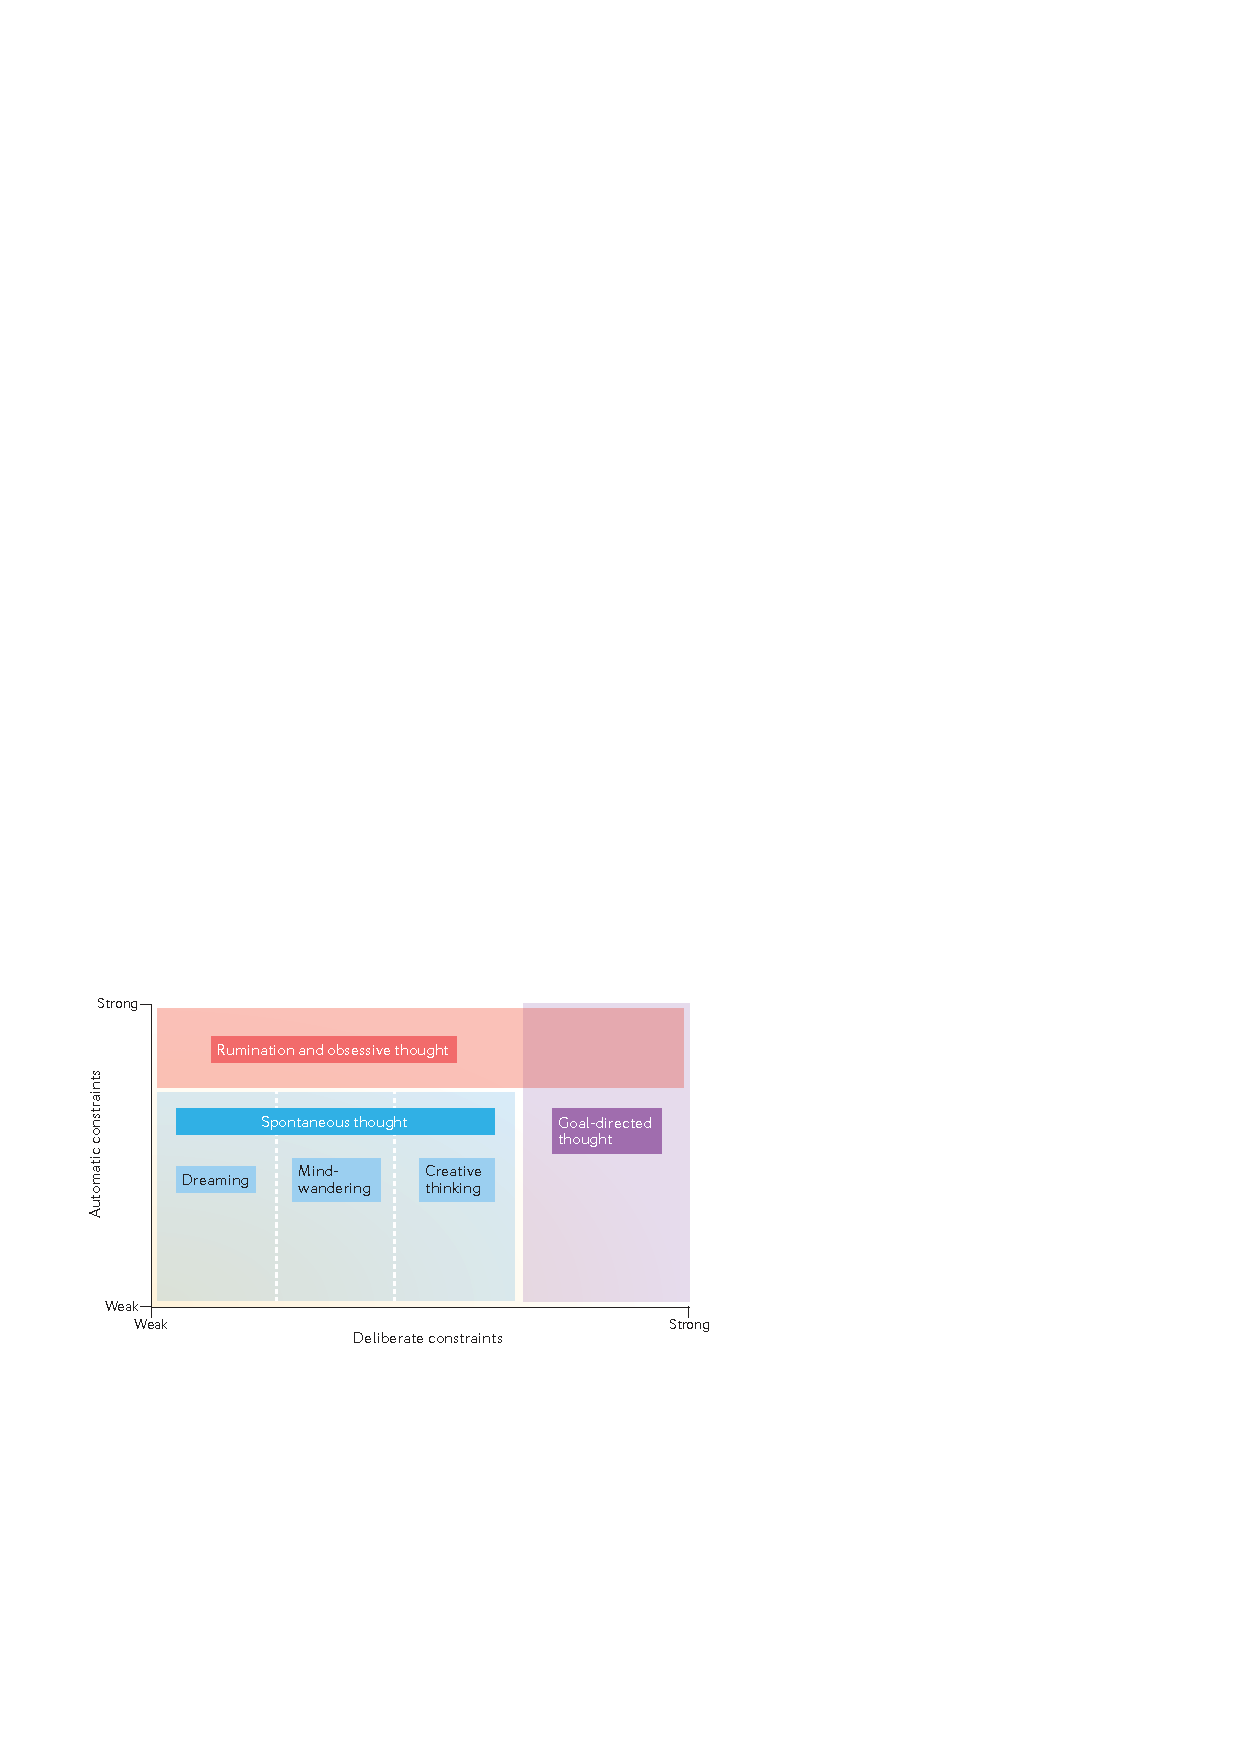
\includegraphics[width=0.75\linewidth]{assets/conceptual_space} 

}

\caption{Conceptual space of different types of thought (Christoff et al., 2016)}\label{fig:conceptual}
\end{figure}

\ldots{}

\subsection{On the verbal and sensory properties of
rumination}\label{on-the-verbal-and-sensory-properties-of-rumination}

\ldots{}

\section{What is that little voice inside my head
?}\label{what-is-that-little-voice-inside-my-head}

\subsection{Brief historical overview of inner speech
investigations}\label{brief-historical-overview-of-inner-speech-investigations}

Description, functions, nature\ldots{}

Soviet psychology\ldots{} marxist psycohlogy\ldots{} Akhutina (2003)
highlihghts a distincion between the study of inner speech (and speech
production in general) in the west based on linguistics and chomsky
work, and its origin in marxist psychology in the east, where language
is to be though in relation to its usages\ldots{}

Vygostky essential properties of inner speech: i) abbreviation, the
phonetic aspect is ``diminished'', reduced, ``In inner speech we do not
need to pronounce a word in its entirety. We understand, by virtue of
our very intention, what word we wanted to say\ldots{} Strictly
speaking, inner speech is almost wordless'' (Vygotsky, 1956, p.~368).
ii) predicativeness, ``Psychologically, inner speech consists of
predicates only''; ``the subject of our inner reason is always present
in our thought''; it is always implicitly understood (Vygotsky, 1956,
pp.~364, 365), iii) it has a semantic structure of its own: predominance
of \emph{sense} over \emph{meaning}\footnote{this refers to Paulhan's
  distinction between the dictionary \emph{meaning} of a word on one
  hand, and the individual \emph{sense} (menaning) of a word, acquired
  by usage, on the other hand.}, it is idiomatic, agglutination of
semantic units, etc.

Therefore, for Vygostky, it follows that the passage from inner speech
to overt speech consists not in simply ``vocalising'' inner speech but
in \emph{restructuring} inner speech (e.g., retrieving a yntax proper to
overt speech, retrieveing the phonetic structure, etc)\ldots{}

In the last chapter of this book, Vygotsky analyzes the relationship
between thought and word in the mature mind. The central idea of this
chapter is stated as follows:

\begin{quote}
The relationship between thought and language is not a thing, but a
process, a continual movement back and forth from thought to word and
from word to thought. Viewed in the light of a psychological analysis,
this relation is a process that passes through a series of phases and
stages, during which its essential features undergo changes that may be
called development in the strict sense. Of course, this is a functional
development, not development in the sense of aging; but the path
traversed by thinking as a process from thought to word is development
nonetheless.
\end{quote}

Vygotsky ends this statement with his famous dictum: \emph{Thought is
not expressed in words; it comes into existence through them} (1956,
p.~330)\ldots{}

\begin{figure}[H]

{\centering 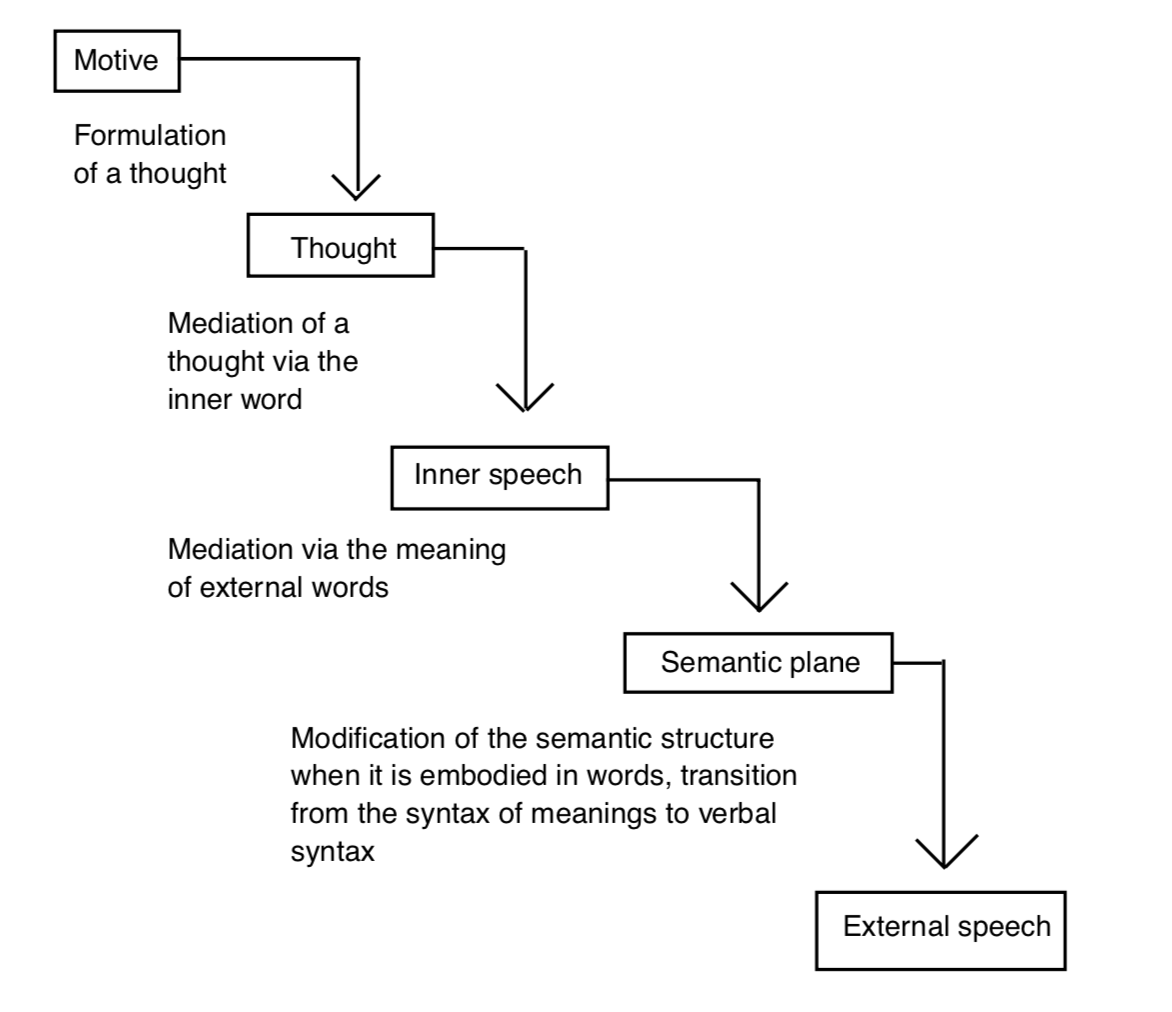
\includegraphics[width=0.75\linewidth]{assets/vygotsky} 

}

\caption{Vygotsky’s Levels in the Process of Verbal Thinking. Figure from Akhtuina (2003).}\label{fig:vygotsky}
\end{figure}

For Luria (1956), a verbal utterance usually starts with a
\emph{motive}\footnote{This includes desires and needs, interests and
  impulses, affects and emotions, etc.}, that is something to express.
For Luria, a veral utterance always starts with a \emph{vague thought}
and the role of inner speech would be to transform this though into
speech. Three stages i) the motive ii) the thought and its
transformation to inner speech and iii) transofrmation to external
speech\ldots{} in his studies of aphasia, Luria (1947) then recognises
thateach of these stages can be (more or less) independently
impaired)\ldots{}

\emph{Copy-pasted from Akhutina (2003): The way was paved for this
hypothesis by Soviet psychology and its notion of the multilevel
structure of inner speech (Anan'ev, 1946, 1960; Sokolov, 1959, 1968). In
Anan'ev's view, one of the indisputable postulates of inner-speech
theory is ``that inner speech is a process that varies in terms of its
readiness to be transformed into external speech.'' For Anan'ev, inner
speech has the following phases\ldots{}}

Watson (\protect\hyperlink{ref-watson_psychology_1919}{1919}) suggested
that thought was rooted in (overt) speech, with maturation leading from
speech to thought.. this hypothesis also applied to reading, with
beginning reader overtly reading and progessively silently
reading\ldots{}

See reed 1916 for an historical perspective\ldots{} this initial
suggestion (by watson) lead to a fruitful line of research about the
muscular bases and/or correlates of thought and inner speech\ldots{}for
instance, Reed (1916) observed that participnts were moving their tongue
and lips (and sometimes whispering) while reading\ldots{}

In a small monograph, Stricker
(\protect\hyperlink{ref-stricker_studien_1880}{1880}) reported
that\ldots{} however, Paulhan (1886) replied that he was able to produce
(innerly) the vowel 1 and maintan the image of other vowels and that he
was able to imagine the sound of any vowel without motor actions or
feelings (images). Maybe this debats illustrates the limitations of the
introspective method\ldots{}which gives birht to experimental methods
atthe beginning of the last century\ldots{} for instance reed (1916)
desrbies an apparatus to examine tongue movements (see Figure XX) and an
experiment to examine the inovlvment of inner spech (and speech motor
processes) in thinking\ldots{}

\begin{figure}[H]

{\centering 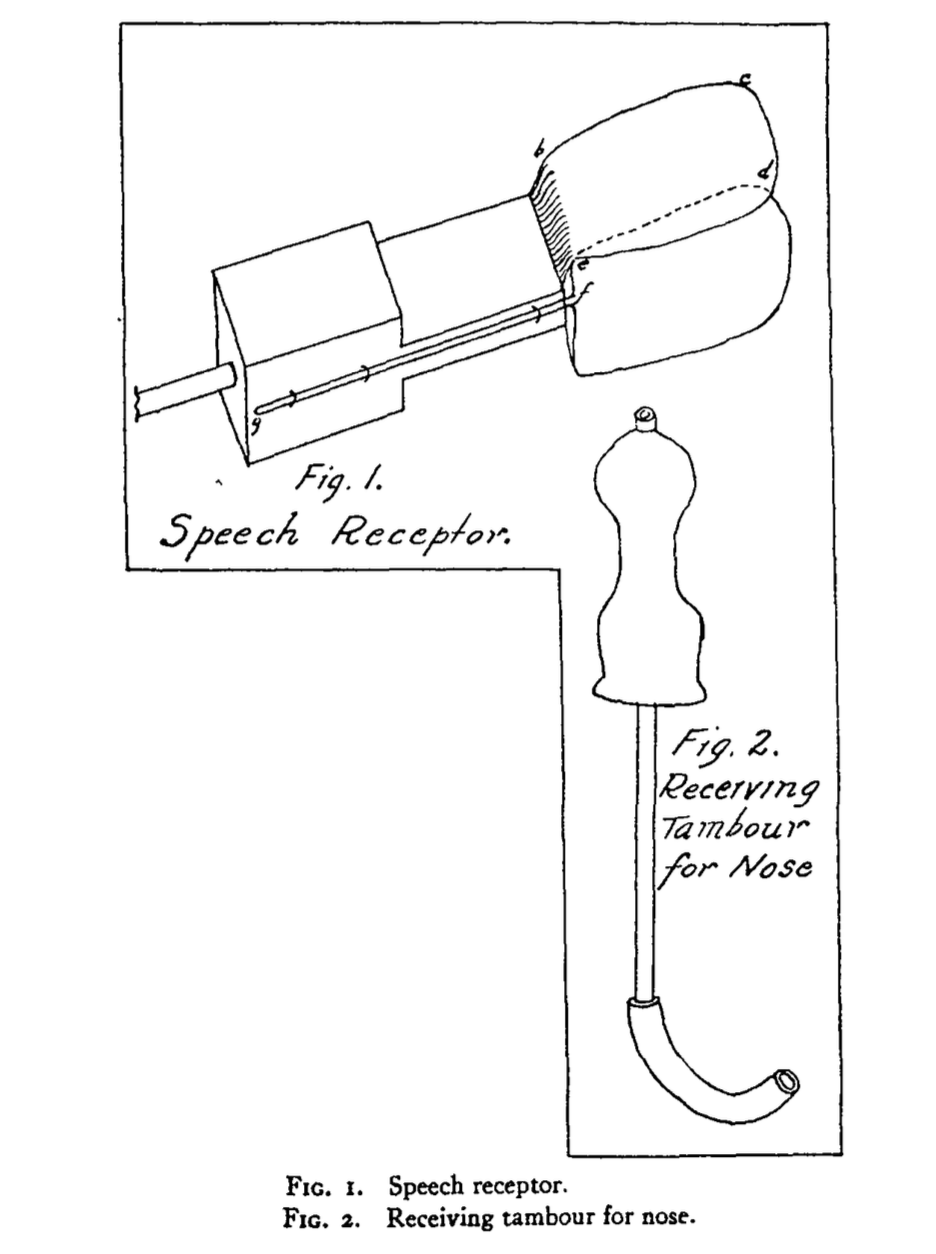
\includegraphics[width=0.5\linewidth]{assets/reed} 

}

\caption{Figure 1 \& 2 from Reed (1916), describing the apparatus used to record tongue movement during thinking and inner speech.}\label{fig:reed}
\end{figure}

Faaborg-Anderson and Edfeldt (1958) found that activity in vocal
musculature increased with difficulty of text (see also Sokolov,
\protect\hyperlink{ref-sokolov_inner_1972}{1972})\ldots{} however it is
not clear that reading always entails inner speech and (or more
precisely), that inner speech always involve
``sub-articulation''\ldots{}discuss counter-examples by the
``anesthesists'' (e.g., Smith, Brown, Toman, \& Goodman,
\protect\hyperlink{ref-smith_lack_1947}{1947})\ldots{}

Historical perspective on the exploration of the role of motor processes
in inner speech, from Sokolov
(\protect\hyperlink{ref-sokolov_inner_1972}{1972}). Dodge (1898)
anesthetised his lips and tongue and ralised that is not impact on his
inner speech. Curtis (1899) and Courten (1902) recorded laryngeal
movements using a pneumatic drum and a kymograph while his participants
recited verses or were reading. They observed that laryngeal movement
were not always present and depended on what was being read and/or
produced, as well as on the ``degree of understanding''\ldots{}

\begin{figure}[H]

{\centering 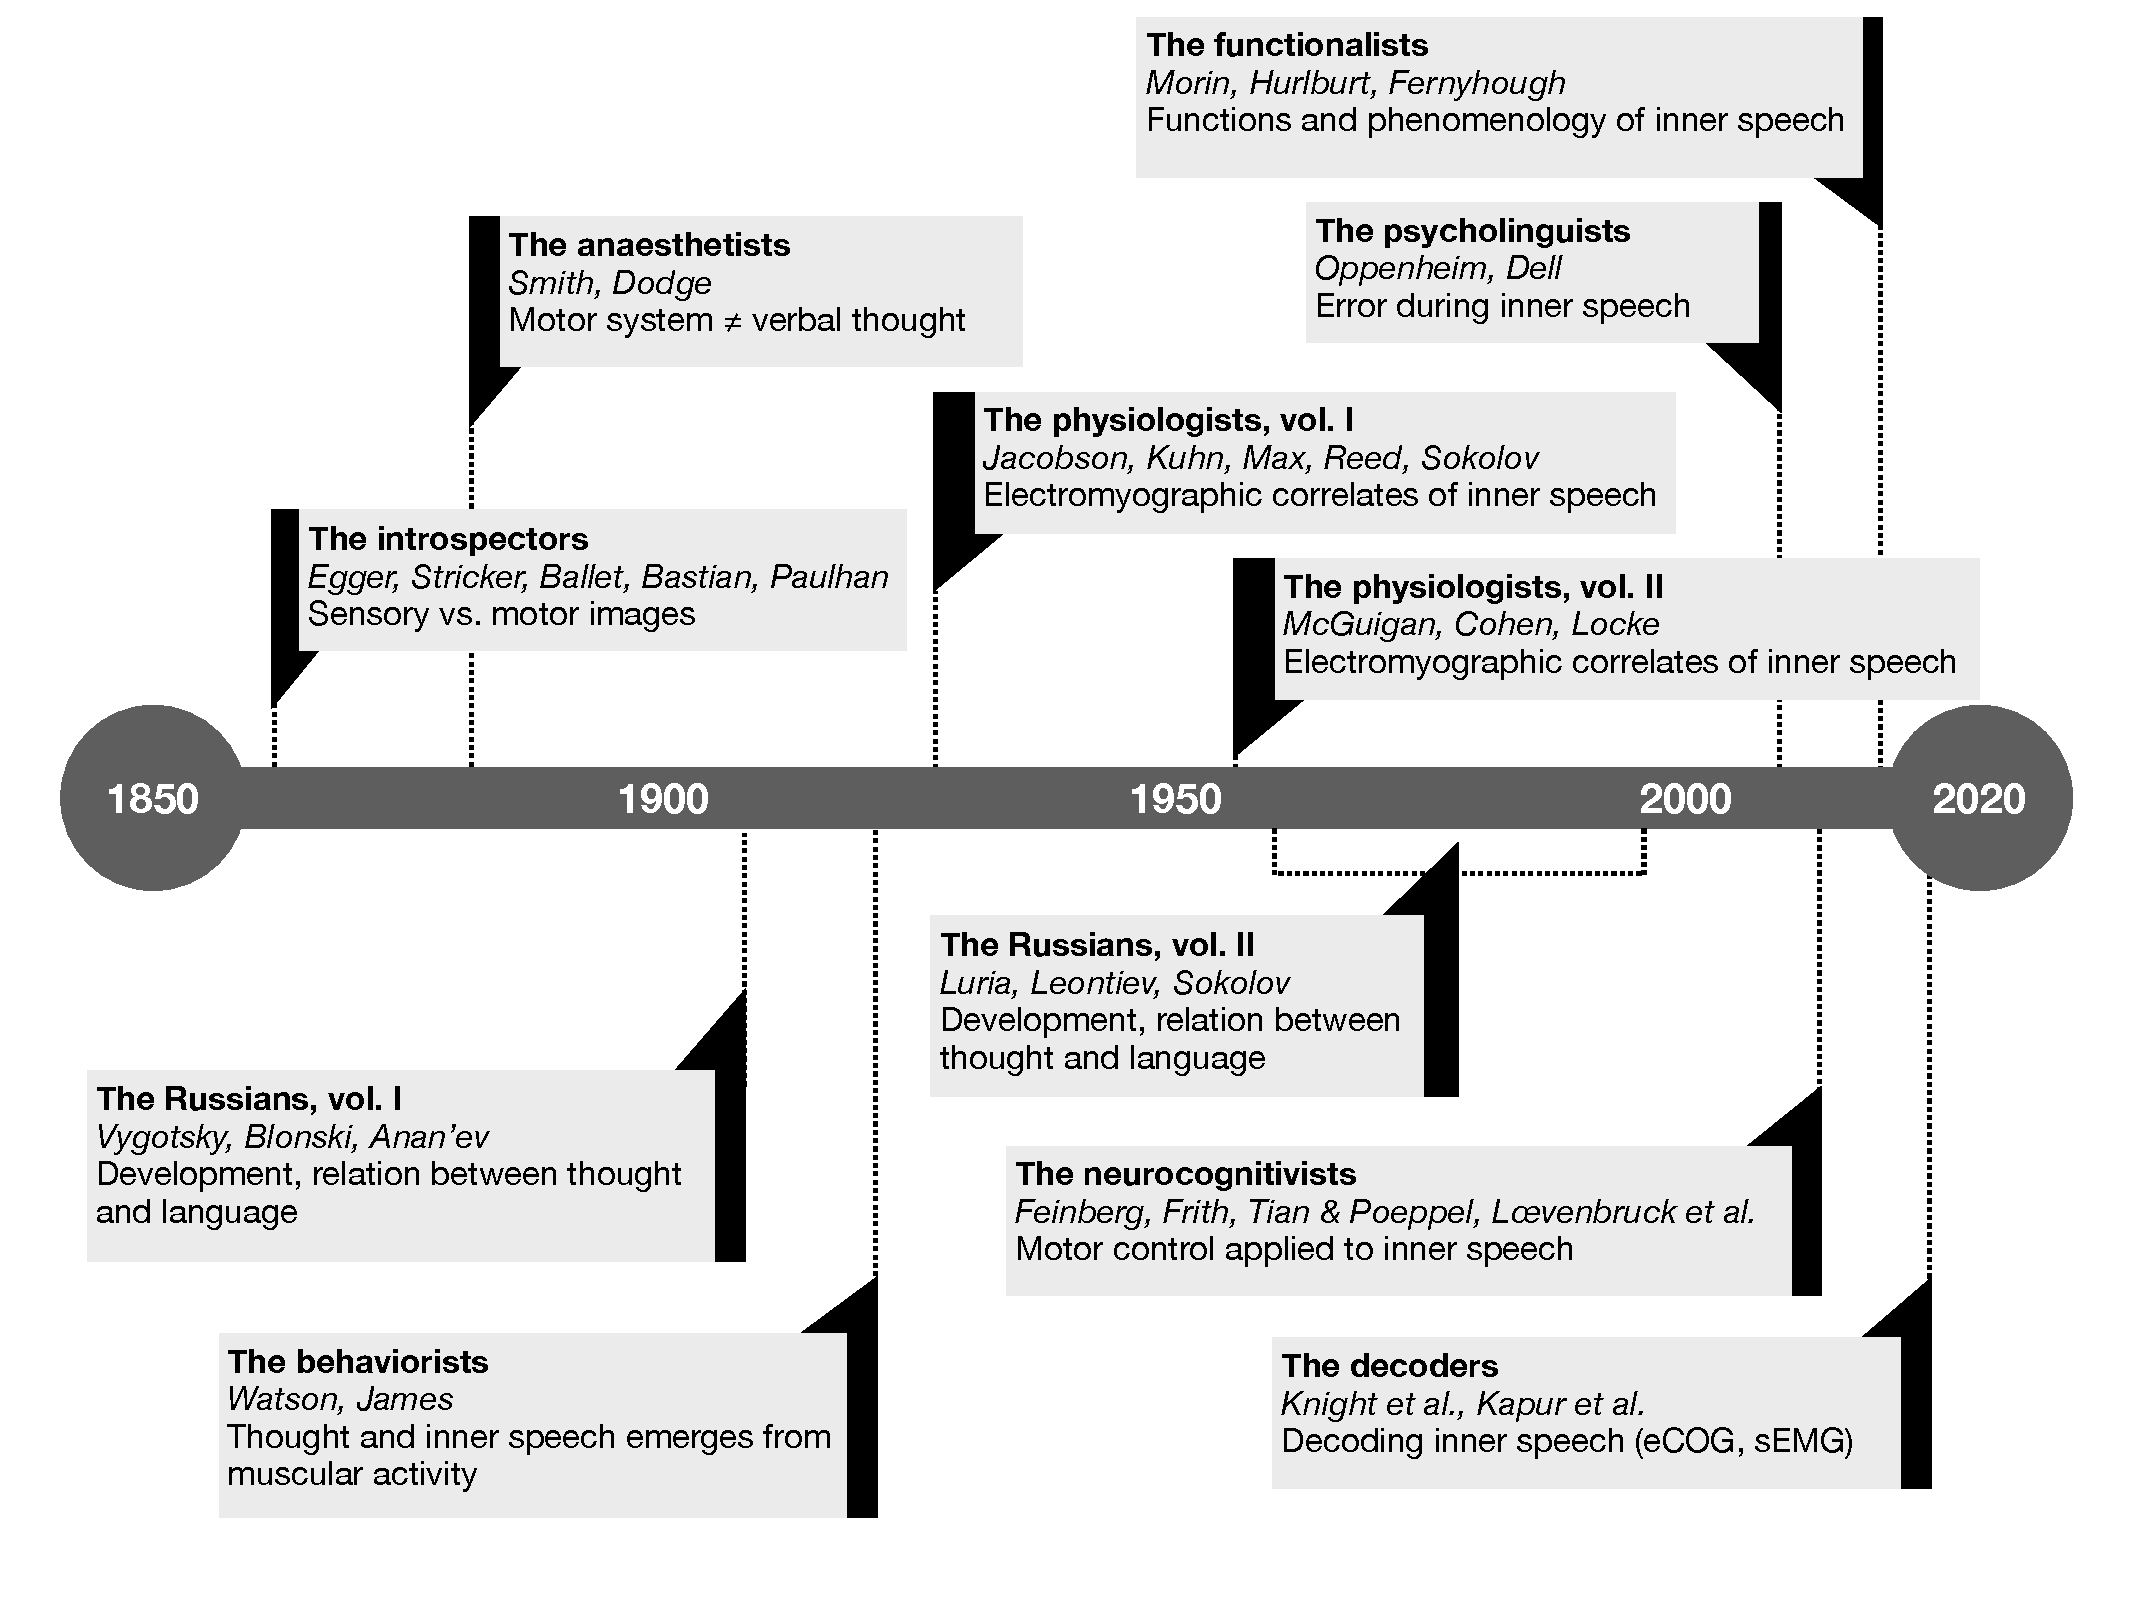
\includegraphics[width=1\linewidth]{assets/timeline} 

}

\caption{Non-exhaustive overview of contemporary inner speech research from 1850 to present days.}\label{fig:timeline}
\end{figure}

Jacobson (\protect\hyperlink{ref-jacobson_electrical_1931}{1931}) used a
galvanometer to record action potentials of tongue and lips muscles and
observed small musles contraction during inner speech production, ``as
if words were pronounced in a rapid and abbreviated manner'' (cited in
Sokolov, \protect\hyperlink{ref-sokolov_inner_1972}{1972}, p. 45).

The discussion of inner speech in soviet Psychology resolved mostly
around the issue of the functions of inner speech. The work of Lev
Vygotsky and PP Blonsky (for instance) culminted in si suggesting that
inner speech is speech ``to oneself'' and ``for oneself''.
Interestingly, Vygotsky rejected both the verbal memory view of inner
speech (i.e., inner speech is simply the retrieval of acoustic, optic or
motor images of words) and the behaviourist view of inner speech as
merely a soundless form ox external speech (à la Watson). For Vygotsy,
the most dtermining factors of inner speech are its semantic
features\ldots{}

Concerning the development of inner speech, Vygostky considered that
inner speech likely dervies from the \emph{egocentric speech}\footnote{According
  to Piaget, the egocentric speech is a conversation of the child aloud
  with herself.} of the preschool child. This lead Vygostky to claim a
functional equivalence between egocentric speech and internal speech,
the later resulting from a progressive internalisation of the
former\ldots{}

Vygostky\ldots{} high \emph{predicativeness} of inner speech (no
subject), because we know what we are talking about\ldots{}
abbreviateness\ldots{}

Sokolov (\protect\hyperlink{ref-sokolov_inner_1972}{1972}) provided
seminal observations that inner speech is involved during reading, to an
extent that is diretly related to the difficulty of the ongoing reading
task. More precisely, he observed that the more difficult the task was,
the stronger the ``speech motor impulses'' (EMG amplitude) in the speech
muscles. Moreover, the difficulty of the task was also related to the
abbreviateness of inner speech. Simpler reading tasks were associated
with abbrevaiated (condensed) inner speech whereas difficult tasks were
associates with ``unfolded'' (expanded) inner speech, and sometimes
externalised (overt) speech\ldots{} Sokolov
(\protect\hyperlink{ref-sokolov_inner_1972}{1972}) also show shown that,
reciprocally, restrictiing the articulators of the participants (e.g.,
by clamping the tongue or lips) impaired the ability of the participants
to complete the task\ldots{}

On the rate of inner speech as compared to overt speech, see R. E.
Anderson (\protect\hyperlink{ref-anderson_speech_1982}{1982}), Mackay
(\protect\hyperlink{ref-mackay_problem_1981}{1981})\ldots{}it would be
15\% to 20\% faster than overt speech (Coltheart,
\protect\hyperlink{ref-coltheart_phonological_1999}{1999})\ldots{}

\subsection{Theoretical perspectives about inner speech
production}\label{theoretical-perspectives-about-inner-speech-production}

The inner voice as the sensory consequence (prediction, see Loevenbruck
et al., 2018) of imagined speech. Analogy with raising the arm: what we
perceive when we imagine raising our arm are the sensory consequences
(e.g., visual) of what would happen if we actually raised our arm, these
are then kind of predictions. The same thing happens during inner speech
production: the inner voice is the predicted auditory consequence of
actual speech, except that it's predicted. The two actions might seem
very different, partly because of differences in the degree of
automaticity. Imagining raising our arm might need a
voluntary/deliberate/conscious (choose a word) intention (i.e., I want
to raise my arm \textgreater{} I raise my arm) while speech imagery
(i.e., inner speech) seems more automatic: we do not expression
consciously the intention to speak, we just speak\ldots{}

Argument about phonological activation during reading, see Abramson \&
Goldinger (\protect\hyperlink{ref-abramson_what_1997}{1997}), cited in
Ehrich (\protect\hyperlink{ref-ehrich_vygotskian_2006}{2006})\ldots{}
inner speech seems most prominent in beginning readers, or when
processing difficult texts (Coltheart, Besner, Jonasson, \& Davelaar,
1979)\ldots{}

Abramson \& Goldinger (\protect\hyperlink{ref-abramson_what_1997}{1997})
investigated the vowel-length effect (i.e., the fact that the length of
the produced vowel depend on the surrounding consonants) was present in
inner speech\ldots{}they shown (in a lexical decisin task) that the
response time was slowr to long-vowel stimuli than to short-vowel
stimuli\ldots{}but they do note, interestingly, that heir data do not
indicate that inner speech is ``\emph{necessayr} for reading; it may
simply be epiphenomenal'' (Abramson \& Goldinger,
\protect\hyperlink{ref-abramson_what_1997}{1997}, p. 1066)\ldots{}

Huey (\protect\hyperlink{ref-huey_psychology_1968}{1968}) proposed that
phonological representations during reading were auditory\ldots{}he
propsoed that reading involves some form of auditory imagery, the voice
in the head (or \emph{inner hearing})\ldots{}he explained that this
voice becams more and more abbreviated (and therefore less auditorily
sailliant) as reader become more skilled (as explaned in Abramson \&
Goldinger, \protect\hyperlink{ref-abramson_what_1997}{1997})\ldots{}in
the same vein, Stricker
(\protect\hyperlink{ref-stricker_studien_1880}{1880}) prposed that
(silent) reading was impossible without movements of larynx and
lips\ldots{}

\subsubsection{The working memory
perspective}\label{the-working-memory-perspective}

\ldots{}A. Baddeley
(\protect\hyperlink{ref-baddeley_working_1986}{1986}) introduces in his
model the osbvocal rehearasal component, whose role is to prevent decay
in short term memory. This tripartite model comprise one central
exectuvie system and two slave systems. Within these slaves systes,
verbal information is rehearsed within the phonological store throuhg a
meachnism know as the phonological loop, acting to prevent memory loss
in short term memory or working memory\ldots{}

\ldots{}whereas studies have shown that children can store verbal
information, the active (silent) rehearsal of verbal information seems
somehow ``deficient'' before the age of 7 years (e.g., Flavell, Beach,
\& Chinsky,
\protect\hyperlink{ref-flavell_spontaneous_1966}{1966})\ldots{} which is
coherent with the Vygostkian predictions discussed earlier\ldots{}

\subsubsection{MVTV Cohen (1986)}\label{mvtv-cohen-1986}

\ldots{}

\subsubsection{Predictive models}\label{predictive-models}

\ldots{}

Speech production involves the fine-grained coordination of more than
100 muscles in the upper part of the body (Simonyan \& Horwitz,
\protect\hyperlink{ref-simonyan_laryngeal_2011}{2011}). In adult humans,
its covert counterpart (i.e., \emph{inner speech} or \emph{verbal
imagery}) has developed to allow the full reconstruction of usual overt
speech situations. In the same way as visual imagery allows to mentally
examine visual scenes, \emph{verbal imagery} can be used as an internal
tool, allowing --amongst other things-- to rehearse or to prepare past
and future speech situations (for a review, see Perrone-Bertolotti,
Rapin, Lachaux, Baciu, \& Lœvenbruck,
\protect\hyperlink{ref-Perrone-Bertolotti2014}{2014}). In consideration
of its self-evident motoric nature, a parallel can be drawn between
verbal imagery and other forms of motor imagery (e.g., imagined walking
or imagined writing). As such, inner speech studies might benefit from
insights gained from the study of motor imagery and the field of motor
cognition (e.g., Haggard,
\protect\hyperlink{ref-haggard_conscious_2005}{2005}; Marc Jeannerod,
\protect\hyperlink{ref-jeannerod_motor_2006}{2006}).

The process of speech internalisation might be similar the
inernalisation of any kind of motor action. Considering inner speech as
any other form of morot action brings some interesting insights. If
speech production can be broadly described as the coordinated motion of
(groups of) muscles that result in some predictable sensory consequences
(e.g.,, auditory, visual, kinesthesic or somesthesic feelings), then it
can be compared to other forms of action. In that sense, the process of
speech internalisation, as the process of ``internalised walking'',
might follow the same general steps. This process can be broadly defined
as the learning of the mapping between some muscular command or patterns
of muscular commands and the associated sensory consequences. Learning
these associations result in the elaboration of an internal model of the
mapping, that permit to predict ongoing actions, but also to simulate
these actions in the absence of any overt movement. In that sense, the
process of inner speech might be considered under the broad category of
imagined actions\ldots{}

Let's consider the analogy between speaking and playing an instrument
(e.g., the piano). Learning how to play piano can be reduced to the
learning and coordination of complex and fine motor sequences, that in
turn produce sensory (kinestheatic, auditory, visual, etc) feedback to
the producer of the action (the agent). It seems that (from a certain
level of analysis), the act of speech can be paralleled with the act of
playing an instrument in that it consists in the coordination of
infinitely complex movements that result in some modifications in the
environment, that in turn generate sensory feedbacks for the agent.
Thus, pursuing the analogy, we could argue that imagining playing an
instrument and imagining speaking (i.e., producing inner speech) might
rest on similar mechanisms (e.g., see O'Shea \& Moran, 2018).

This view is somehow consistent with the Vygotskian view of inner speech
as internalised egocentric (or private) speech but it proposes a formal
mechanism to explain it\ldots{}

\subsubsection{Loevenbruck et al.,
HMOSAIC}\label{loevenbruck-et-al.-hmosaic}

\ldots{}

\begin{figure}[H]

{\centering 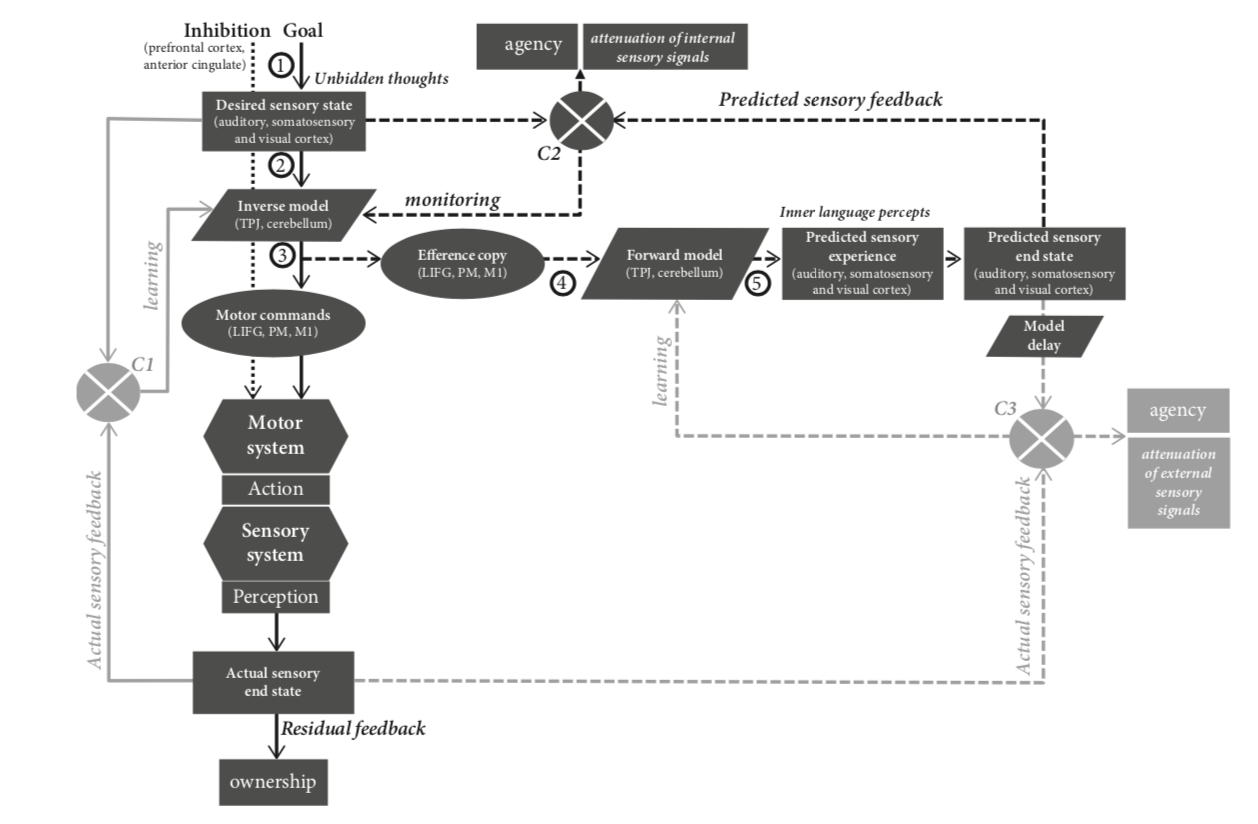
\includegraphics[width=0.75\linewidth]{assets/wolpert} 

}

\caption{...}\label{fig:loevenbruck}
\end{figure}

\subsubsection{Action representation and internal
models}\label{action-representation-and-internal-models}

Voir Marc Jeannerod
(\protect\hyperlink{ref-jeannerod_representing_1994}{1994}) and Wolpert,
Ghahramani, \& Jordan
(\protect\hyperlink{ref-wolpert_internal_1995}{1995}), Wolpert \&
Gharamani (2000)\ldots{}

\vspace{2mm}

\begin{mybox}[label = model]{What is an internal model ?}

Blah blah...

\end{mybox}

\ldots{}

\section{Theoretical perspective on motor
imagery}\label{theoretical-perspective-on-motor-imagery}

Considerable experimental evidence has accumulated to suggest that
movement execution and motor imagery share substantial overlap of active
brain regions (for review, see Guillot, Di Rienzo, MacIntyre, Moran, \&
Collet, \protect\hyperlink{ref-guillot_imagining_2012}{2012}). Such
apparent functional equivalence supports the hypothesis that motor
imageru draws on the similar neural networks that are used in actual
perception and motor control (Gr�zes \& Decety,
\protect\hyperlink{ref-grzes_functional_2001}{2001}; Marc Jeannerod,
\protect\hyperlink{ref-jeannerod_representing_1994}{1994})\ldots{}

See introduction of O'Shea (2017) PhD thesis introduction\ldots{} See
Stinear's chapter in Guillot's book for intracortical and spinal
mechanisms involved during motor imagery (p.55-57).

\subsection{Overt and imagined
actions}\label{overt-and-imagined-actions}

Wittgenstein's (1953) famous query: ``When I raise my arm, what is left
after subtracting the fact that my arm raised?''. We posit that what is
left is an internal model (a representation) of what should happen if
and when my arm goes up (Marc Jeannerod,
\protect\hyperlink{ref-jeannerod_25th_1999}{1999})\ldots{}

\subsection{The motor simulation
theory}\label{the-motor-simulation-theory}

In his seminal paper, Marc Jeannerod
(\protect\hyperlink{ref-jeannerod_representing_1994}{1994}) introduces
the idea of a close functional equivalence between motor imagery and
motor preparation, as suggested by the similar neural and physiological
correlates observed in both imaging and preparing (and by the effects of
motor imagery on motor learning and training). According to Jeannerod,
actions are driven by an ``internally represented world rather than
directly by the external world'' (page 187). In the next paragraph(s),
Jeannerod seems to equate motor representations with motor images or
what he calls \emph{pragmatic representations} (page 187). For
Jeannerod, motor imagery is a part of a broader phenomenon (the motor
representation) related to intending and preparing movements (page 189).
He also echoes the distinction (coming from sport psychology) between
\emph{internal} (imagining an action from the first perspective, which
would be more kinesthesic) and \emph{external imagery} (imagining an
action from the third perspective, which would be more visual). For him,
motor imagery necessarily belongs to the former type (page 189), whereas
the term of \emph{motor imagery} in sport psychology seems to more
broadly ecnompasse both first-person and third-person motor imagery
{[}e.g.,{]}.

Motor preparation is unconscious while motor imagery is conscious.
However, Jeannerod suggests that the difference between the two might be
a difference of degree, rather than one of kind, as the difference
between the two would only be determined by the time spent on each
(i.e., if one makes motor preparation lasting for longer than it's
usually needed, it can ``become'' motor imagery, page 190). In plain
words, the idea is that motor representations/intentions become known to
the subject when they are not followed by execution (page 190), so there
would be a continuum between motor preparation and motor imagery.

EMG lines of evidence page 191: Eye movements have been recorded during
the recall of visual scenes (e.g., Jeannerod \& Mouret 1962). Jacobson
(1930) first suggested that muscles were selectively activated during
imagined action. Shaw (1940) reported that during imagined weight
lifting, electromyographic (EMG) activity of forearm muscles increased
linearly with the magnitude of the weight, etc.

Neural structures and physiological correlates page 192-193.

Evidence from mental chronometry and temporal equivalence (e.g.,
Landauer, 1962), showing that it takes approximately the same amount of
time to say the alphabet or series of numbers aloud and to think them to
himself.

The famous walking + load experiment of Decety, Jeannerod, \& Prablanc
(\protect\hyperlink{ref-decety_timing_1989}{1989}) reveals that force,
rather than duration, is the encoded variable, and that estimated
duration is merely derived from the level of centrally represented
force. When the subjects carried the load, they centrally programmed a
greater force to overcome any resistance, because subjects did not
actually walk (page 194). For Jeannerod, the programming of force as a
subjective correlate: the sensation of effort, which can become
perceptible to the actor independently of overt movement execution and
can be monitored experimentally (page 194). Page 196: representation of
kinematic regularities (e.g., Fitts' law, Viviani's experiments, etc.).

In the following (section 5, starting page 197), Jeannerod develops the
idea that the goal of an action includes an internal representation of
both the external object toward which it is directed and the final state
of the organism when that object has been reached. Then, he develops on
the idea of a distinction between a pragmatic mode and a semantic mode
(page 198). He also makes a distinction between two functions of
representations: a sensory one (to extract from the external world the
attributes of objects or situations that are relevant to a given action)
and a motor one (to encode some aspects of that action) (page 199).

NB: in this paper (Jeannerod, 1994), there is no explicit mention of a
``simulation'' process\ldots{} Jeannerod only discusses the conscious
access to the content of a representation, and defines it as motor
imagery (cf.~notes above as well as the distinction drawn by Grush,
2004). Interestingly, in the commentaries, Morton suggests that many of
the cases Jeannerod reports are actually instances of simulations,
rather than mere imagination, because these cases contain part of what
would be involved in actual performance (page 215). In his response,
Jeannerod seems to agree with and to endorse this view (e.g., page 231).

In the commentary of this paper Gursh suggests that\ldots{} (Motor
models as steps to higher cognition (Rick Grush)) there should exist an
inverse model, and points that nothing mentioned in the target article
is actually capable of generating mental imagery. For Grush, this
inverse model would act centrally, taking as input the efferent copy
(for instance) and would output a mock version of the afferent signals
the peripheral system would have produced given the same input (i.e., an
emulator, see page 209).

For M. Jeannerod (\protect\hyperlink{ref-jeannerod_mental_1995}{1995}),
motor imagery is necessarily first-perspective. Third perspective
imagery is imagery, but not MOTOR imagery\ldots{} Motor representations
are conceived here as `internal models' of the goal of an action.

In Marc Jeannerod (\protect\hyperlink{ref-jeannerod_neural_2001}{2001}),
``Covert and overt stages thus represent a continuum, such that overtly
executed action implies the existence of a covet stage, whereas a covert
action does not necessarily turns out into an overt action'' (page
S103). Jeannerod introduces the term S-states to designate mental stats
which involve an action content and where brain activity can be shown to
simulate that observed during the same, executed, action. These S-states
correspond to intended action, imagined action, and many others (see
Table 1, page S104).

In Marc Jeannerod (\protect\hyperlink{ref-jeannerod_motor_2006}{2006}),
The Simulation Hypothesis of Motor Cognition (pages 129-164). See
Schematic summary of motor simulation according to Jeannerod (page 133).

``Simulation is used here as the off-line rehearsal of neural networks
involved in specific operations such as perceiving or acting (page 129).
According to our view {[}\ldots{}{]}, the simulation relates not to
complete actions but to unspecific elements that comprise actions. Motor
representations are automatically assembled in response to immediate
task requirements and do not rely on memorized actions (page 134).''

The peripheralist versus centralist interpretation of physiological
inner speech correlates (page 153): Subvocal speech was first
interpreted as a source of peripheral kinesthetic information which,
when projected to central nervous structures, generated auditory images
of the corresponding words. The same interpretation was given to the low
intensity EMG recorded during mental motor imagery of limb actions,
which was thought to be the origin of the feelings experienced by the
subject during mental rehearsal (Jacobson 1930), or to the eye movements
recorded during mental visual imagery (e.g.~Brandt and Stark, 1997).
However, this interpretation of mental processes as consequences of
peripheral feedback is now disproved by recent experiments showing
complete absence of muscular activity in many subjects during motor
imagery. When present, this activity is rather assumed to be a
consequence of incomplete inhibition of motor output during mental
states involving motor simulation. This same interpretation might also
hold for inner speech.

Motor imagery can be defined as the mental process by which one
rehearses a given action, without engaging in the physical movements
involved in this particular action. One of the most influential
theoretical explanation of this broad phenomenon, the \emph{motor
simulation theory} (MST, Marc Jeannerod,
\protect\hyperlink{ref-jeannerod_representing_1994}{1994},
\protect\hyperlink{ref-jeannerod_neural_2001}{2001},
\protect\hyperlink{ref-jeannerod_motor_2006}{2006}), contains the three
following postulates at its core: i) there exists a continuum between
the covert (the mental representation) and the overt execution of an
action, ii) action representations can operate off-line, via a
\emph{simulation} mechanism, and iii) covert actions rely on the same
set of mechanisms as the overt actions they simulate, except that
execution is inhibited (O'Shea \& Moran,
\protect\hyperlink{ref-oshea_does_2017}{2017}).

In this framework, the concept of simulation refers to the ``offline
rehearsal of neural networks'' (Marc Jeannerod,
\protect\hyperlink{ref-jeannerod_motor_2006}{2006}), and motor imagery
is conceptualised as a simulation of the covert stage of the same
executed action (O'Shea \& Moran,
\protect\hyperlink{ref-oshea_does_2017}{2017}). The MST shares some
similarities with the theories of embodied and grounded cognition
(Barsalou, \protect\hyperlink{ref-Barsalou2008}{2008}) in that both
allow to account for the phenomenon of motor imagery by appealing to a
simulation mechanism. However, the concept of simulation in grounded
theories is assumed to be multi-modal (not just motoric) and to operate
in order to achieve a particular abstract knowledge (O'Shea \& Moran,
\protect\hyperlink{ref-oshea_does_2017}{2017}), which is not the concern
of the MST\footnote{We should also make a distinction between
  \emph{embodiment of content}, which concerns the conceptual content of
  language, and \emph{embodiment of form}, which concerns ``the vehicle
  of thought'', that is, proper speech production (Pickering \& Garrod,
  \protect\hyperlink{ref-pickering_integrated_2013}{2013}).}.

The MST is supported by a wealth a findings, going from mental
chronometry studies showing that the time taken to perform an action is
often found to be similar to the time needed to imagine the
corresponding action (though not always, see Glover \& Baran,
\protect\hyperlink{ref-glover_motor-cognitive_2017}{2017}, for a review
of controversial findings and for an alternative conceptualisation of
motor imagery), to neuroimaging and neurostimulation studies showing
that both motor imagery and overt actions tend to recruit similar
frontal, parietal and sub-cortical regions (e.g., Hétu et al.,
\protect\hyperlink{ref-hetu_neural_2013}{2013}; Marc Jeannerod,
\protect\hyperlink{ref-jeannerod_neural_2001}{2001}). The involvement of
the motor system during motor imagery is also supported by repeated
observations of autonomic responses and peripheral muscular activity
during motor imagery (we discuss these observations in section XX).

\vspace{2mm}

\begin{mybox}[label = centralism]{Centralism versus peripheralism}

The motor theory of perception: mental states arise from movement (more precisely, from innervation associated with movements (the perceived image of an object arises from the muscular discharges produced during the movements involved in exploring it). The peripheral variant of the motor theory is the idea according to which the mental image of that object is also produced by covert muscular discharges in the related muscles (cf. work from James, 1890; Jacobson, 1930).\\

But the idea developed in this paper is quite the reverse of the peripheral motor theory and would be more akin to a centralist version of the motor theory (page 190). Jeannerod says that existence of muscle discharge during a mental state does not imply a bottom-up influence of these discharges on the mental state. The key phenomenon in Jeannerod’s conception is the motor intention, which is though to be largely endogenous (page 190). Motor imagery would represent the results of conscious access to the content of the intention, and the content of the intention would constrain the expression of the image (page 190). Jeannerod also states that this view is in agreement with the corollary discharge model. The key idea is that the activation of peripheral mechanisms is not needed to generate the image (but they can be activated, as a consequence of the activation of the image/representation)...

\end{mybox}

\subsection{Emulation and internal
models}\label{emulation-and-internal-models}

NB: in this paper emulator is used as a synonym for ``forward models''
(pages 378-379)\ldots{}

Grush (\protect\hyperlink{ref-grush_emulation_2004}{2004}) proposes a
unified framework for explaining a wide variety of representational
functions of the brain: the emulation theory of representation. This
theory has its origins in control theory (forward models) and signal
processing (Kalman filters).

Difference between emulation theory of motor imagery and simulation
theory à la Jeannerod (pages 384-385): ``{[}\ldots{}{]} Given these
definitions, it should be clear that the simulation theory and the
emulation theory are not at all the same thing. They agree that the
efferent motor centers are active during imagery. The simulation theory
takes this by itself to be sufficient for motor imagery; the emulation
theory does not, and claims that in addition, an emulator of the
musculoskeletal system is needed and imagery is produced when the
efferent motor centers drive this emulator. This distinction should be
entirely obvious. To make an analogy: The emulation theory claims that
motor imagery is like a pilot sitting in a flight simulator, and the
pilot's efferent commands (hand and foot movements, etc.) are translated
into faux ``sensory'' information (instrument readings, mock visual
display) by the flight simulator which is essentially an emulator of an
aircraft. The simulation theory claims that just a pilot, moving her
hands and feet around but driving neither a real aircraft nor a flight
simulation, is sufficient for mock sensory information.''

Distinguishing between simulation and emulation theories (page 385):
``{[}\ldots{}{]} The only way to get from the former (signals in motor
format) to the latter (signals in proprioceptive and kinesthetic format)
is to run the motor signal through something that maps motor
plans/signals to proprioception and kinesthesis. And the two
possibilities are (a) the body (yielding real proprioception and
kinesthesis), and (b) a body emulator (yielding faux proprioception and
kinesthesis) {[}\ldots{}{]} A motor plan is one thing, a sequence of
proprioception and kinesthesis is another. The simulation theorist
conflates them.''

In Moulton \& Kosslyn
(\protect\hyperlink{ref-moulton_imagining_2009}{2009}), In brief: they
tried to characterize mental imagery as an information processing
system, considering it in the perspective of Marr's three levels of
explanation (i.e., the computational, algorithmic, and implementation
levels).

Imagery is also characterized by its reliance on perceptual
representations and activation of perceptual brain systems. We use this
conception of imagery to argue that all imagery is simulation--- more
specifically, it is a specific type of simulation in which the mental
processes that `run' the simulation emulate those that would actually
operate in the simulated scenario. This type of simulation, which we
label emulation, has benefits over other types of simulations that
merely mimic the content of the simulated scenario. They note (page
1273): ``{[}\ldots{}{]} `motor imagery' (which actually appears to be
proprioceptive or kinaesthetic imagery---one experiences the bodily
sensations of movement, not the movement commands themselves: Jeannerod,
1994).''

A second class of explanatory models of motor imagery are concerned with
the phenomenon of \emph{emulation} and with \emph{internal models} (see
Gentsch, Weber, Synofzik, Vosgerau, \& Schütz-Bosbach,
\protect\hyperlink{ref-gentsch_towards_2016}{2016}, for a review of the
similarities and dissimilarities of simulation and emulation models).

Internal model theories share the postulate that the motor system is
represented by \emph{internal models}, whose function is to estimate and
anticipate the outcome of a motor command. One of its variant, the
\emph{motor control theory} (e.g., Kawato,
\protect\hyperlink{ref-kawato_internal_1999}{1999}; Wolpert et al.,
\protect\hyperlink{ref-wolpert_internal_1995}{1995}), assumes two kind
of models: a forward model that predicts the sensory consequences of
motor commands from efference copies, and an inverse model that
calculates the feed-forward motor commands from the desired movement
(Gentsch et al., \protect\hyperlink{ref-gentsch_towards_2016}{2016}).

Emulation theories (e.g., Grush,
\protect\hyperlink{ref-grush_emulation_2004}{2004}; Moulton \& Kosslyn,
\protect\hyperlink{ref-moulton_imagining_2009}{2009}) borrow from both
previously discussed framework (i.e., simulation theories and internal
model theories) to posit a specific kind of simulation. While the MST
postulates that during simulation the motor system is guided exclusively
by internal motor representations, the emulation theories suggest that
both motor and sensory systems are emulated in parallel (Grush,
\protect\hyperlink{ref-grush_emulation_2004}{2004}; O'Shea \& Moran,
\protect\hyperlink{ref-oshea_does_2017}{2017}).

In the emulation model proposed by Grush
(\protect\hyperlink{ref-grush_emulation_2004}{2004}), the
\emph{emulator} is a device that implements the same input-output
function as the body (i.e., the musculoskeletal system and relevant
proprioceptive/kinaesthetic systems). When the emulator receives a copy
of the control signal (which is also sent to the body), it produces an
output signal (the emulator feedback), identical or similar to the
feedback signal produced by the body\footnote{In Grush's terminology,
  \emph{emulator} is used as a synonym for \emph{forward models} (see
  Grush, \protect\hyperlink{ref-grush_emulation_2004}{2004}, pp.
  378--379).}. This feedback would be responsible for the presence of
sensory percepts (e.g., visual, auditory, kinaesthetic) during motor
imagery.

One important difference between the emulation theory of motor imagery
and the MST though, is that the latter takes the mere activation of
efferent motor centres as being sufficient for explaining motor imagery,
while the emulation theory postulates that an emulator of the
musculoskeletal system is needed (Grush,
\protect\hyperlink{ref-grush_emulation_2004}{2004}, pp. 384--385). Grush
(\protect\hyperlink{ref-grush_emulation_2004}{2004}) suggested an
analogy to illustrate this difference: ``The emulation theory claims
that motor imagery is like a pilot sitting in a flight simulator, and
the pilot's efferent commands (hand and foot movements, etc.) are
translated into faux ``sensory'' information (instrument readings, mock
visual display) by the flight simulator which is essentially an emulator
of an aircraft. The simulation theory claims that just a pilot, moving
her hands and feet around but driving neither a real aircraft nor a
flight simulation, is sufficient for mock sensory information''.
Alternatively, in the words of Moulton \& Kosslyn
(\protect\hyperlink{ref-moulton_imagining_2009}{2009}), instrumental
simulations (à la Jeannerod) can be thought of as \emph{first-order}
simulations that imitate the content of the simulated action, while
emulative simulations can be thought of as \emph{second-order}
simulations that imitate both the content and the processes that change
the content.

\section{Electromyography of covert
actions}\label{electromyography-of-covert-actions}

\subsection{Explaining the muscular activity during motor
imagery}\label{explaining-the-muscular-activity-during-motor-imagery}

Motor imagery has consistently been defined as the mental rehearsal of a
motor action without any overt movement. One consequence of this claim
is that, in order to prevent execution, the neural commands for muscular
contractions should be blocked at some level of the motor system by
active inhibitory mechanisms (for a review, see Guillot et al.,
\protect\hyperlink{ref-guillot_imagining_2012}{2012}). Despite these
inhibitory mechanisms, there is now abundant evidence for peripheral
muscular activation during motor imagery (for a review, see Guillot \&
Collet, \protect\hyperlink{ref-guillot_contribution_2005}{2005}; Guillot
et al., \protect\hyperlink{ref-guillot_imagining_2012}{2012}). As
suggested by Marc Jeannerod
(\protect\hyperlink{ref-jeannerod_representing_1994}{1994}), the
incomplete inhibition of the motor commands would provide a valid
explanation to account for the peripheral muscular activity observed
during motor imagery. This idea has been corroborated by studies of
changes in the excitability of the motor pathways during motor imagery
tasks. Bonnet, Decety, Jeannerod, \& Requin
(\protect\hyperlink{ref-bonnet_mental_1997}{1997}) measured spinal
reflexes while participants were instructed to either press a pedal with
the foot or to simulate the same action mentally. They observed that
both H-reflexes and T-reflexes increased during motor imagery, and that
these increases correlated with the force of the simulated pressure.
Using transcranial magnetic stimulation and motor evoked potentials
(MEPs), several investigators observed muscle-specific increases of MEPs
during various motor imagery tasks, while no such increase could be
observed in antagonist muscles (e.g., Fadiga et al.,
\protect\hyperlink{ref-fadiga_corticospinal_1999}{1999}; Rossini,
\protect\hyperlink{ref-rossini_corticospinal_1999}{1999})\footnote{As a
  side note, we should remark that these findings are consistent with
  both the simulation and the emulation views on motor imagery.}.

\vspace{2mm}

\begin{mybox}[label = inhibition]{The motor inhibition problem}

The problem of inhibition (page S106): how come that covert actions, in spite of activation of the motor system, do not result in muscular activity and overt movements? Two possibilities:\\

*   Subliminal activation during S-states, insufficient to fire spinal motoneurons

*   Or, activations would be blocked/attenuated before to reach the motoneurons by an inhibitory mechanism generated in parallel to the motor activation...\\

NB: these two possibilities are not necessarily incompatible...

\end{mybox}

Interestingly, the dominant interpretation of the muscular correlates of
motor imagery at the beginning of the last century was that the
peripheral muscular activity observed during imagined actions was the
\emph{source} of the mental content. However, as explained by Marc
Jeannerod (\protect\hyperlink{ref-jeannerod_motor_2006}{2006}), this
interpretation of mental processes as a consequence of peripheral
feedback is now disproved, for instance by the simple fact that many
people can experiment motor imagery, without any observable muscular
activity\footnote{The \emph{peripheralist} interpretation has also been
  disproved by the heroic experiment carried out by Smith et al.
  (\protect\hyperlink{ref-smith_lack_1947}{1947}). Smith used
  d-tubocurarine (curare) to paralyse his own facial muscles in order to
  test this interpretation. He later reported that, while being
  paralysed, he was still able to think in words and to solve
  mathematical problems.}. In the most recent theoretical explanations
of motor imagery (e.g., MST, emulation or internal models theories), the
peripheral activity is rather assumed to be a consequence of an
incomplete inhibition of motor output during the mental states involving
motor simulation/emulation (i.e., these views adhere to a
\emph{centralist} interpretation of the physiological correlates of
inner speech).

\subsection{Controversial findings}\label{controversial-findings}

As reviewed in Guillot, Lebon, \& Collet
(\protect\hyperlink{ref-guillot_electromyographic_2010}{2010}), although
there are many observations showing a peripheral muscular activity
during motor imagery, there are also many studies failing to do so, or
reporting surprisingly high levels of inter-subject variability, with
some participants showing no muscular activity at all. Putting aside the
discussion on the exact nature and location of the inhibitory mechanisms
during motor imagery (see Guillot et al.,
\protect\hyperlink{ref-guillot_imagining_2012}{2012}), two main
explanations have been advanced to resolve these discrepancies. First,
the electromyographic activity recorded during motor imagery could be
moderated by the perspective taken in motor imagery. We usually make a
distinction between a first-person perspective or \emph{internal
imagery} (i.e., imagining an action as we would execute it) and a
third-person perspective or \emph{external imagery} (i.e., imagining an
action as an observer of this action), that seem to involve different
neural and cognitive processes. It has been shown that a first-person
perspective generally results in greater EMG activity than motor imagery
in a third-person perspective (Hale,
\protect\hyperlink{ref-hale_effects_1982}{1982}; Harris \& Robinson,
\protect\hyperlink{ref-harris_effects_1986}{1986}). Second, some authors
postulated that the intensity of the EMG activity recorded during motor
imagery might be related to the individual ability to form an accurate
mental representation of the motor skill (i.e., the vividness of the
mental image). However, after reviewing the available evidence, Guillot
et al. (\protect\hyperlink{ref-guillot_brain_2009}{2009}) concluded that
this is unlikely to be the case. Alternatively, discrepancies in
experimental design and methodological choices (e.g., use of
intramuscular versus surface electromyography) could also explain these
different results (Guillot et al.,
\protect\hyperlink{ref-guillot_electromyographic_2010}{2010}).

In the next section, we turn to a discussion of inner speech
conceptualised as a kind of motor (and sensory) imagery of speech, and
discuss the theoretical underpinnings of this proposition as well as the
available empirical evidence in its support.

\subsection{Electromyographic correlates of inner speech
production}\label{electromyographic-correlates-of-inner-speech-production}

Various terms: internal speech, silent speech, covert speech, implicit
speech, speech imagery\ldots{} difference between generative component
(mackay, 1992) / inner speaking / inner voice and perceptual or auditory
component (MacKay, 1992) or inner hearing / inner ear\ldots{}

A key question: what is the lowest level of specification of inner
speech ? \ldots{} figure from oppenheim \& dell (2010\ldots{})

See MacKay (1992, page 131) for discussion of speaking rate in inner and
overt speech\ldots{} faster rates also occur for other highly trained
skills (e.g., tying a shoelace, Annett, 1988)\ldots{}ref to review of
Guillot\ldots{}

EMG during inner speech (from mckay, 1992): ``interestingly, this same
EMG activity invariably precedes by a few milliseconds the full blown
muscle activity that occurs during normal movements'' (e.g., Schmidt,
1982)\ldots{}

\vspace{2mm}

\begin{mybox}[label = garrity]{Proper control conditions in electromyographic studies of inner speech production}

Guidelines from Garrity (1977) here...

\end{mybox}

While grasping the concept of a visual image appears as relatively
straightforward, it seems more difficult at first to grasp the concept
of a motor image, especially when it comes to verbal imagery. The
subjective experience of the tension that results from a given position
of the articulators and the covert production of an incompatible speech
sound permits to substantiate what a motor image is. For instance, it is
generally impossible to generate the image of the pronunciation of the
sound ``b'' while keeping the mouth wide opened (e.g., Binet,
\protect\hyperlink{ref-binet_psychologie_1886}{1886}; Stricker,
\protect\hyperlink{ref-stricker_studien_1880}{1880}). This simple
experiment allows defining imagined speech as the simulation of the
corresponding overt verbal content, where \emph{simulation} is meant to
be understood either as the off-line rehearsal of neural motor networks
involved in the overt action (Marc Jeannerod,
\protect\hyperlink{ref-jeannerod_motor_2006}{2006}), or in the terms of
the emulation theories discussed previously\footnote{Translated to
  speech, the MST is similar to previous proposals such as the
  \emph{motor theory of voluntary thinking} (Cohen,
  \protect\hyperlink{ref-cohen_motor_1986}{1986}) or the hierarchical
  model of mental practice (Mackay,
  \protect\hyperlink{ref-mackay_problem_1981}{1981}).}.

The model of wilful (voluntary) inner speech production introduced in
Lœvenbruck et al.
(\protect\hyperlink{ref-loevenbruck_cognitive_2018}{2018}) goes one step
further and, by building on the models of speech motor control (e.g.,
Houde \& Nagarajan, \protect\hyperlink{ref-houde_speech_2011}{2011};
Wolpert et al., \protect\hyperlink{ref-wolpert_internal_1995}{1995}),
describes inner speech as ``multi-modal acts with multi-sensory percepts
stemming from coarse multi-sensory goals''. In other words, the auditory
and kinaesthetic sensations perceived during inner speech prediction are
assumed to be the predicted sensory consequences of speech motor acts,
emulated by internal forward models, that use the efference copies
issued from an inverse model (this proposal shares similarities with the
emulation model of motor imagery discussed earlier, Grush,
\protect\hyperlink{ref-grush_emulation_2004}{2004}).

\textbf{Fin de l'intro old de zygoto\ldots{}}

In other words, ``inner speech is nothing but speech to oneself''
(Sokolov, \protect\hyperlink{ref-sokolov_inner_1972}{1972})\ldots{} it
can be considered as a n internalisation, a psychological transofmration
or ``internal projection'' of overt speech (Sokolov,
\protect\hyperlink{ref-sokolov_inner_1972}{1972})\ldots{}

\chapter{Methodological framework}\label{methodological-framework}

\initial{I}n this chapter we briefly introduce some of the key concepts
related to the methods we used in our work. More precisely, we cover the
technical concepts related to speech production mechanisms, to
electromyography and to our statistical approach. Finally, we give an
overview of the following chapters.

\section{Speech production
mechanisms}\label{speech-production-mechanisms}

\subsection{Psychological aspects of speech
production}\label{psychological-aspects-of-speech-production}

How do we (humans) produce speech ? At a biomechanical level, producing
speech means coordinating a complex dynamic system (i.e., the ensemble
of speech muscles and organs) to produce slight perturbations of the air
flow (sound waves). At a psychological level, speech production can be
said to consist in the translation of thoughts into speech, with the
goal of communicating information. Before being communicated however,
the information of interest is submitted to several important
transformations.

Although speech production is an everyday phenomenon, the way this
process is exactly performed is still the subject of lively debates.
However, current models generally agree with the core steps occurring
during speech production. Willem Levelt (Levelt,
\protect\hyperlink{ref-levelt_speaking:_1989}{1989},
\protect\hyperlink{ref-brown_producing_2000}{2000}) proposed an
influential psycholinguistic model of speech production (see Figure
\ref{fig:levelt}). According to this model, speech production can be
described at three levels: \emph{conceptualisation}, \emph{formulation}
and \emph{articulation}. The first step is managed by a component called
the \emph{conceptualizer}, and consists in selecting a conceptual
message to be produced (\emph{message generation}). In other words, the
speaker conceives a comunicative intention that she wishes to reveal to
an interlocutor. This \emph{preverbal message} is then forwarded to
another component, the \emph{formulator}, that handles both
\emph{grammatical encoding} (i.e., selecting the appropriate word or
\emph{lemma}) and \emph{phonological encoding} (i.e., selecting the
appropriate speech sounds).

\begin{figure}[H]

{\centering 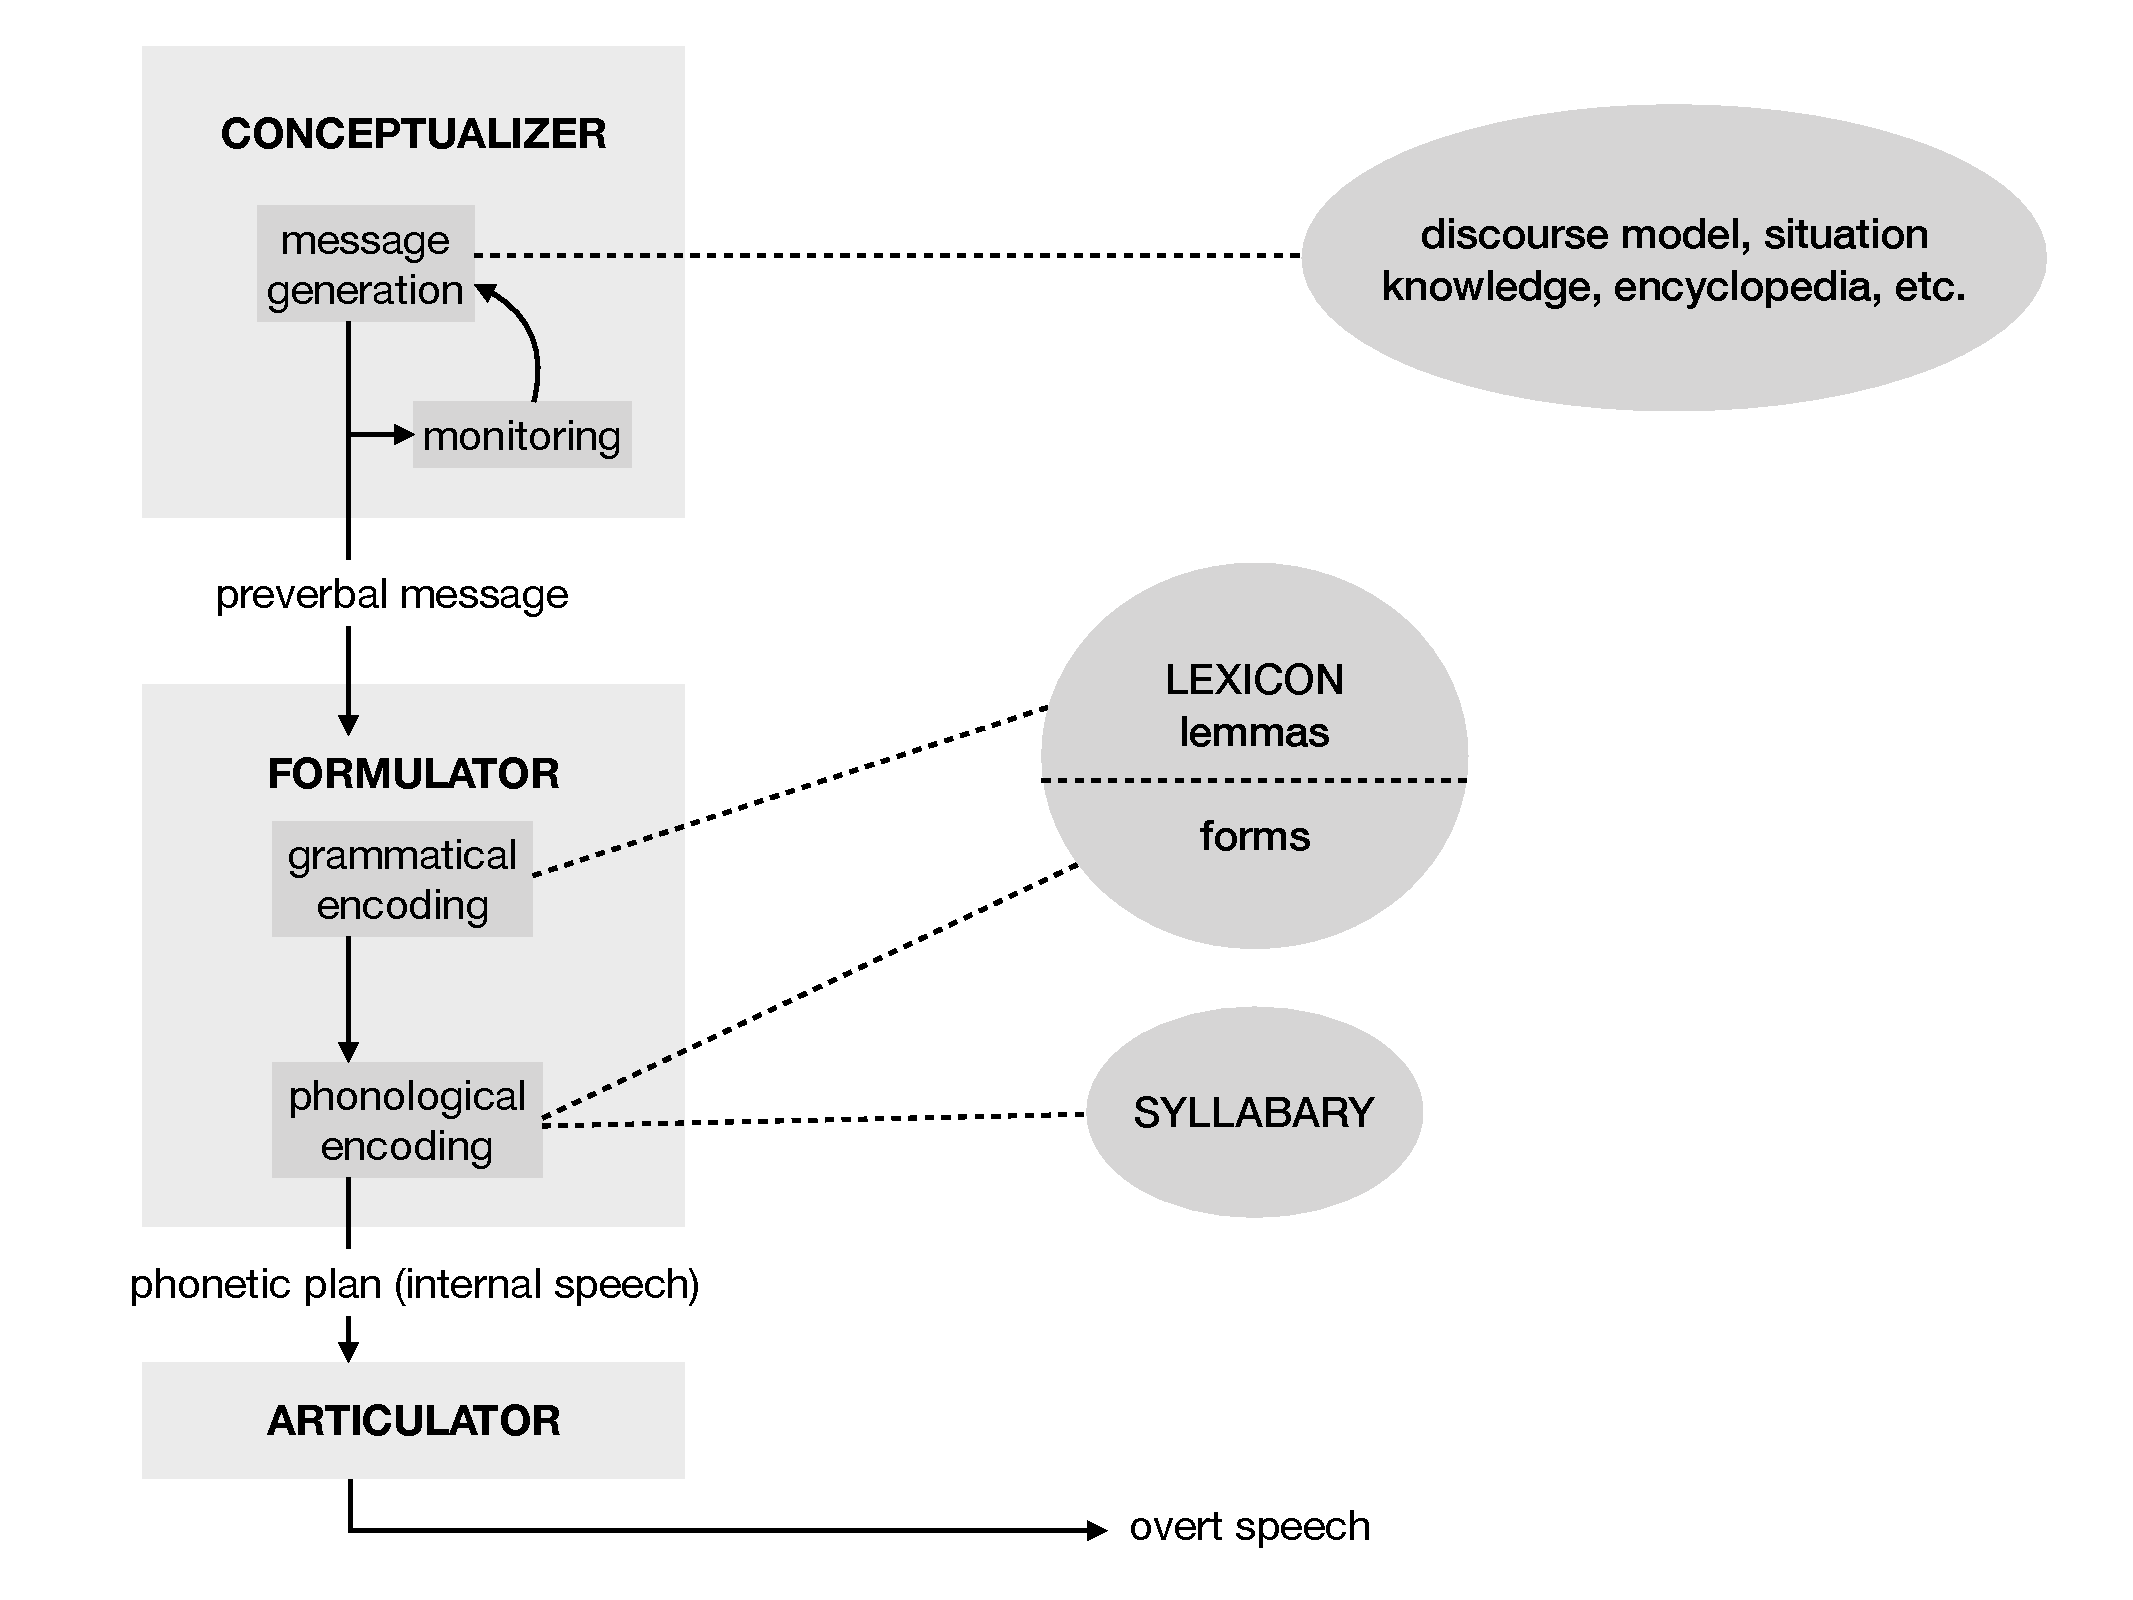
\includegraphics[width=1\linewidth]{assets/levelt} 

}

\caption{Illustration of Levelt's (1989, 2000) model of speech production.}\label{fig:levelt}
\end{figure}

During \emph{grammatical encoding}, \emph{lemmas} are retrieved from the
\emph{lexicon} and are ordered in a syntactical appropriate way, giving
the message its \emph{surface structure}. During \emph{phonological
encoding}, the message is given its phonetic or articulatory
characteristics. At this stage, phonemes are grouped into pronounceable
syllables. Then, each syllable is associated with an \emph{articulatory
program}, composed of an ensemble of \emph{articulatory gestures} (i.e.,
coordinative structures of movements). These articulatory programs are
stored in the \emph{syllabary}. In brief, the \emph{formulator}
component transforms a \emph{preverbal message} into a linguistic
object. Finally, the phonetic plan\footnote{Interestingly, in this model
  the phonetic plan is thought to correspond to inner speech.} is
forwarded to the \emph{articulator}, responsible for the activation of
\emph{articulatory gestures}, to be executed by the speech
\emph{articulators} (e.g., tongue, lips, jaw).

This model permits to explain how a communicative intention is
transformed into speech acts. However, it does not explicitly account
for how speech acts are executed by the articulators. In the next
section, we briefly introduce some of the cores principles related to
the biomechanics of speech production.

\subsection{Biomechanical aspects of speech
production}\label{biomechanical-aspects-of-speech-production}

\subsubsection{Vocal apparatus}\label{vocal-apparatus}

Speech production requires the involvement of more than 100 muscles in
the face, the neck and the chest (Simonyan \& Horwitz,
\protect\hyperlink{ref-simonyan_laryngeal_2011}{2011}). The activity of
these muscles is coordinated to produce an air flow moving from the
lungs to the oral and nasal cavities, via the trachea, the larynx and
the pharynx (see Figure \ref{fig:vocal}). Broadly speaking, speech
production can be said to consist essentially in i) \emph{phonation},
which refers to the manipulation of the air flow and to the vibration of
the vocal folds and ii) \emph{articulation}, which refers to movements
of the \emph{articulators}. The action of the \emph{articulators} (e.g.,
lips, tongue) is to shape the oral and nasal cavities, resulting in
modifications of the sound waves and in the production of different
vowels.

\begin{figure}[H]

{\centering 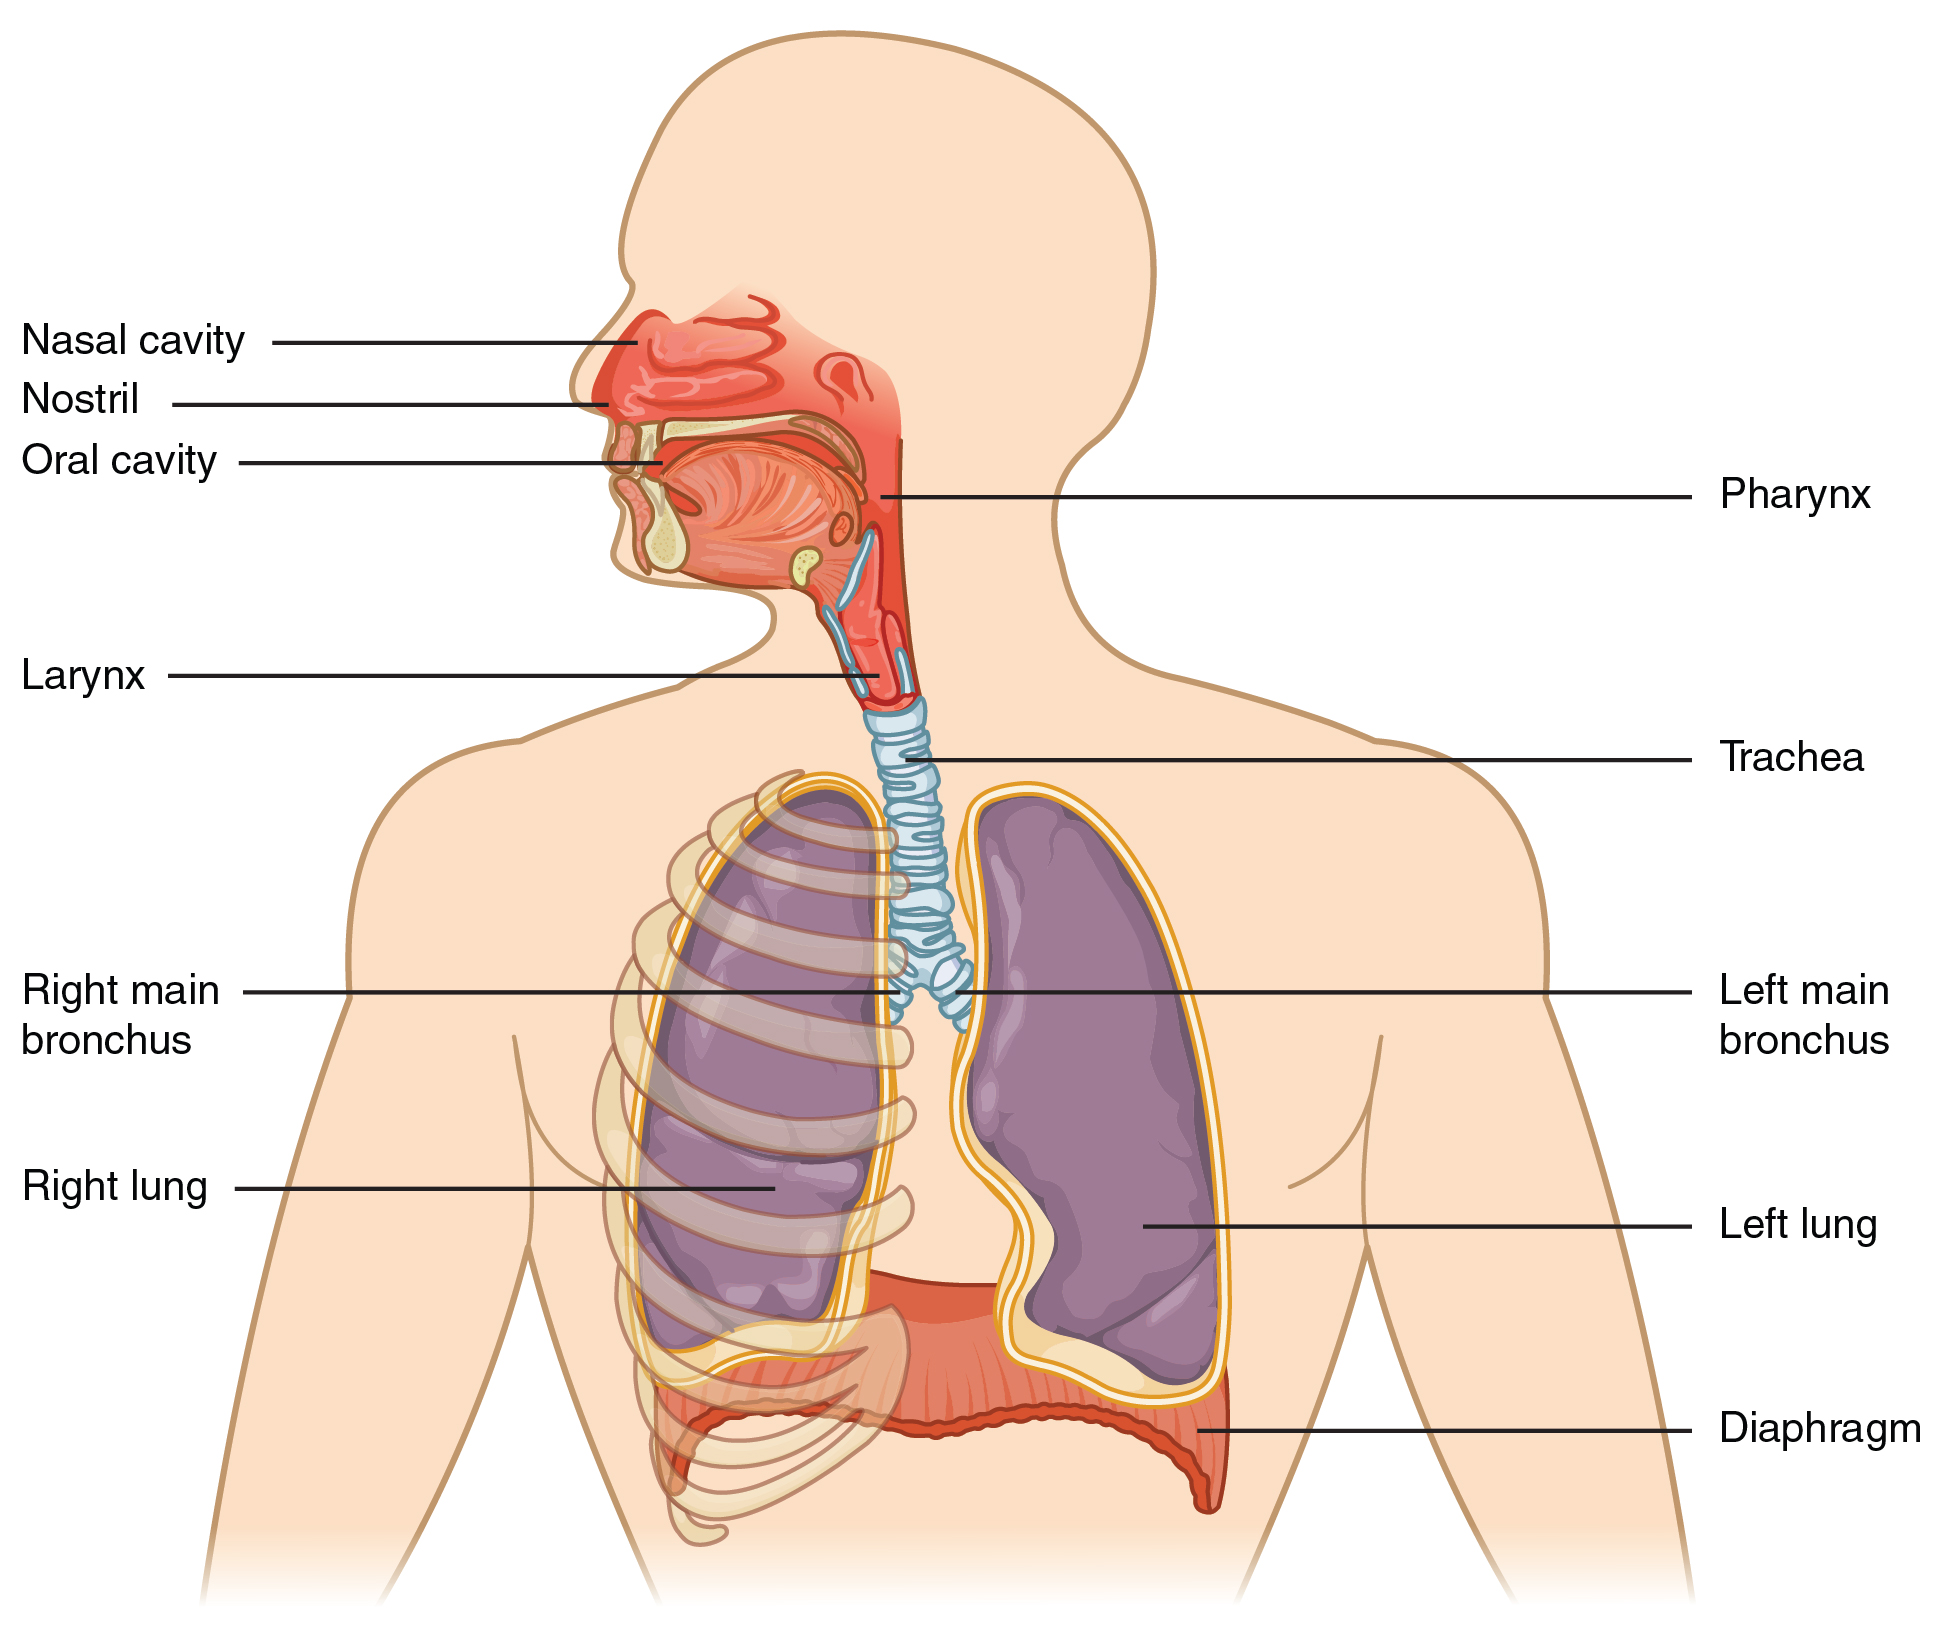
\includegraphics[width=0.75\linewidth]{assets/vocal} 

}

\caption{Human respiratory and phonatory system. Figure from the OpenStax \textit{Anatomy and Physiology} Textbook. Download for free at http://cnx.org/contents/14fb4ad7-39a1-4eee-ab6e-3ef2482e3e22@15.1.}\label{fig:vocal}
\end{figure}

The characteristics of the vocal folds (e.g., their length or thickness)
influence what is known as the \emph{fundamental frequency} (or F0) of
the speech signal, which in turn determines the perceived pitch of the
voice. The speech signal can be further decomposed in \emph{resonant
frequencies} or \emph{formants}. Interestingly, we can relate changes in
the state of the articulatory system with changes in the formant (and
especially the F1-F2) space (see Figure \ref{fig:ipa}). Indeed, the
frequency of the first formant (F1) is mostly determined by the height
of the tongue body whereas the frequency of the second formant (F2) is
mostly determined by the frontness/backness of the tongue body. For
instance, when producing the /u/ vowel, the tongue is positioned at the
top and in the back of the oral cavity (and the lips are rounded).
However, when producing the /a/ vowel, the tongue is positioned at the
bottom of the oral activity (and the lips are widely opened).

\begin{figure}[H]

{\centering 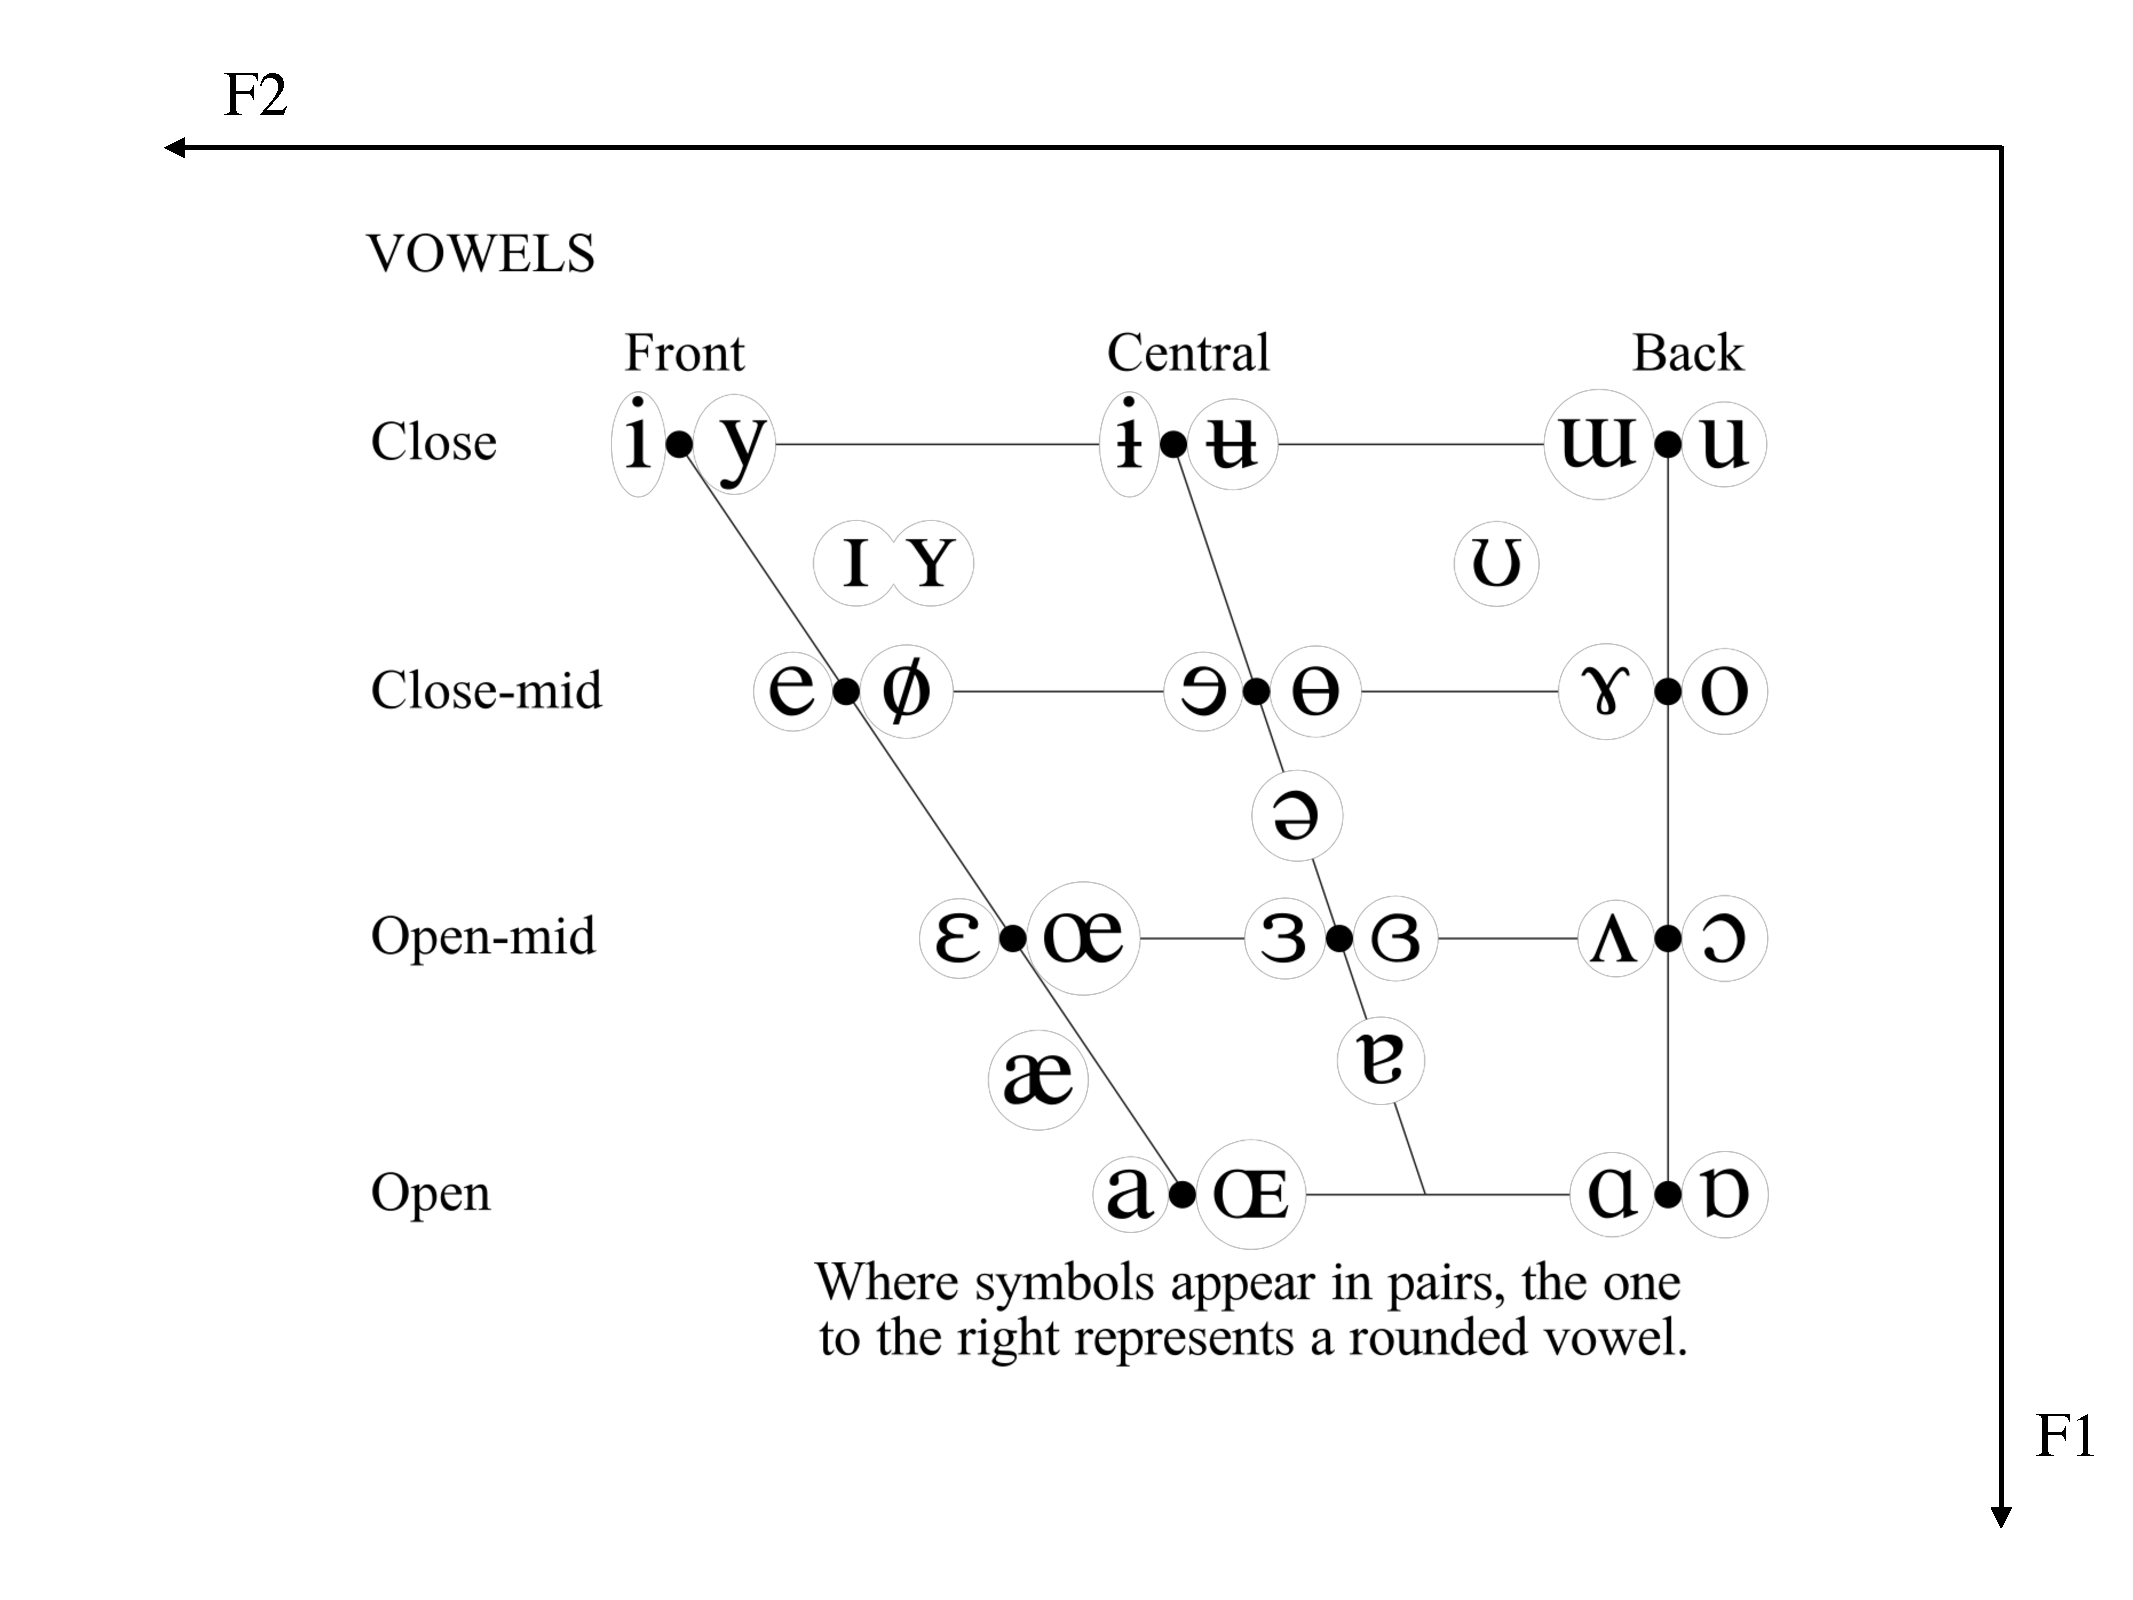
\includegraphics[width=0.75\linewidth]{assets/vowels} 

}

\caption{Illustration of the vocalic 'quadrilateral' and the relation between vowels and formants (F1 and F2). Figure adapted from the International Phonetic Association (2015) - IPA Chart, available under a Creative Commons Attribution-Sharealike 3.0 Unported License.}\label{fig:ipa}
\end{figure}

In brief, modifications in the shape of the \emph{vocal tract} result in
the production of different vowels. Changes in the configurations of
articulators such as the lips or the tongue may also produce consonants.
Consonants are produced by applying some form of restriction to (or by
closing) the vocal tract to constraint the air flow. We usually classify
consonants according to \emph{where} (the \emph{place of articulation})
and \emph{how} (the \emph{manner of articulation}) this restriction
takes place (see Figure \ref{fig:consonants}). For instance, consonants
such as /p/ or /b/ are produced by putting the lips together and are
therefore known as \emph{bilabial} consonants.

\begin{figure}[H]

{\centering 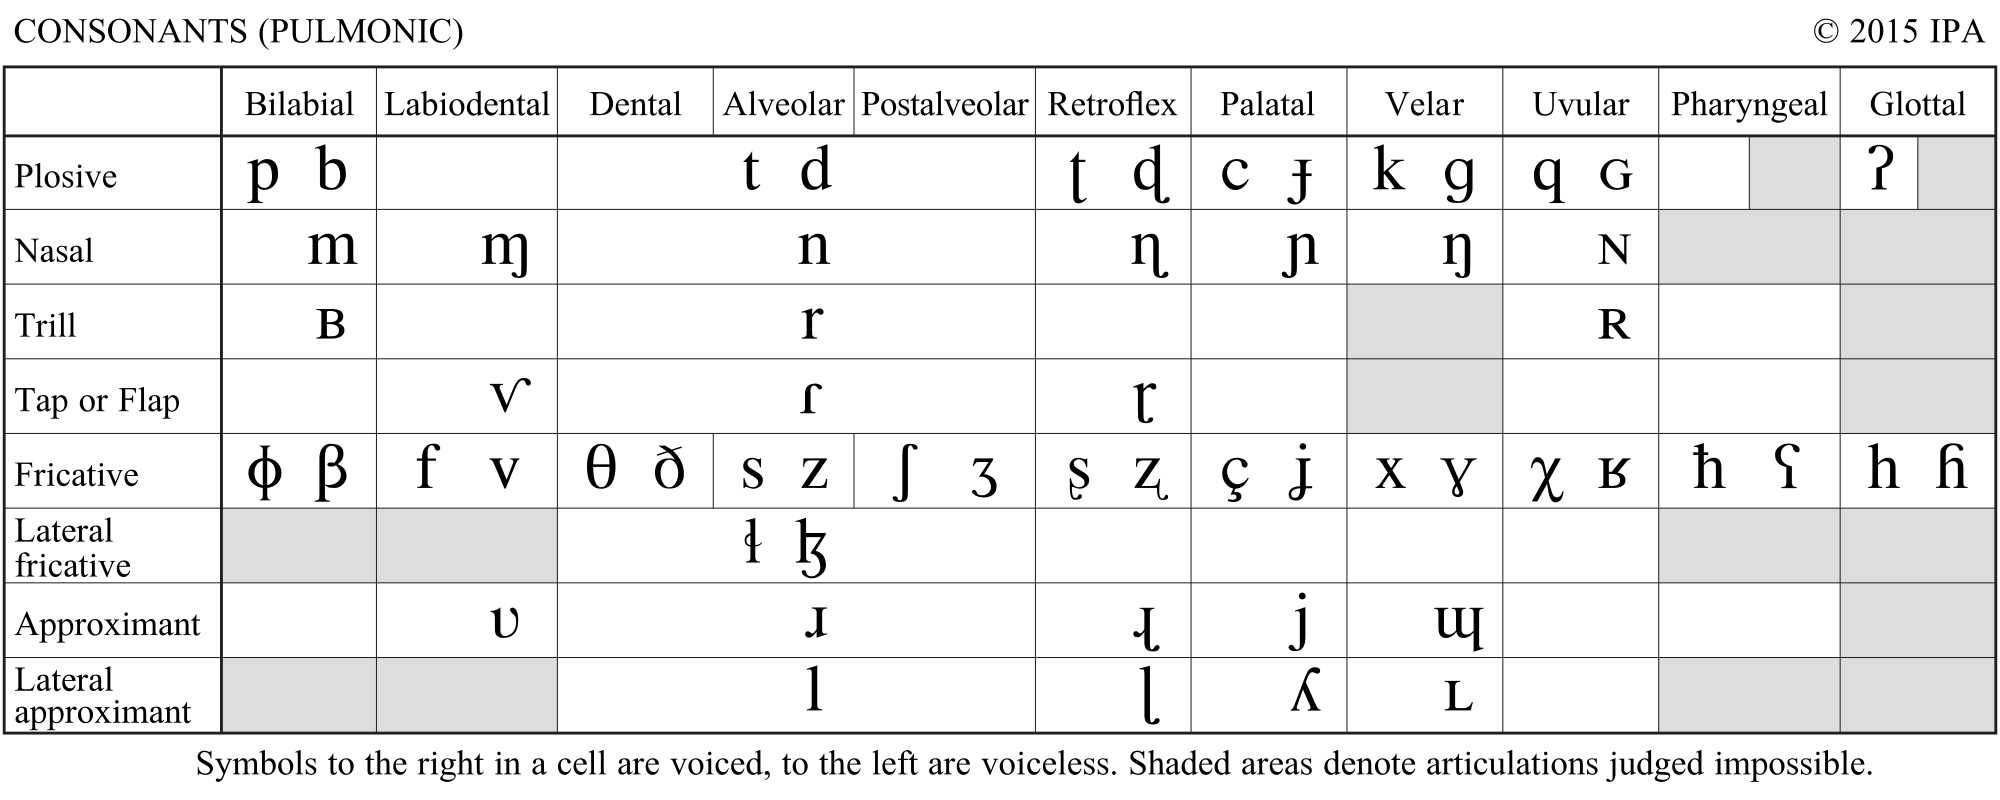
\includegraphics[width=1\linewidth]{assets/consonants} 

}

\caption{Table of consonants according to the manner (in rows) and place (in columns) of articulation. Figure from the International Phonetic Association (2015) - IPA Chart, available under a Creative Commons Attribution-Sharealike 3.0 Unported License.}\label{fig:consonants}
\end{figure}

To sum up, besides from being an essential communication tool for
humans, speech production is also a complex motor action, involving the
fine-grained coordination of numerous muscles. In the next section, we
discuss in more details the specific facial muscles that were of
interest in the present work.

\subsubsection{Orofacial speech muscles}\label{orofacial-speech-muscles}

In our work, we were especially interested in the activity of some of
the orofacial muscles (i.e., the muscles situated around the mouth).
More precisely, we studied the activity of the \emph{orbicularis oris
inferior} (OOI), the \emph{orbicularis oris superior} (OOS), and the
\emph{zygomaticus major} (ZYG) muscles (cf.~Figure \ref{fig:facial}).
Contrary to what was assumed until recently, the \emph{orblicularis
oris} muscle is not a sphincter muscle but is instead a complex of
several distinct muscles that interlace in a way that gives the
\emph{orbicularis oris} complex its circular aspect. Among these
muscles, the OOS and the OOI are placed above and below (respectively)
the mouth and are responsible for rounding or protruding the lips. More
precisely, the OOS is responsible for lowering the upper lip whereas the
OOI is responsible for elevating the lower lip. The ZYG muscle has its
origin on the zygomatic bone and inserts at the labial commissure (the
angle of the mouth) where it meets with fibers of the \emph{levator
anguli oris} and \emph{orbicularis oris} muscles. Together with the
\emph{levator anguli oris}, it serves to move the labial commissure
upwards and laterally, and is involved in laughing and more generally in
pleasant reactions and positive emotions. It is also involved in speech
production, especially during the production of \emph{spread} sounds,
that is, sounds that require a wide aperture of the mouth (e.g., /i/).

\begin{figure}[H]

{\centering 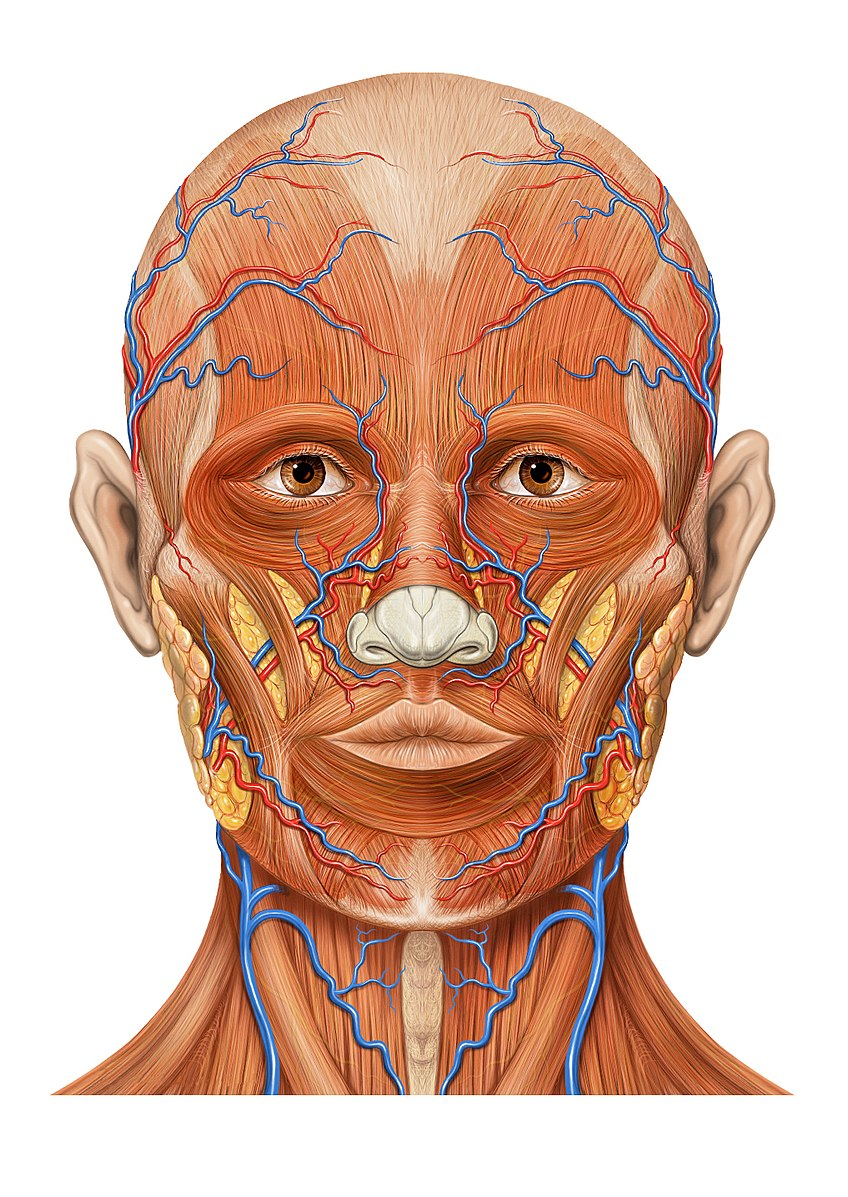
\includegraphics[width=0.75\linewidth]{assets/facial_muscles} 

}

\caption{Illustration of the main facial muscles of interest in the present work. Figure adapted from Patrick J. Lynch, medical illustrator, http://patricklynch.net.}\label{fig:facial}
\end{figure}

For sensors placement, we followed guidelines and recommendations from
Fridlund \& Cacioppo
(\protect\hyperlink{ref-fridlund_guidelines_1986}{1986}). In addition to
speech-related orofacial muscles, we also routinely recorded the
activity of other facial muscles such as the \emph{frontalis} muscle
(FRO) in Chapter 3, 4, 5, and the \emph{corrugator supercilii} muscle
(COR) in Chapter 5. The activity of these muscles was monitored to
control for non speech-related facial muscular activity (as recommended
by Garrity,
\protect\hyperlink{ref-garrity_electromyography:_1977}{1977}).

There are several ways to probe the involvement of specific articulators
in a given speech production task. For instance, it is possible to
selectively interfere with the activity of some articulators (or groups
of articulators) to demonstrate their essential involvement in this
particular task. It is also possible to record the activity of facial
muscles peripherally using surface electromyography, without interfering
with (or with minimal interference to) the natural course of the speech
production process. In the next section, we briefly introduce some core
concepts of electromyography.

\section{A brief introduction to
electromyography}\label{a-brief-introduction-to-electromyography}

Technically speaking, electromyography (EMG) is an experimental
technique concerned with the recording and analysis of myoelectric
signals (i.e., signals resulting from physiological variations in the
state of muscle fibers membranes). Broadly speaking, EMG is a measure of
the electrical activity generated during muscle contraction. It is used
both as a basic tool in (for instance) biomechanical and
psychophysiology research and as an evaluation tool in applied research
(e.g., physiotherapy, rehabilitation, human-computer interfaces). To
facilitate the interpretation of the EMG signal, it is useful to briefly
detail the meaning of its physiological components.

\subsection{Nature of the EMG signal}\label{nature-of-the-emg-signal}

\subsubsection{Muscular anatomy and
physiology}\label{muscular-anatomy-and-physiology}

A muscle is a collection of fibers that can vary in length, orientation,
diameter, and architectural characteristics. For instance, deeper muscle
fibers are usually composed of a greater proportion of slow-twitch
fibers (type I muscle fibers) whereas more superficial muscle fibers
comprise a greater proportion of larger and fast-twitch fibers (type II
muscles fibers, Kamen \& Gabriel,
\protect\hyperlink{ref-kamen_essentials_2010}{2010}). On the basis of
their structure and contractile properties, we can identify three types
of muscle tissues: i) the \emph{skeletal muscles} are attached to bones,
their function is to produce voluntary movements and to protect the
organs, ii) the \emph{cardiac muscles}, whose function is to pump blood
and iii) the \emph{smooth muscles}, involved in involuntary movements
(e.g., respiration, moving food).

The contraction of the skeletal muscles is initiated by electrical
impulses that propagate from the central nervous system to the muscle
via the \(\alpha\)-motoneurons. Interestingly, many (both larger and
smaller) muscles are partitioned, with each portion having a specific
role for the muscle function. Moreover, there is no one-to-one mapping
between populations of motor neurons and muscle compartments. In other
words, one population of motoneurons may innervate several compartments
and reciprocally, several populations of motoneurons may innervate the
same muscle compartment. Therefore, interpreting the EMG signal requires
to be aware whether the recorded signal is characteristic of a whole
muscle' activity or of a specific muscle compartment (Kamen \& Gabriel,
\protect\hyperlink{ref-kamen_essentials_2010}{2010}).

\begin{figure}[H]

{\centering 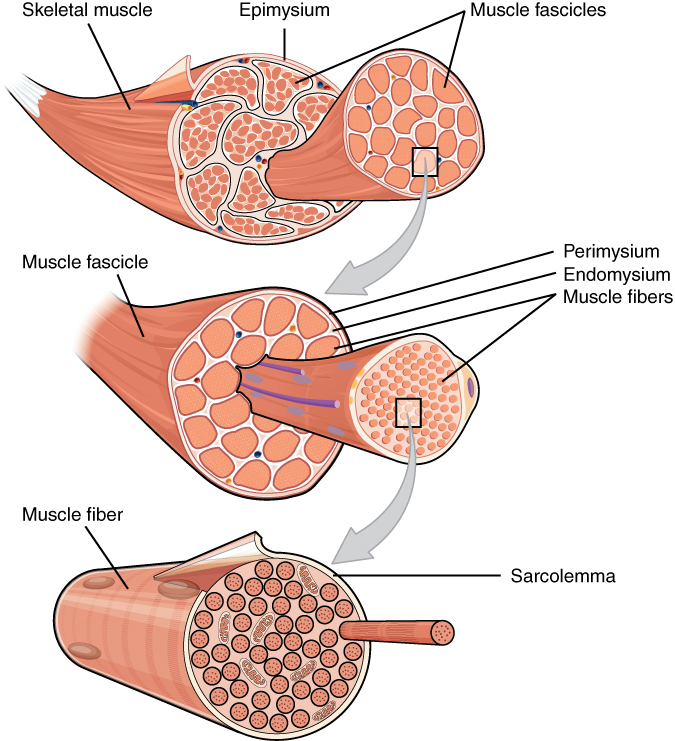
\includegraphics[width=0.5\linewidth]{assets/muscle} 

}

\caption{Illustration of a muscle fiber. Figure from the OpenStax \textit{Anatomy and Physiology} Textbook. Download for free at http://cnx.org/contents/14fb4ad7-39a1-4eee-ab6e-3ef2482e3e22@15.1.}\label{fig:muscle}
\end{figure}

The muscle fiber is surrounded by a membrane, the \emph{sarcolemma} (see
Figure \ref{fig:muscle}). Under resting conditions, the voltage inside
the membrane is around -90mV, relative to the outside. This voltage
results from a particular combination of sodium (\(\text{Na}^{+}\)),
potassium (\(\text{K}^{+}\)), chloride (\(\text{Cl}^{-}\)), and other
anions. At rest, the concentration of \(\text{Na}^{+}\) is relatively
high outside the membrane and relatively low inside the membrane. The
concentration of \(\text{K}^{+}\) follows an opposite pattern, with a
greater concentration inside the membrane, and a lower concentration
outside the membrane.

\subsubsection{The motor action
potential}\label{the-motor-action-potential}

Because muscle membranes can change their electrical state, muscle
fibers are excitable tissues. When a muscle fiber is depolarised, the
\emph{membrane potential} produces a response called the \emph{muscle
fiber ation potential} or more generally the \emph{motor action
potential} (MAP). The generated action potential proceeds along the
muscle fiber in both directions from the neuromuscular junction (Kamen
\& Gabriel,
\protect\hyperlink{ref-kamen_essentials_2010}{2010})\footnote{The
  \emph{neuromuscular junction} is the site where the motoneuron meets
  the muscle fiber.}. In the first phase of the MAP, the
\(\text{Na}^{+}\) permeability increases dramatically, inducing a
massive income of \(\text{Na}^{+}\) into the cell. This results in a
temporary inversion of the cell polarity (see Figure \ref{fig:mfap}).

\begin{figure}[H]

{\centering 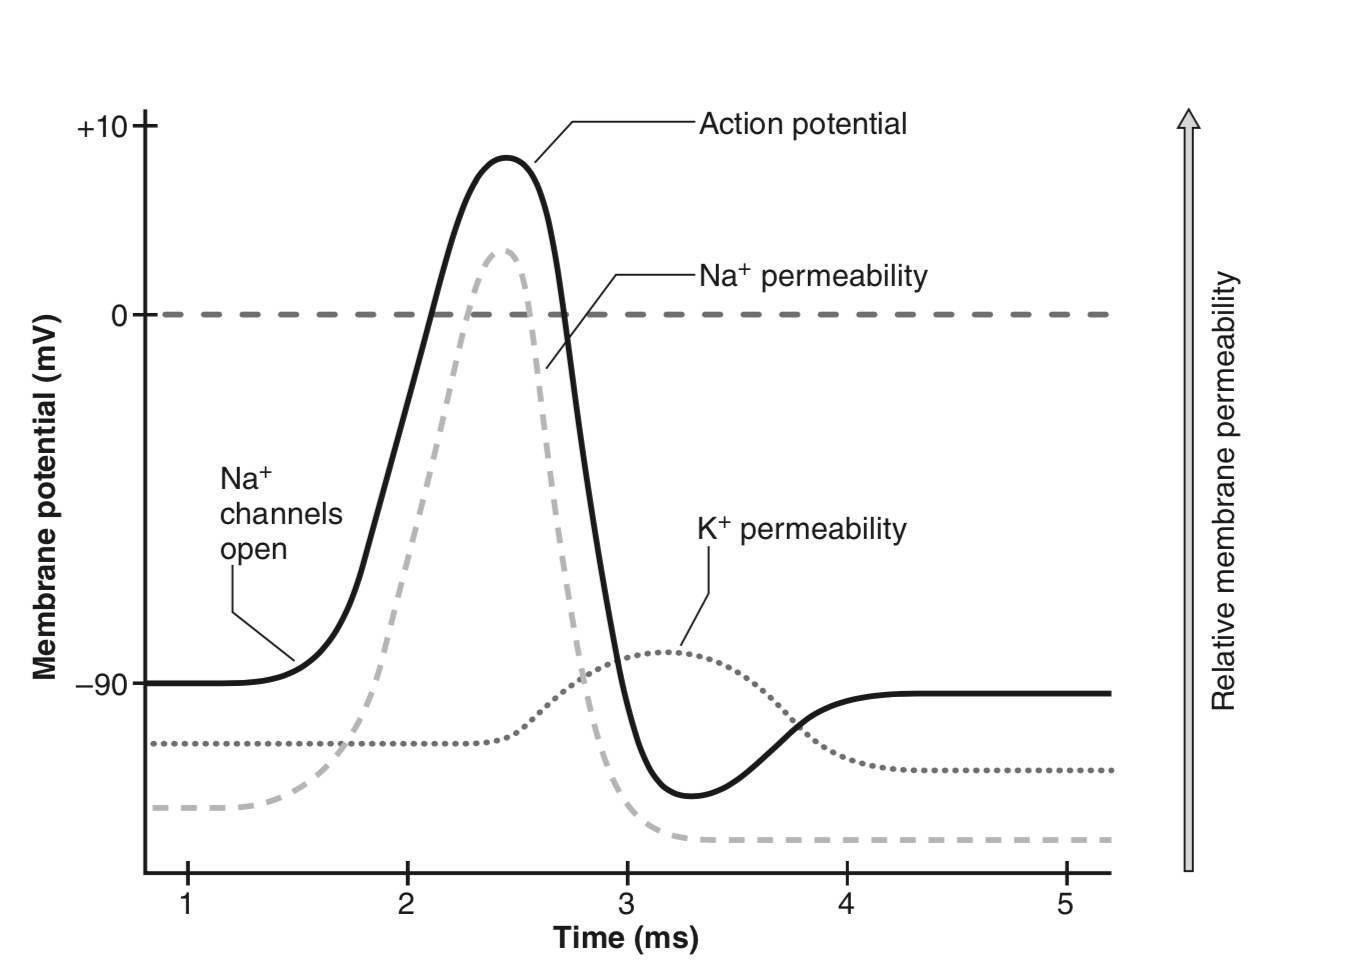
\includegraphics[width=0.75\linewidth]{assets/mfap} 

}

\caption{Time course of a motor action potential (figure from Kamen \& Gabriel, 2010).}\label{fig:mfap}
\end{figure}

The MAP is followed by a \emph{refractory period}, characterised by a
decrease in membrane excitability. This refractory period can be further
decomposed in an \emph{absolute} refractory period during which all
\(\text{Na}^{+}\) channels are closed, and a \emph{relative} refractory
period where some \(\text{Na}^{+}\) channels are open (but to a lesser
extent than before the MAP). Interestingly, this after-impulse
hyperpolarisation limits the frequency of MAPs (Kamen \& Gabriel,
\protect\hyperlink{ref-kamen_essentials_2010}{2010}).

\subsubsection{The motor unit}\label{the-motor-unit}

The \emph{motor unit} is the smallest controllable muscular unit. It
consists in a single \(\alpha\)-motoneuron, its neuromuscular junction,
and all the muscle fibers it innervates. The number of motor units and
their \emph{innervation ratio} (i.e., the number of muscle fibers per
motor unit) can vary by muscle. Because a single motoneuron can
innervate multiple muscle fibers, the firing of a single motoneuron
results in the simultaneous discharge of many muscle fibers. The
\emph{motor unit action potential} (MUAP) is the electric field
resulting from the sum of the electric fields emitted by each fiber of
the motor unit. In other words, it represents the spatiotemporal
summation of individual MAPs originating from muscle fibers that are
sufficiently close to a given electrode. This generates a \emph{train}
of MUAPs, called \emph{motor unit action potential trains} (MUAPTs). The
mixture of MUAPTs coming from different motor units constitute the raw
EMG signal (cf.~Figure \ref{fig:muap}).

\begin{figure}[H]

{\centering 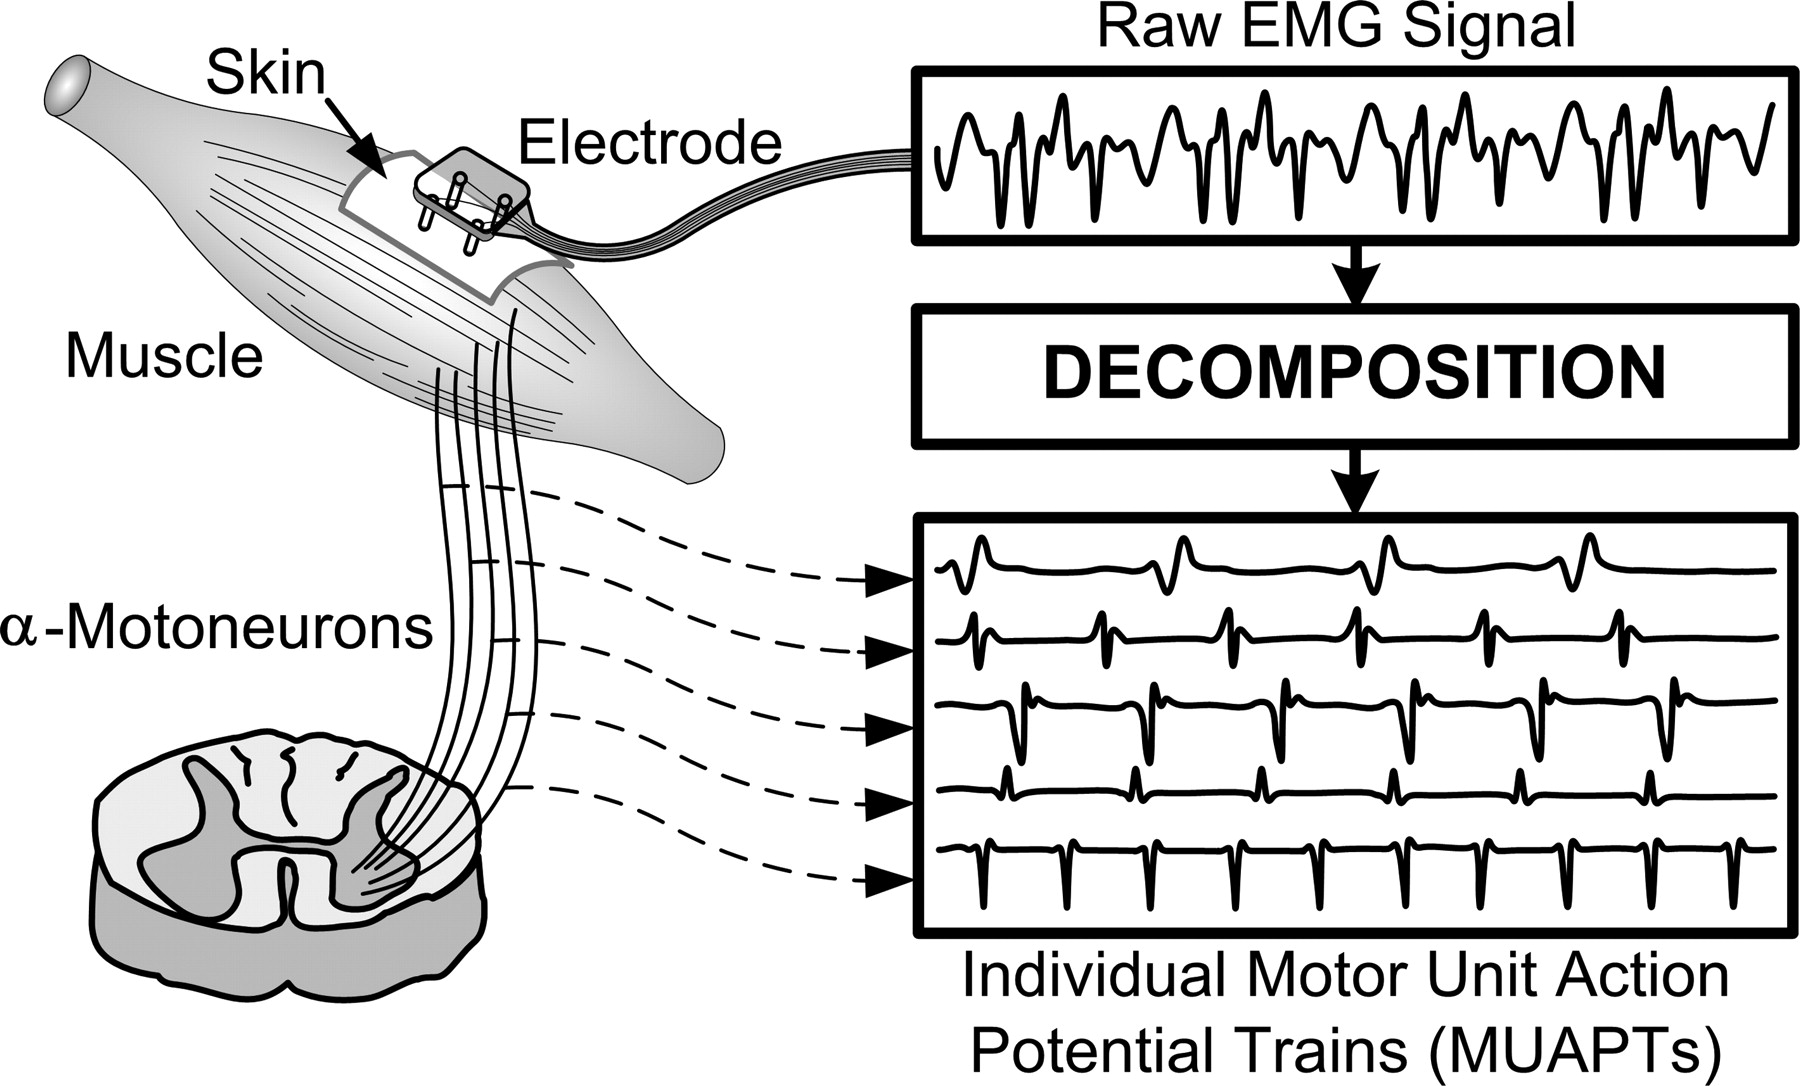
\includegraphics[width=0.75\linewidth]{assets/muap} 

}

\caption{Motor unit action potential representation (Figure from De Luca et al., 2006).}\label{fig:muap}
\end{figure}

To sum up, the EMG signal results from a mixture of recruited motor
units: it is composed of the sum of several to many MUAPTs. This signal
can vary considerably because of factors such as the muscle length
(Babault, Pousson, Michaut, \& Van Hoecke,
\protect\hyperlink{ref-babault_effect_2003}{2003}), the distance between
the muscle fiber (of interest) and the electrode, the fiber length or
the muscle temperature. In the next section, we discuss in more details
how this signal can be acquired.

\subsection{EMG instrumentation and
recording}\label{emg-instrumentation-and-recording}

Myoelectric measurements have a long history, starting in the XVII and
XVIII centuries with the classical observations that muscle contraction
can generate electricity and that electrical impulses can generate
muscle contraction. The term of electromyography and the first EMG
measures were realised at the end of the XIXth century, and the quality
of EMG measurements did not cease to improve since (see Raez, Hussain,
\& Mohd-Yasin, \protect\hyperlink{ref-raez_techniques_2006}{2006}, for a
brief historical perspective).

Two main types of sensors have been used to record EMG signals, varying
by their invasiveness. First, \emph{indwelling} (intramuscular)
recordings can be acquired via electrodes directly inserted into the
muscle. This form of EMG is mostly used in rehabilitation, for diagnosis
of muscle function and to examine nerve conduction (Fridlund \&
Cacioppo, \protect\hyperlink{ref-fridlund_guidelines_1986}{1986}).
Second, \emph{surface electromyography} can be recorded at the surface
of the skin. Each method is associated with its own type of sensors, its
own advantages and disadvantages. Surface electrodes have the advantage
of being easy to use and non-invasive. However, their use is limited to
(large and) superficial muscles. Moreover, because of the phenomenon of
\emph{cross-talk}\footnote{The phenomenon of \emph{cross-talk} can be
  defined as the mixing of the electrical activity of the muscle of
  interest with the electrical activity of adjacent or distant muscles,
  that are not of primary interest.}, it is difficult to isolate the
activity of specific muscles using surface EMG. On the opposite,
intramuscular EMG (that can be recorded via a single needle or two wires
implanted directly into the muscle) are highly selective and can
sometimes record the activity of individual motor units. In addition,
indwelling recordings are not submitted to \emph{tissue filtering}
(i.e., the fact that muscles tissues act as low-pass filters), in
contrast to surface recordings.

In reason of the important intercrossing and superposition of facial
muscles, surface EMG recorded over facial muscles does not generally
represent the activity of a single muscle, but rather a mixture of
muscles activations (De Luca,
\protect\hyperlink{ref-de_luca_use_1997}{1997}; Rapin,
\protect\hyperlink{ref-Rapin2011}{2011}). As a result, it is usually
inappropriate, when using surface EMG, to attribute the recorded
activity to a single muscle (Fridlund \& Cacioppo,
\protect\hyperlink{ref-fridlund_guidelines_1986}{1986}). Whereas for the
sake of simplicity, we designate sensors by the name of the underlying
muscle of interest (e.g., ``FRO'' for the \emph{frontalis} muscle), it
should be kept in mind that these sensors reflect the activity of
``sites'', rather than the activity of single muscles.

Aside from \emph{cross-talk}, many other factors can affect the EMG
signals. These factors are usually described under three main categories
(for more details, see De Luca,
\protect\hyperlink{ref-de_luca_use_1997}{1997}):

\begin{itemize}
\item
  The \emph{causative factors}, that have a basic effect on EMG signals.
  These factors can be further subdivided into two classes: i) the
  \emph{extrinsic} factors, including factors such as the type of
  electrode (e.g., size, shape, placement) or the inter-electrode
  distance and ii) the \emph{intrinsic} factors such as physiological or
  anatomical factors (e.g., fiber type, fiber diameter, blood flow).
\item
  The \emph{intermediate factors}. These are the physiological phenomena
  that are influenced by one or more of the causative factors and that
  in turn influence the deterministic factors, such as the conduction
  velocity, spatial filtering or the signal \emph{cross-talk}.
\item
  Finally, the \emph{deterministic factors} are influenced by the
  intermediate factors and have a direct effect on the EMG signal. These
  include the number of active motor units or the amplitude, duration
  and shape of the MUAPs.
\end{itemize}

All these factors contribute to modulating both the amplitude of the EMG
signal and its spectral properties (e.g., its mean or median frequency).
The importance of these perturbating factors should be acknowledged and
controlled as far as possible. In our work, we use state-of-the art
surface EMG apparatus, specifically developed to tackle these issues, as
well as standardised procedures (more details regarding the EMG
apparatus are provided in chapters 3 to 5).

\subsection{EMG signal processing}\label{emg-signal-processing}

The raw EMG signal is a stochastic train of MUAPs. As put by Fridlund \&
Cacioppo (\protect\hyperlink{ref-fridlund_guidelines_1986}{1986}),
``when heard through a speaker, the raw EMG signal sounds like popcorn
popping''. Therefore, it is usually unsuitable for immediate
quantification. In order to illustrate what the EMG signal looks like,
we simulated EMG data based on a standard algorithm implemented in the
\texttt{biosignalEMG} package (Guerrero \& Macias-Diaz,
\protect\hyperlink{ref-R-biosignalEMG}{2018}). This simulated EMG signal
is represented in Figure \ref{fig:emgplot1}.

\begin{figure}[H]

{\centering 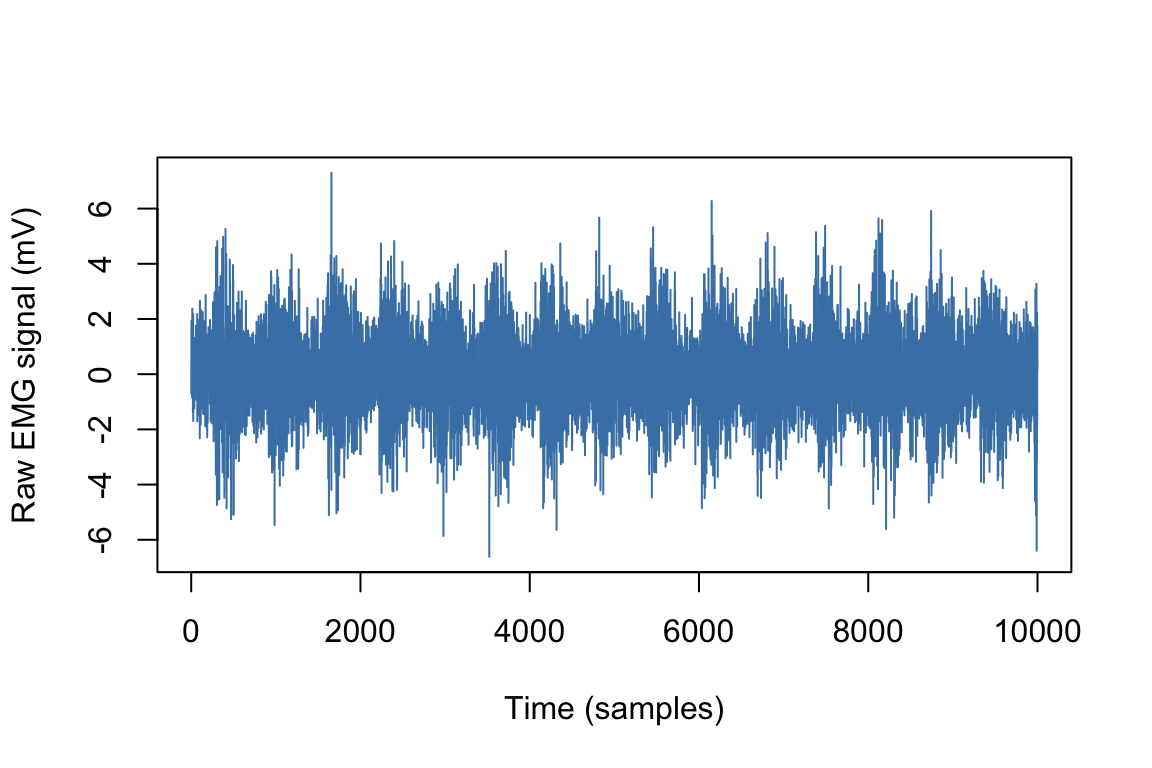
\includegraphics[width=1\linewidth]{02-chap2_files/figure-latex/emgplot1-1} 

}

\caption{Simulated EMG signal.}\label{fig:emgplot1}
\end{figure}

We usually rectify the EMG signal by taking its absolute value and
subtracting the mean in order to correct for any offset (bias) present
in the raw data. The result of this operation is represented in Figure
\ref{fig:emgplot2}.

\begin{figure}[H]

{\centering 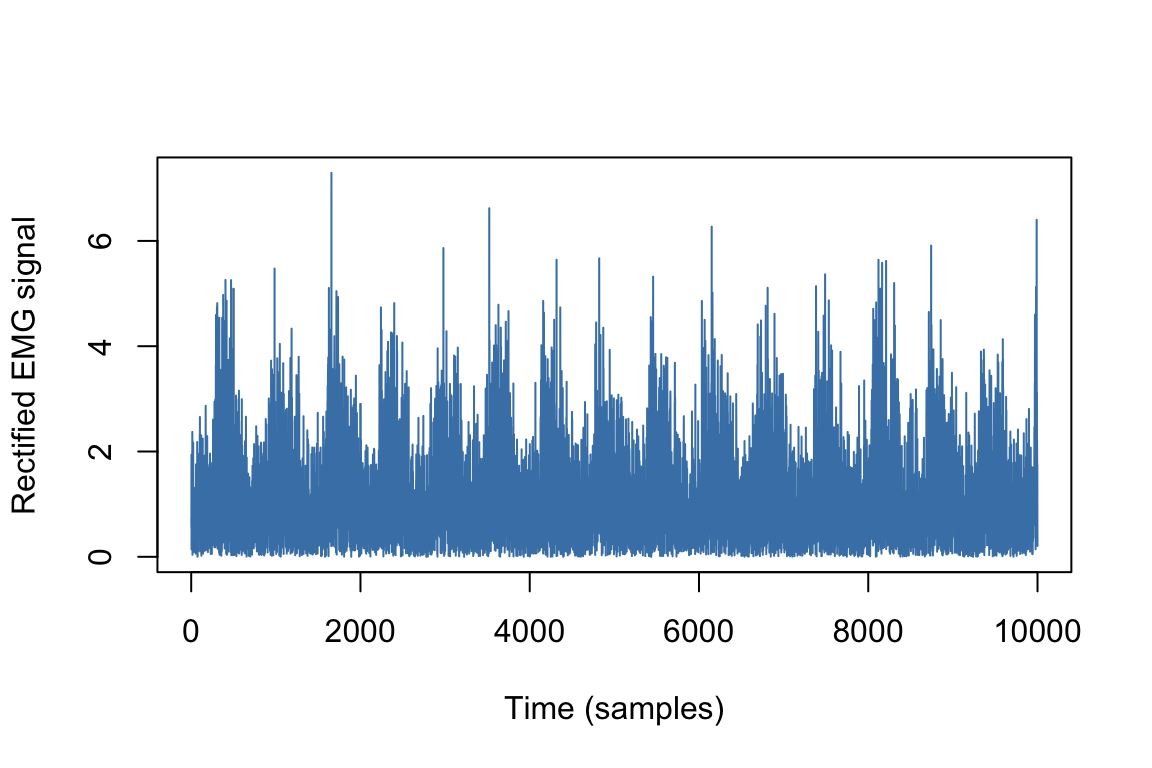
\includegraphics[width=1\linewidth]{02-chap2_files/figure-latex/emgplot2-1} 

}

\caption{Rectified EMG signal.}\label{fig:emgplot2}
\end{figure}

Then, the signal is usually low-pass filtered, with a cut-off frequency
depending on the nature of the study. From there, two main measures can
be used to represent the magnitude of the muscle activity\footnote{But
  see for instance Phinyomark, Nuidod, Phukpattaranont, \& Limsakul
  (\protect\hyperlink{ref-phinyomark_feature_2012}{2012}), for a brief
  overview of other features that can be extracted from the surface EMG
  signal.}. The first one is the \emph{mean absolute value} (MAV), which
is computed over a specific interval and where \(|x_{n}|\) is the
absolute value of a datum of EMG in the data window.

\[MAV = \frac{1}{N} \sum_{n=1}^{N} | x_{n} |\]

The unit of measurement is usually the \(mV\) and the MAV calculation is
generally similar to the numerical formula for integration (Kamen \&
Gabriel, \protect\hyperlink{ref-kamen_essentials_2010}{2010}). The
second one is the \emph{root-mean-square} (RMS) amplitude:

\[RMS = \sqrt{ \frac{1}{N} \sum_{n=1}^{N} x^{2}_{n} }\]

where \(x^{2}_{n}\) is the squared value of each EMG datum and has both
physical and physiological meanings. Put broadly, the RMS it taken to
reflect the level of the physiological activities in the motor unit
during contraction. Both the MAV and the RMS are illustrated in Figure
\ref{fig:emgplot3}.

\begin{figure}[H]

{\centering 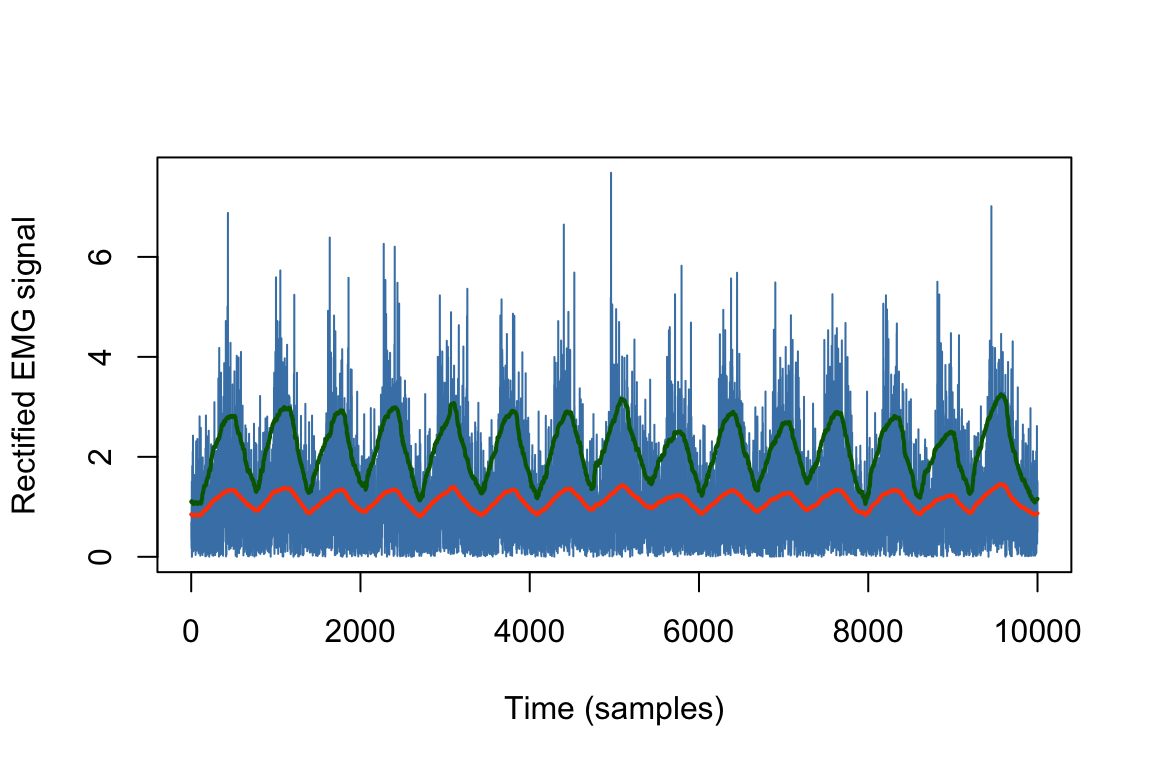
\includegraphics[width=1\linewidth]{02-chap2_files/figure-latex/emgplot3-1} 

}

\caption{Illustration of the MAV (in orange) and RMS (in green) values. These two features are usually highly correlated but differ in magnitude. More precisely, the RMS is proportional to the MAV when the signal has a Gaussian shape.}\label{fig:emgplot3}
\end{figure}

These features provide the \emph{envelope} of the EMG signal and
therefore provide insights about the \emph{amplitude} of the EMG signal.
This envelope can then be summarised (e.g., via its mean or median) over
a period of interest (e.g., during the utterance of some phoneme).

\section{Statistical modelling and statistical
inference}\label{statistical-modelling-and-statistical-inference}

\subsection{Limitations of the standard statistical approach in
Psychology}\label{limitations-of-the-standard-statistical-approach-in-psychology}

Numerous authors have highlighted the limitations inherent to the
Null-Hypothesis Significance Testing (NHST) approach and the (exclusive)
reliance on \emph{p}-values and significance testing (e.g., Bakan,
\protect\hyperlink{ref-bakan_test_1966}{1966}; Gigerenzer,
\protect\hyperlink{ref-Gigerenzer2004}{2004}; Kline,
\protect\hyperlink{ref-Kline2004}{2004}; Lambdin,
\protect\hyperlink{ref-Lambdin2012}{2012}; Meehl,
\protect\hyperlink{ref-meehl_theory-testing_1967}{1967}; Trafimow et
al., \protect\hyperlink{ref-trafimow_manipulating_2018}{2018}).
Considering these limitations, some authors have recommended to push
away significance testing and to develop the use of effect size
estimates and confidence intervals in order to favour accumulation of
evidence and a meta-analytical mode of thinking (e.g., Cumming,
\protect\hyperlink{ref-Cumming2012}{2012},
\protect\hyperlink{ref-cumming_new_2014}{2014}).

However, the apparent superiority of confidence intervals over
\emph{p}-values is an illusion. Indeed, as noted by many observers,
confidence intervals are simply inverted significance tests. In other
words, the confidence interval represents the range of values that are
significant at some \(\alpha\) level. Therefore, compared to a
\emph{p}-value, a confidence interval does not bring \emph{any} new
inferential value. Moreover, its interpretation might be as hard as the
interpretation of \emph{p}-values. For instance, contrary to a widely
shared belief, confidence intervals do not contain the
\((1 - \alpha) \cdot 100\)\% most probable values of the parameter
(e.g., Morey, Hoekstra, Rouder, Lee, \& Wagenmakers,
\protect\hyperlink{ref-morey_fallacy_2015}{2015}; Nalborczyk, Bürkner,
\& Williams, \protect\hyperlink{ref-nalborczyk_pragmatism_2019}{2019}).

That being said, it is fair to acknowledge that using confidence
intervals (instead of or in addition to single \emph{p}-values) do shift
the emphasis from a mechanical (mindless) point-hypothesis testing
procedure to a more careful consideration of the range of values that
are \emph{compatible} with some hypothesis. More importantly, it
emphasises the uncertainty that accompanies every statistical procedure.
Indeed, we think that most of the caveats that are attributed to a
specific statistical procedure (e.g., to NHST) are really caveats of the
way it is used. Namely, the fact that is used in a categorical and
absolute way. This tendency has been coined as \emph{dichotomania}
(i.e., the tendency to consider that results are either present --if
significant-- or absent --if non-significant), or \emph{trichotomania}
(e.g., when considering evidence ratios thresholds).

These biases have been highlighted by many statisticians in the past
(e.g., Wasserstein \& Lazar,
\protect\hyperlink{ref-wasserstein_asas_2016}{2016}). Very recently,
\emph{The American Statistician} published a special issue on
\emph{Moving to a Wold Beyond ``p\textless{}.05''}, with the intention
to provide new recommendations for users of statistics (e.g.,
researchers, policy makers, journalists). This issue comprises 43
original papers aiming to provide new guidelines and practical
alternatives to the mindless use of statistics. In the accompanying
editorial, Wasserstein, Schirm, \& Lazar
(\protect\hyperlink{ref-wasserstein_moving_2019}{2019}) summarise these
recommendations in the form of the ATOM guidelines: ``\textbf{A}ccept
uncertainty. Be \textbf{t}houghtful, \textbf{o}pen, and
\textbf{m}odest.'' We describe below how our statistical approach might
be understood in the light of these core principles.

\begin{itemize}
\item
  \textbf{Accept uncertainty}: we try to represent and to acknowledge
  uncertainty in our analyses and conclusions. For instance, we do not
  conclude and/or infer that an effect is either ``present'' or
  ``absent'', but we report the \emph{estimated} magnitude of the effect
  and the uncertainty that comes with this estimation. Additionally,
  when relevant, we report probabilistic statements based on the
  posterior distribution.
\item
  \textbf{Be thoughtful}: for each analysis opportunity (i.e., for each
  dataset to analyse), we consider what would be the most appropriate
  modelling strategy but we also acknowledge that there is no unique
  best way to analyse a given dataset. In most empirical chapters, we
  clearly distinguish between confirmatory (preregistered) and
  exploratory (non-preregistered) statistical analyses. We routinely
  evaluate the \emph{validity} of the statistical model (and of its
  assumptions) and we are suspicious of statistical \emph{defaults}. We
  try to consider the \emph{practical} significance of the results,
  rather than their \emph{statistical} significance. We use a variety of
  statistics (e.g., effect sizes, interval estimates, information
  criteria) to obtain a more diverse picture of the meaning of the
  results.
\item
  \textbf{Be open}: the soundness of a statistical procedure (and more
  generally, of an inferential procedure) can only be evaluated if it is
  made transparent to peers and readers for critical examination.
  Therefore, we take some space in the next section (but also in each
  experimental chapter) to motivate our statistical modelling decisions.
  We also make all \texttt{R} scripts available to ensure the
  reproducibility of the analyses. We try to be exhaustive in the way we
  report our analyses and we beware of shortcuts than could hinder
  important information to the reader.
\item
  \textbf{Be modest}: we recognise that there is no unique ``true
  statistical model'' and we discuss the limitations of our analyses and
  conclusions. We also recognise that scientific inference is much
  broader than statistical inference (e.g., a degenerative research
  program is much more informative than a non-significant
  \emph{p}-value). We try not to conclude anything from a single study
  without the warranted uncertainty.
\end{itemize}

To sum up, we try to acknowledge the uncertainty that accompanies every
(statistical) inference. In the next section, we present in more details
what our approach does entail and we introduce some key technical
concepts.

\subsection{Our statistical approach}\label{our-statistical-approach}

In brief, we tried to move from the point-hypothesis mechanical testing
to an approach that emphasises parameter estimation, model comparison,
and continuous model expansion (e.g., Cumming,
\protect\hyperlink{ref-Cumming2012}{2012},
\protect\hyperlink{ref-cumming_new_2014}{2014}; Gelman \& Hill,
\protect\hyperlink{ref-gelman_data_2006}{2006}; Gelman et al.,
\protect\hyperlink{ref-gelman_bayesian_2013}{2013}; Judd, McClelland, \&
Ryan, \protect\hyperlink{ref-judd_data_2009}{2009}; Kruschke,
\protect\hyperlink{ref-kruschke_doing_2015}{2015}; Kruschke \& Liddell,
\protect\hyperlink{ref-kruschke_bayesian_2018}{2018}\protect\hyperlink{ref-kruschke_bayesian_2018}{a},
\protect\hyperlink{ref-kruschke_bayesian_2018-1}{2018}\protect\hyperlink{ref-kruschke_bayesian_2018-1}{b};
McElreath, \protect\hyperlink{ref-R-rethinking}{2016}). In other words,
our approach can be defined as a \emph{statistical modelling} approach
rather than a \emph{statistical testing} approach. It means that we try
to \emph{model} the data (or rather the process that generated the
data), rather than to ``test'' it. We carefully consider what could be
the process that generated the data and we try to model it
appropriately. For instance, we do not fit reaction time data, Likert
data, or electromyographic data using the same model, as this practice
would lead to high rates of erroneous inferences.

Throughout this work, we use Bayesian statistical modelling, not by
dogmatism, but because we think the Bayesian approach provides richer
inferences than the frequentist one. The main advantage of the Bayesian
approach is the explicit use of probability to model the uncertainty
(see Box \ref{logic}). By doing so, the Bayesian approach permits to
evaluate the probability of a parameter (or a vector of parameters)
\(\theta\), given a set of data \(y\):

\[p(\theta|y) = \frac{p(y|\theta)p(\theta)}{p(y)}\]

Using this equation (known as Bayes' theorem), a probability
distribution \(p(\theta|y)\) can be derived (called the \emph{posterior
distribution}), that reflects knowledge about the parameter, given the
data and the prior information. This distribution is the goal of any
Bayesian analysis and contains all the information needed for inference.

The term \(p(\theta)\) corresponds to the \emph{prior distribution},
which specifies the prior information about the parameters (i.e., what
is known about \(\theta\) before observing the data) as a probability
distribution. The left hand of the numerator \(p(y|\theta)\) represents
the \emph{likelihood}, also called the \emph{sampling distribution} or
\emph{generative model}, and is the function through which the data
affect the posterior distribution. The likelihood function indicates how
likely the data are to appear, for each possible value of \(\theta\).
Finally, \(p(y)\) is called the \emph{marginal likelihood}. It is meant
to normalise the posterior distribution, that is, to scale it in the
``probability world''. It gives the ``probability of the data'', summing
over all values of \(\theta\) and is described by
\(p(y) = \sum_{\theta} p(\theta) p(y|\theta)\) for discrete parameters,
and by \(p(y) = \int p(\theta) p(y|\theta) d\theta\) in the case of
continuous parameters.

All this pieced together shows that the result of a Bayesian analysis,
namely the posterior distribution \(p(\theta|y)\), is given by the
product of the information contained in the data (i.e., the likelihood)
and the information available before observing the data (i.e., the
prior). This constitutes the crucial principle of Bayesian inference,
which can be seen as an updating mechanism. To sum up, Bayes' theorem
allows a prior state of knowledge to be updated to a posterior state of
knowledge, which represents a compromise between the prior knowledge and
the empirical evidence.

\vspace{2mm}

\begin{mybox}[label = logic]{Probability theory as extended logic}

Probability theory has been argued to be nothing more than \textit{extended logic}. In other words, it generalises the rules of logic that apply to discrete events (e.g., TRUE or FALSE events) to continuous events. By doing this move, probability theory gives a way to represent and to quantify the \textit{uncertainty}. Importantly, the rules of probability have the same status as the rules of logic: these rules can be used to derive statements (conclusions) that are guaranteed to be correct given that some premises are correct.\\

Bayesian statistics can simply be presented as an application of probability theory to statistical analysis. Whereas the dependence of the inferential conclusions on prior assumptions is sometimes presented as a downside of this type of analysis, it is precisely what makes them \textit{optimal} or \textit{coherent} (in the sense of respecting the rules of probability). As put by Vandekerckhove (2018), the claim that Bayesian methods would be invalidated by their reliance on prior assumptions would be akin to conclude that logical deductions are somehow invalidated because they depend on premises.

\end{mybox}

We also use \emph{multilevel models} (also known as \emph{mixed-models})
to handle complex dependency structures and to obtain more precise
estimates. A more accurate description of Bayesian multilevel models is
outside the scope of this introductory section but the interested reader
is redirected toward several existing tutorial papers (e.g., Nalborczyk,
Batailler, Lœvenbruck, Vilain, \& Bürkner,
\protect\hyperlink{ref-nalborczyk_introduction_2019}{2019}; Nicenboim \&
Vasishth, \protect\hyperlink{ref-nicenboim_statistical_2016}{2016};
Sorensen, Hohenstein, \& Vasishth,
\protect\hyperlink{ref-sorensen_bayesian_2016}{2016}). Throughout this
work, we also make use of several tools with very distinct properties
and uses. For instance, we use Bayes factors (BFs) to quantify the
relative evidence for a statistical hypothesis (see Box \ref{BF}), we
use information criteria to assess the predictive abilities of our
models (see Box \ref{IC}), we use posterior predictive checks as well as
a diagnostics tools (e.g., convergence indexes, trace plots) to assess
the validity of our models, and we use summary statistics when
appropriate to convey the meaning of the main results.

\vspace{2mm}

\begin{mybox}[label = BF]{What is a Bayes factor ?}

It is a rule in statistics that every statistics has already been suggested as the \textit{new statistics}. Confidence intervals have been suggested as a replacement to \textit{p}-values, being purportedly more informative and less difficult to interpret. Credible intervals have been suggested as a replacement to confidence intervals, for roughly the same reasons. Bayesian hypothesis testing through Bayes factors (BFs) has also been suggested as a replacement for frequentist hypothesis testing. It has been argued that they permit a richer inference and that they come with a more straightforward interpretation. Whereas this might be true, they nonetheless come with their lot of misinterpretations.\\

To highlight what BFs are and what they are not, it might be useful to write down the formula used to compute them. To this end, it is useful to write the Bayes rule in its \textit{odds form}, making the BF explicitly visible:

$$\underbrace{\dfrac{p(H_{0}|D)}{p(H_{1}|D)}}_{posterior\ odds} = \underbrace{\dfrac{p(D|H_{0})}{p(D|H_{1})}}_{Bayes\ factor} \times \underbrace{\dfrac{p(H_{0})}{p(H_{1})}}_{prior\ odds}$$

This equation reveals that the \textit{posterior odds}, the ratio of the posterior probability (i.e., how much more probable is hypothesis 1 ($H_{1}$) as compared to hypothesis 2 ($H_{2}$), after seeing the data $D$), is equal to the ratio of the probability of the data given the first hypothesis and the probability of the data given the second hypothesis, multiplied by the \textit{prior odds} (i.e., how much more probable was hypothesis 1 ($H_{1}$) as compared to hypothesis 2 ($H_{2}$), before seeing the data $D$).\\ 

Importantly, what we consider as \textit{evidence} in the Bayesian framework is also known as a \textit{marginal likelihood} and represents the information contained in the data, weighted by the prior information. It is a sum when parameters are discrete or an integral when parameters are continuous.

$$\text{evidence}\ = p(D|H) = \int p(\theta|H) p(D|\theta,H) \text{d}\theta$$

Therefore, the BF does not indicate how much "probable" a hypothesis is, or how much more probable a hypothesis is, compared to another one (this would be to conflate the BF with the posterior odds). Instead, the BF can be (should be) interpreted either i) as a ratio of two \textit{marginal likelihoods} (i.e., a ratio of \textit{evidence}) or ii) as an updating factor, indicating how we should reallocate credibility from prior knowledge (what we knew before seeing the data) to posterior knowledge (what we know after seeing the data).

\end{mybox}

Bayes factors are often said to have desirable \emph{asymptotic} (i.e.,
when the number of observations is very large) properties. Indeed, they
are \emph{consistent} for model identification. It means that if a
``true'' statistical model is in the set of models that are compared,
using a BF will usually lead to selecting this ``true'' model with a
probability approaching 1 with increasing sample size. Whereas this
seems as an appealing property or not depends on the underlying
statistical philosophy. Indeed, one could question whether it is
sensible to assume a ``true model'' (an oxymoron) in real life,
especially in the social sciences (e.g., Burnham \& Anderson,
\protect\hyperlink{ref-burnham_model_2002}{2002},
\protect\hyperlink{ref-burnham_multimodel_2004}{2004}). As Findley
(\protect\hyperlink{ref-findley_unbiasedness_1985}{1985}) notes:
\emph{``{[}\ldots{}{]} consistency can be an undesirable property in the
context of selecting a model''}. A more realistic question is then not
to look for the ``true'' model, but rather for the \emph{best} model for
some practical purpose.

The usefulness of information criteria comes from them being
approximations of the \emph{out-of-sample deviance} (see Box \ref{IC}).
In the present PhD work, we used generalisations of the AIC (especially
the WAIC and LOOIC) that also approximate the \emph{out-of-sample
deviance} and as such give an indication of how good/bad a model is to
predict future (i.e., non-observed) data.

\vspace{2mm}

\begin{mybox}[label = IC]{Information criteria}

Hirotugu Akaike noticed that the negative log-likelihood of a model + 2 times its number of parameters was approximately equal to the \textbf{out-of-sample deviance} of a model, which lead to what is nowadays famously known as the \textit{Akaike information criterion} (AIC):

$$\text{AIC} = \underbrace{\underbrace{-2\log(\mathcal{L}(\hat{\theta}|\text{data}))}_{\text{in-sample deviance}} + 2K}_{\approx\ \text{out-of-sample deviance}}$$

where $K$ is the number of parameters of the model and the \textit{deviance} is a measure of discrepancy between the data and the model. Interestingly, we can make a distinction between two types of deviances.\\

First, the \textbf{in-sample deviance} indicates how bad a model is to explain the current dataset (the dataset used to fit the model). Second, and more importantly, the \textbf{out-of-sample deviance} indicates how bad a model is to explain a \textbf{future} dataset issued from the same data generation process (the same population).

\end{mybox}

In brief, in the present work, we used various methods but coherently
with a few (nuanced) guiding principles. Namely, we favoured a
\emph{model comparison} approach (e.g., Burnham \& Anderson,
\protect\hyperlink{ref-burnham_model_2002}{2002},
\protect\hyperlink{ref-burnham_multimodel_2004}{2004}; Judd et al.,
\protect\hyperlink{ref-judd_data_2009}{2009}), we used several
statistics when they provide complementary information (e.g., using both
posterior probabilities, information criteria or BFs), we assessed the
validity of our models (e.g., via posterior predictive checks), we
reported these analyses transparently, and we tried to convey
uncertainty in our conclusions.

\section{Overview of the following
chapters}\label{overview-of-the-following-chapters}

The experiments ran during this PhD will be presented as five empirical
chapters that can be grouped under two main axes. In the first couple of
experiments, we used surface electromyography and muscle-specific
relaxation to investigate the involvement of the speech motor system
during induced verbal and non-verbal rumination (Chapter 3 \& 4). In
Chapter 5, we used surface electromyography and machine learning
algorithms to decode the muscle-specific EMG correlates of inner speech
production. In the last couple of experiments, we switched strategy from
the ``correlates strategy'' to the ``interference strategy'', where the
goal was to directly interfere with the activity of the speech motor
system. More precisely, we used articulatory suppression to disrupt
induced rumination in Chapter 6, and we used articulatory suppression to
disrupt either induced rumination or problem-solving in Chapter 7.
Finally, in Chapter 8, we summarise the main findings, discuss their
implications and suggest ways forward from both a theoretical and an
experimental perspective.

\part{Experimental
chapters}\label{part-experimental-chapters}

\chapter{Orofacial electromyographic correlates of induced verbal
rumination}\label{orofacial-electromyographic-correlates-of-induced-verbal-rumination}

\initial{A}dd a summary of the research and brief introduction to this
first empirical chapter here\ldots{}\footnote{This experimental chapter
  is a published paper reformatted for the need of this thesis. Source:
  Nalborczyk, L., Perrone-Bertolotti, M., Baeyens, C., Grandchamp, R.,
  Polosan, M., Spinelli, E., \ldots{} L\oe venbruck, H. (2017).
  Orofacial Electromyographic Correlates of Induced Verbal Rumination.
  \emph{Biological Psychology, 127}, 53-63.
  \url{https://dx.doi.org/10.1016/j.biopsycho.2017.04.013}.}

\section{Abstract}\label{abstract-1}

Rumination is predominantly experienced in the form of repetitive verbal
thoughts. Verbal rumination is a particular case of inner speech.
According to the \emph{Motor Simulation view}, inner speech is a kind of
motor action, recruiting the speech motor system. In this framework, we
predicted an increase in speech muscle activity during rumination as
compared to rest. We also predicted increased forehead activity,
associated with anxiety during rumination. We measured electromyographic
activity over the \emph{orbicularis oris superior and inferior},
\emph{frontalis} and \emph{flexor carpi radialis} muscles. Results
showed increased lip and forehead activity after rumination induction
compared to an initial relaxed state, together with increased
self-reported levels of rumination. Moreover, our data suggest that
orofacial relaxation is more effective in reducing rumination than
non-orofacial relaxation. Altogether, these results support the
hypothesis that verbal rumination involves the speech motor system, and
provide a promising psychophysiological index to assess the presence of
verbal rumination.

\section{Introduction}\label{introduction}

As humans, we spend a considerable amount of time reflecting upon
ourselves, thinking about our own feelings, thoughts and behaviors.
Self-reflection enables us to create and clarify the meaning of past and
present experiences (Boyd \& Fales,
\protect\hyperlink{ref-boyd_reflective_1983}{1983}; Nolen-Hoeksema,
Wisco, \& Lyubomirsky,
\protect\hyperlink{ref-Nolen-Hoeksema2008}{2008}). However, this process
can lead to unconstructive consequences when self-referent thoughts
become repetitive, abstract, evaluative, and self-critical (Watkins,
\protect\hyperlink{ref-Watkins2008}{2008}).

Indeed, rumination is most often defined as a repetitive and recursive
mode of responding to negative affect (Rippere,
\protect\hyperlink{ref-Rippere1977}{1977}) or life situations (M. S.
Robinson \& Alloy, \protect\hyperlink{ref-Robinson2003}{2003}). Although
rumination is a common process that can be observed in the general
population (Watkins, \protect\hyperlink{ref-Watkins2008}{2008}), it has
been most extensively studied in depression and anxiety. Depressive
rumination has been thoroughly studied by Susan Nolen-Hoeksema, who
developed the Response Style Theory (RST, Nolen-Hoeksema,
\protect\hyperlink{ref-nolen-hoeksema_responses_1991}{1991}). According
to the RST, depressive rumination is characterized by an evaluative
style of processing that involves recurrent thinking about the causes,
meanings, and implications of depressive symptoms. Even though
rumination can involve several modalities (i.e., visual, sensory), it is
a predominantly verbal process (Goldwin \& Behar,
\protect\hyperlink{ref-goldwin_concreteness_2012}{2012}; McLaughlin,
Borkovec, \& Sibrava,
\protect\hyperlink{ref-mclaughlin_effects_2007}{2007}). In this study,
we focus on verbal rumination, which can be conceived of as a
particularly significant form of inner speech.

Inner speech or covert speech can be defined as silent verbal production
in one's mind or the activity of silently talking to oneself (Zivin,
\protect\hyperlink{ref-zivin_development_1979}{1979}). The nature of
inner speech is still a matter of theoretical debate (for a review, see
Perrone-Bertolotti et al.,
\protect\hyperlink{ref-Perrone-Bertolotti2014}{2014}). Two opposing
views have been proposed in the literature: the \emph{Abstraction view}
and the \emph{Motor Simulation view}. The \emph{Abstraction view}
describes inner speech as unconcerned with articulatory or auditory
simulations and as operating on an amodal level. It has been described
as ``condensed, abbreviated, disconnected, fragmented, and
incomprehensible to others'' (Vygotsky,
\protect\hyperlink{ref-vygotsky_collected_1987}{1987}). It has been
argued that important words or grammatical affixes may be dropped in
inner speech (Vygotsky,
\protect\hyperlink{ref-vygotsky_collected_1987}{1987}) or even that the
phonological form or representation of inner words may be incomplete (G.
S. Dell \& Repka, \protect\hyperlink{ref-dell_errors_1992}{1992};
Sokolov, \protect\hyperlink{ref-sokolov_inner_1972}{1972}). MacKay
(\protect\hyperlink{ref-mackay_constraints_1992}{1992}) stated that
inner speech is nonarticulatory and nonauditory and that ``Even the
lowest level units for inner speech are highly abstract'' (p.122).

In contrast with this \emph{Abstraction view}, the physicalist or
embodied view considers inner speech production as mental simulation of
overt speech production. As such, it can be viewed as similar to overt
speech production, except that the motor execution process is blocked
and no sound is produced (Gr�zes \& Decety,
\protect\hyperlink{ref-grzes_functional_2001}{2001}; Postma \&
Noordanus, \protect\hyperlink{ref-postma_production_1996}{1996}). Under
this \emph{Motor Simulation view}, a continuum exists between overt and
covert speech, in line with the continuum drawn by Decety \& Jeannerod
(\protect\hyperlink{ref-decety_mentally_1996}{1996}) between imagined
and actual actions. This hypothesis has led certain authors to claim
that inner speech by essence should share features with speech motor
actions (Feinberg,
\protect\hyperlink{ref-feinberg_efference_1978}{1978}; Jones \&
Fernyhough, \protect\hyperlink{ref-Jones2007}{2007}). The \emph{Motor
Simulation view} is supported by several findings. First, covert and
overt speech have comparable physiological correlates: for instance,
measurements of speaking rate(Landauer, 1962) and respiratory rate (B.
Conrad \& Schönle, \protect\hyperlink{ref-conrad_speech_1979}{1979}) are
similar in both. A prediction of the \emph{Motor Simulation view} is
that the speech motor system should be recruited during inner speech.
Subtle muscle activity has been detected in the speech musculature using
electromyography (EMG) during verbal mental imagery, silent reading,
silent recitation (Jacobson,
\protect\hyperlink{ref-jacobson_electrical_1931}{1931}; Livesay, Liebke,
Samaras, \& Stanley, \protect\hyperlink{ref-livesay_covert_1996}{1996};
McGuigan \& Dollins,
\protect\hyperlink{ref-mcguigan_patterns_1989}{1989}; Sokolov,
\protect\hyperlink{ref-sokolov_inner_1972}{1972}), and during auditory
verbal hallucination in patients with schizophrenia (Rapin, Dohen,
Polosan, Perrier, \& Lœvenbruck,
\protect\hyperlink{ref-Rapin2013}{2013}). Second, it has been shown that
covert speech production involves a similar cerebral network as that of
overt speech production. Covert and overt speech both recruit essential
language areas in the left hemisphere (for a review, see
Perrone-Bertolotti et al.,
\protect\hyperlink{ref-Perrone-Bertolotti2014}{2014}). However, there
are differences. Consistent with the \emph{Motor Simulation view} and
the notion of a continuum between covert and overt speech, overt speech
is associated with more activity in motor and premotor areas than inner
speech (e.g., Palmer et al.,
\protect\hyperlink{ref-palmer_event-related_2001}{2001}). This can be
related to the absence of articulatory movements during inner verbal
production. In a reciprocal way, inner speech involves cerebral areas
that are not activated during overt speech (Basho, Palmer, Rubio,
Wulfeck, \& Müller, \protect\hyperlink{ref-basho_effects_2007}{2007}).
Some of these activations (cingulate gyrus and superior rostral frontal
cortex) can be attributed to the inhibition of overt responses.

These findings suggest that the processes involved in overt speech
include those required for inner speech (except for inhibition). Several
studies in patients with aphasia support this view: overt speech loss
can either be associated with an impairment in inner speech (e.g.,
Levine, Calvanio, \& Popovics,
\protect\hyperlink{ref-levine_language_1982}{1982}; Martin \& Caramazza,
\protect\hyperlink{ref-martin_short-term_1982}{1982}) or with intact
inner speech: only the later phases of speech production (execution)
being affected by the lesion (A. D. Baddeley \& Wilson,
\protect\hyperlink{ref-baddeley_phonological_1985}{1985}; Marshall,
Rappaport, \& Garcia-Bunuel,
\protect\hyperlink{ref-marshall_self-monitoring_1985}{1985}; Vallar \&
Cappa, \protect\hyperlink{ref-vallar_articulation_1987}{1987}). Geva,
Bennett, Warburton, \& Patterson
(\protect\hyperlink{ref-geva_discrepancy_2011}{2011}) have reported a
dissociation that goes against this view, however. In three patients
with chronic post-stroke aphasia (out of 27 patients), poorer homophone
and rhyme judgement performance was in fact observed in covert mode
compared with overt mode. A limitation of this study, though, was that
the task was to detect rhymes in written words, which could have been
too difficult for the patients. To overcome this limitation,
Langland-Hassan, Faries, Richardson, \& Dietz
(\protect\hyperlink{ref-langland-hassan_inner_2015}{2015}) have tested
aphasia patients with a similar task, using images rather than written
words. They also found that most patients performed better in the overt
than in the covert mode. They inferred from these results that inner
speech might be more demanding in terms of cognitive and linguistic
load, and that inner speech may be a distinct ability, with its own
neural substrates. We suggest an alternative interpretation to this
dissociation. According to our view, rhyme and homophone judgements rely
on auditory representations of the stimuli (e.g., Paulesu, Frith, \&
Frackowiak, \protect\hyperlink{ref-paulesu_neural_1993}{1993}). Overt
speech provides a strong acoustic output that is fed back to the
auditory cortex and can create an auditory trace, which can be used to
monitor speech. In the covert mode, the auditory output is only mentally
simulated, and its saliency in the auditory system is lesser than in the
overt mode. This is in accordance with the finding that inner speech is
associated with reduced sensory cortex activation compared with overt
speech (Shuster \& Lemieux,
\protect\hyperlink{ref-shuster_fmri_2005}{2005}). In patients with
aphasia, the weakened saliency of covert auditory signals may be
accentuated for two reasons: first, because of impairment in the
motor-to-auditory transformation that produces the auditory simulation,
and second, because of associated auditory deficits. Therefore,
according to our view, the reduced performance observed in rhyme and
homophone judgement tasks in the covert compared with the overt mode in
brain-injured patients, simply indicates a lower saliency of the
auditory sensations evoked during inner speech compared with the actual
auditory sensations fed back during overt speech production. In summary,
these findings suggest that overt and covert speech share common
subjective, physiological and neural correlates, supporting the claim
that inner speech is a motor simulation of overt speech.

However, the \emph{Motor Simulation view} has been challenged by several
experimental results. Examining the properties of errors during the
production of tongue twisters, Oppenheim \& Dell
(\protect\hyperlink{ref-oppenheim_motor_2010}{2010}) showed that speech
errors display a lexical bias in both overt and inner speech. According
to these researchers, errors also display a phonemic similarity effect
(or articulatory bias), a tendency to exchange phonemes with common
articulatory features, but this second effect is only observed with
overt speech or with inner speech accompanied with mouthing. This has
led Oppenheim \& Dell
(\protect\hyperlink{ref-oppenheim_motor_2010}{2010}) to claim that inner
speech is fully specified at the lexical level, but that it is
impoverished at lower featural (articulatory) levels. This claim,
related to the \emph{Abstraction view}, is still debated however, as a
phonemic similarity effect has been found by Corley, Brocklehurst, \&
Moat (\protect\hyperlink{ref-corley_error_2011}{2011}). Their findings
suggest that inner speech is in fact specified at the articulatory
level, even when there is no intention to articulate words overtly.
Other findings however, may still challenge the Motor Simulation view.
Netsell, Ashley, \& Bakker
(\protect\hyperlink{ref-netsell_inner_2010}{2010}) have examined covert
and overt speech in persons who stutter (PWS) and typical speakers. They
have found that PWS were faster in covert than in overt speech while
typical speakers presented similar overt and covert speech rates. This
can be interpreted in favour of the \emph{Abstraction view}, in which
inner representations are not fully specified at the articulatory level,
which would explain why they are not disrupted in PWS speech.
Altogether, these results suggest that full articulatory specification
may not always be necessary for inner speech to be produced.

The aim of this study is to examine the physiological correlates of
verbal rumination in an attempt to provide new data in the debate
between motor simulation and abstraction. A prediction of the
\emph{Motor Simulation view} is that verbal rumination, as a kind of
inner speech, should be accompanied with activity in speech-related
facial muscles, as well as in negative emotion or anxiety-related facial
muscles, but should not involve non-facial muscles (such as arm
muscles). Alternatively, the \emph{Abstraction view} predicts that
verbal rumination should be associated with an increase in
emotion-related facial activity, without activity in speech-related
muscles and non-facial muscles.

There is strong interest in the examination of physiological correlates
of rumination as traditional assessment of rumination essentially
consists of self-reported measures. The measurement of rumination as
conceptualized by Nolen-Hoeksema
(\protect\hyperlink{ref-nolen-hoeksema_responses_1991}{1991}) was
operationalized by the development of the Ruminative Response Scale
(RRS), which is a subscale of the response style questionnaire
(Nolen-Hoeksema \& Morrow,
\protect\hyperlink{ref-nolen-hoeksema_prospective_1991}{1991}). The RRS
consists of 22 items that describe responses to dysphoric mood that are
self-focused, symptom-focused, and focused on the causes and
consequences of one's mood. Based on this scale, Treynor, Gonzalez, \&
Nolen-Hoeksema (\protect\hyperlink{ref-treynor_rumination_2003}{2003})
have offered a detailed description of rumination styles and more
recently, Watkins (\protect\hyperlink{ref-Watkins2008}{2008}) has
further characterized different modes of rumination. The validity of
these descriptions is nevertheless based on the hypothesis that
individuals have direct and reliable access to their internal states.
However, self-reports increase reconstruction biases (e.g., Brewer,
\protect\hyperlink{ref-rubin_what_1986}{1986}; Conway,
\protect\hyperlink{ref-conway_autobiographical_1990}{1990}) and it is
well known that participants have a very low level of awareness of the
cognitive processes that underlie and modulate complex behaviors
(Nisbett \& Wilson, \protect\hyperlink{ref-nisbett_telling_1977}{1977}).

In order to overcome these difficulties, some authors have attempted to
quantify state rumination and trait rumination more objectively, by
recording physiological or neuroanatomical correlates of rumination (for
a review, see Siegle \& Thayer,
\protect\hyperlink{ref-papageorgiou_physiological_2003}{2003}).
Peripheral physiological manifestations (e.g., pupil dilation, blood
pressure, cardiac rhythm, cardiac variability) have been examined during
induced or chronic rumination. Vickers \& Vogeltanz-Holm
(\protect\hyperlink{ref-vickers_effects_2003}{2003}) have observed an
increase in systolic blood pressure after rumination induction,
suggesting the involvement of the autonomic nervous system in
rumination. Moreover, galvanic skin response has shown to be increased
after a rumination induction, in highly anxious women (Sigmon, Dorhofer,
Rohan, \& Boulard, \protect\hyperlink{ref-sigmon_impact_2000}{2000}).
According to Siegle \& Thayer
(\protect\hyperlink{ref-papageorgiou_physiological_2003}{2003}),
disrupted autonomic activity could provide a reliable physiological
correlate of rumination. In this line, Key, Campbell, Bacon, \& Gerin
(\protect\hyperlink{ref-Key2008}{2008}) have observed a diminution of
the high-frequency component of heart rate variability (HF-HRV) after
rumination induction in people with a low tendency to ruminate (see also
Woody, McGeary, \& Gibb,
\protect\hyperlink{ref-woody_brooding_2014}{2014}). A consistent link
between perseverative cognition and decreased HRV was also found in a
meta-analysis conducted by Ottaviani et al.
(\protect\hyperlink{ref-Ottaviani2015}{2015}). Based on these positive
results and on suggestions that labial EMG activity may accompany inner
speech and therefore rumination, our aim was to examine facial EMG as a
potential correlate of rumination and HRV as an index to examine
concurrent validity.

In addition to labial muscular activity, we also recorded forehead
muscular activity (i.e., \emph{frontalis} muscle) because of its
implication in prototypical expression of sadness (e.g., Ekman \&
Friesen, \protect\hyperlink{ref-ekman_facial_1978}{1978}; Kohler et al.,
\protect\hyperlink{ref-kohler_differences_2004}{2004}), reactions to
unpleasant stimuli (Jäncke, Vogt, Musial, Lutz, \& Kalveram,
\protect\hyperlink{ref-Jancke1996}{1996}), and anxiety or negative
emotional state (A. Conrad \& Roth,
\protect\hyperlink{ref-conrad_muscle_2007}{2007})\footnote{The
  \emph{corrugator supercilii} was another potential site, as it is
  sensitive to negative emotions. However, it has been claimed to be
  mostly activated for strong emotions such as fear/terror, anger/rage
  and sadness/grief (Ekman \& Friesen,
  \protect\hyperlink{ref-ekman_facial_1978}{1978}; Sumitsuji, Matsumoto,
  Tanaka, Kashiwagi, \& Kaneko,
  \protect\hyperlink{ref-sumitsuji_electromyographic_1967}{1967}). The
  rumination induction used in this study was designed to have
  participants self-reflect and brood over their failure at the I.Q.
  test. It was not meant to induce such strong emotions. Several studies
  have reported increased activity in the \emph{frontalis} muscle at
  rest in anxious or generalized anxiety disorder patients (for a
  review, see A. Conrad \& Roth,
  \protect\hyperlink{ref-conrad_muscle_2007}{2007}). We expected the
  type of emotional state induced by rumination to be closer to anxiety
  or worry than to strong emotions like fear, anger or grief. It was
  therefore more appropriate to record non-speech facial activity in the
  \emph{frontalis} rather than in the \emph{corrugator.}}. Our
hypothesis was that \emph{frontalis} activity could be an accurate
electromyographic correlate of induced rumination, as a negatively
valenced mental process.

In this study, we were also interested in the effects of relaxation on
induced rumination. Using a relaxation procedure targeted on muscles
involved in speech production is a further way to test the reciprocity
of the link between inner speech (verbal rumination) and orofacial
muscle activity. If verbal rumination is a kind of action, then its
production should be modulated in return by the effects of relaxation on
speech effectors. This idea is supported by the results of (among
others) Cefidekhanie, Savariaux, Sato, \& Schwartz
(\protect\hyperlink{ref-cefidekhanie_interaction_2014}{2014}), who have
observed substantial perturbations of inner speech production while
participants had to realize forced movements of the articulators.

In summary, the current study aimed at evaluating the \emph{Motor
Simulation view} and the \emph{Abstraction view} by using objective and
subjective measures of verbal rumination. To test the involvement of the
orofacial motor system in verbal rumination, we used two basic
approaches. In the first approach, we induced verbal rumination and
examined concurrent changes in facial muscle activity (Experiment 1). In
the second approach, we examined whether orofacial relaxation would
reduce verbal rumination levels (Experiment 2). More specifically, in
Experiment 1, we aimed to provide an objective assessment of verbal
rumination using quantitative physiological measures. Thus, we used EMG
recordings of muscle activity during rumination, focusing on the
comparison of speech-related (i.e., two lip muscles − \emph{orbicularis
oris superior} and \emph{orbicularis oris inferior}) and
speech-unrelated (i.e., forehead −\emph{frontalis}- and forearm −
\emph{flexor carpi radialis}) muscles. Under the \emph{Motor Simulation
view}, an increase in lip and forehead EMG activity should be observed
after rumination induction, with no change in forearm EMG activity,
associated with an increase in self-reported rumination. Alternatively,
under the \emph{Abstraction view}, an increase in forehead activity
should be observed, associated with an increase in self-reported
rumination, and no changes in either lip or forearm activity should be
noted.

In Experiment 2, in order to assess the reciprocity of the rumination
and orofacial motor activity relationship, we evaluated the effects of
orofacial relaxation on rumination. More specifically, we compared three
kinds of relaxation: i) Orofacial Relaxation (i.e., lip muscles), ii)
Arm Relaxation (i.e., to differentiate effects specific to
speech-related muscle relaxation) and iii) Story Relaxation (i.e., to
differentiate effects specific to attentional distraction). If the
\emph{Motor simulation view} is correct, we predicted a larger decrease
of lip and forehead muscle activity after an Orofacial Relaxation than
after an Arm Relaxation (associated with a larger decrease in
self-reported rumination), which should also be larger than after
listening to a story. We also predicted that forearm activity should
remain stable across the three conditions (i.e., should not decrease
after relaxation). Alternatively, if the \emph{Abstraction view} is
correct, we predicted that none of the relaxation conditions should have
an effect on lip or arm activity, because none of these should have
increased after induction. However, we expected to observe a decrease in
forehead activity and self-reported rumination after Orofacial or Arm
relaxation, this decrease being larger than after listening to a Story.
Importantly, we predicted that, under the \emph{Abstraction View} no
superiority of the Orofacial relaxation should be observed over the Arm
relaxation.

\section{Methods}\label{methods}

\subsection{Participants}\label{participants}

Because of the higher prevalence of rumination in women than in men (see
Johnson \& Whisman, \protect\hyperlink{ref-Johnson2013}{2013}, for a
recent meta-analysis), we chose to include female participants only.
Seventy-two female undergraduate students from Univ. Grenoble Alpes,
native French speaking, participated in our study. One participant
presenting aberrant data (probably due to inadequate sensor sticking)
was removed from analyses. Final sample consisted of seventy-one
undergraduate female students (M\textsubscript{age} = 20.58,
SD\textsubscript{age} = 4.99). They were recruited by e-mail diffusion
lists and participated in the experiment for course credits. They did
not know the goals of the study. The cover story presented the research
as aiming at validating a new I.Q. test, more sensitive to personality
profiles. Participants reported having no neurologic or psychiatric
medical history, no language disorder, no hearing deficit, and taking no
medication. Each participant gave written consent and this study has
been approved by the local ethical committee (CERNI, N° 2015-03-03-61).

\subsection{Material}\label{material}

EMG signals were detected with Trigno\textsuperscript{TM} Mini sensors
(Delsys Inc.) at a sampling rate of 1926 samples/s with a band pass of
20 Hz (12 dB/ oct) to 450 Hz (24 dB/oct) and were amplified by a
Trigno\textsuperscript{TM} 16-channel wireless EMG system (Delsys Inc.).
The sensors consisted of two 5 mm long, 1 mm wide parallel bars, spaced
by 10 mm, which were attached to the skin using double-sided adhesive
interfaces. The skin was cleaned by gently scrubbing it with 70\%
isopropynol alcohol. EMG signals were then synchronized using the
PowerLab 16/35 (ADInstrument, PL3516). Raw data from the EMG sensors
were then resampled at a rate of 1 kHz and stored in digital format
using Labchart 8 software (ADInstrument, MLU60/8). As shown in Figure
\ref{fig:emgface}, bipolar surface EMG recordings were obtained from two
speech-related labial muscles: \emph{orbicularis oris superior} (OOS)
and \emph{orbicularis oris inferior} (OOI), as well as from one non
speech-related but negative-affect-related facial muscle:
\emph{frontalis} (FRO) and from one non-facial and non speech-related
muscle: \emph{flexor carpi radialis} (FCR) on the non-dominant forearm.
The latter pair of electrodes was used to check whether the rumination
induction would cause any muscle contraction, outside of the facial
muscles. The same sensor layout was used for all participants.
Asymmetrical movements of the face have been shown in speech and
emotional expression. As reviewed in Everdell, Marsh, Yurick, Munhall,
\& Paré (\protect\hyperlink{ref-everdell_gaze_2007}{2007}), the dominant
side of the face displays larger movements than the left during speech
production, whereas the non-dominant side is more emotionally
expressive. To optimise the capture of speech-related activity, the OOS
and OOI sensors were therefore positioned on the dominant side of the
body (i.e.~the right side for right-handed participants). To optimise
the capture of emotion-related activity, the FRO sensor was positioned
on the non-dominant side. To minimise the presence of involuntary manual
gestures during the recording, the FCR sensor was positioned on the
non-dominant side. Each pair of electrodes was placed parallel with the
direction of the muscle fibers, at a position distant from the
innervation zones and the muscle tendon interface, following the
recommendations of De Luca
(\protect\hyperlink{ref-de_luca_use_1997}{1997}). The experiment was
video-monitored using a Sony HDR-CX240E video camera to track any
visible facial movements. A microphone was placed 20--30 cm away from
the participant's lips to record any faint vocal production during
rumination. Stimuli were displayed with E-prime 2.0
(\url{http://www.pstnet.com}) on a 19-inch color monitor.

\begin{figure}[H]

{\centering 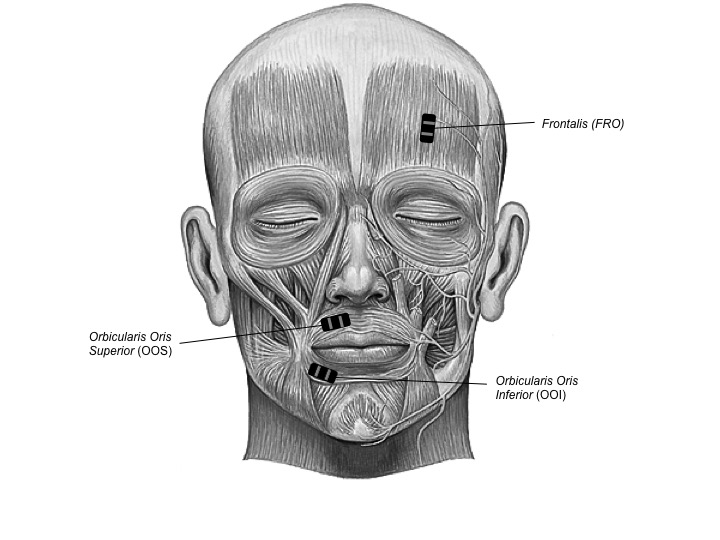
\includegraphics[width=0.75\linewidth]{assets/face_emg} 

}

\caption{Facial muscles of interest. Two speech-related labial muscles: \textit{orbicularis oris superior} (OOS) and \textit{orbicularis oris inferior} (OOI); as well as one non speech-related but sadness-related facial muscle: \textit{frontalis} (FRO).}\label{fig:emgface}
\end{figure}

\subsection{Procedure}\label{procedure}

This study consisted of two parts. The first part was carried out a week
before the EMG experiment and consisted in checking the inclusion
criteria. We checked that participants did not exceed a threshold on a
depressive symptoms scale. This was assessed using the French version of
the \emph{Center for Epidemiologic Studies Depression} scale (CES-D,
Fuhrer \& Rouillon, \protect\hyperlink{ref-fuhrer_version_1989}{1989}),
which evaluates the level of depressive symptom in subclinical
population. We also collected information about any potential speech,
neurologic, neuromuscular or cardiac disorders and about academic
curriculum. Finally, the tendency to ruminate (i.e., trait rumination)
in daily life was evaluated using the French version of the Mini-CERTS
(Cambridge-Exeter Repetitive Thought Scale, Douilliez, Philippot,
Heeren, Watkins, \& Barnard,
\protect\hyperlink{ref-Douilliez2012}{2012}). The second part included
two EMG interdependent experiments related to \emph{Rumination
Induction} and \emph{Rumination Reduction by Muscle Relaxation}.
Specifically, Experiment 1 consisted of acquiring physiological EMG data
during rest and induced rumination and Experiment 2 consisted of
acquiring physiological EMG data after different kinds of relaxation
(see below).

During both Experiment 1 and Experiment 2, momentary rumination was
assessed using four different Visual Analogue Scales (VAS, the first two
being adapted and translated to French from Huffziger, Ebner-Priemer,
Koudela, Reinhard, \& Kuehner,
\protect\hyperlink{ref-Huffziger2012}{2012}) rated from 0 to 100: i)
``At this moment, I am thinking about my feelings'' (referred to as VAS
``\emph{Feelings}''), ii) ``At this moment, I am thinking about my
problems'' (referred to as VAS ``\emph{Problems}''), iii) ``At this
moment, I am brooding about negative things'' (referred to as VAS
``\emph{Brooding}'') and iv) ``At this moment, I am focused on myself''
(referred to as VAS ``\emph{Focused}'').

\subsubsection{Experiment 1: rumination
induction}\label{experiment-1-rumination-induction}

Participants were seated in front of a computer screen in a comfortable
and quiet room. EMG sensors were positioned as explained above (see
Figure \ref{fig:emgface}). Before the rumination induction, each
participant underwent a non-specific relaxation session (i.e., without
targeting specific muscles) in order to minimize inter-individual
initial thymic variability (approximate duration ∼330 s). Immediately
after, participants were instructed to remain silent and not to move for
one minute to carry out EMG ``baseline'' measurements. Then,
participants' initial level of rumination was assessed using the four
VASs.

Subsequently, participants were invited to perform a 15-min I.Q. test,
which was presented on the computer screen facing them. They were
instructed to correctly respond to three types of I.Q. questions
(logical, mathematical and spatial-reasoning questions) in a very short
time (30 s). Most of the questions were very difficult, if not
impossible, to correctly answer in 30 s. We included ten different
questions for each of the three types of I.Q. question: ten logical
questions (e.g., finding the next number of a Fibonacci sequence), ten
mathematical questions (e.g., ``What is the result of the following
calculus: (30/165) − (70/ 66)'') and ten spatial-reasoning questions
(e.g., finding the next figure of a series). Forced-failure tasks have
extensively been employed in the literature to induce a slightly
negative mood, ideal for subsequent rumination induction (e.g., Lemoult
\& Joormann, \protect\hyperlink{ref-Lemoult2014}{2014}; Randenborgh,
Hüffmeier, LeMoult, \& Joormann,
\protect\hyperlink{ref-VanRandenborgh2010}{2010}).

After the I.Q. test, participants were invited to reflect upon the
causes and consequences of their feelings, during five minutes (rumina-
tion induction). This method is based on the induction paradigm
developed by Nolen-Hoeksema \& Morrow
(\protect\hyperlink{ref-nolen-hoeksema_effects_1993}{1993}). The
classical paradigm uses a series of prompts. In order to avoid the
potential confound in muscle activity induced by silent reading, we did
not use the full paradigm. We simply summarised the series of prompts by
one typical induction sentence. During this period, participants were
asked to remain silent and not to move, while EMG recordings were
carried out (i.e., EMG Post-induction measures). EMG signals of
rumination were collected during the last minute of this period.
Finally, participants were instructed to self-report momentary
rumination on the four VASs.

\subsubsection{Experiment 2: rumination reduction by
relaxation}\label{experiment-2-rumination-reduction-by-relaxation}

After Experiment 1, participants were randomly allocated to one of three
groups. In the first group, participants listened to a pre-recorded
relaxation session that was focused on orofacial speech-related muscles
(``\emph{Orofacial Relaxation}'' condition). In the second group,
relaxation was focused on the arm muscles (``\emph{Arm Relaxation}''
condition). In the third group, participants simply listened to a story,
read by the same person, for an equivalent duration (``\emph{Story}''
condition, detailed content of the story can be found in the
\protect\hyperlink{suppCH3}{supplementary materials}, in French). In
summary, the first condition allowed us to evaluate the effects of
targeted speech muscle relaxation on rumination. The second condition
allowed evaluating the effects of a non-orofacial relaxation (i.e.,
speech-unrelated muscles) while the third condition allowed controlling
for effects of attentional distraction during relaxation listening.

The speeches associated with the three conditions, relaxation sessions
and story listening session, were delivered to the participants through
loudspeakers. They were recorded by a professional sophrology therapist
in an anechoic room at GIPSA-lab (Grenoble, France) and were
approximately of the same duration (around 330 s).

After the relaxation/distraction session, participants were asked to
remain silent and not to move during one minute, during which EMG
measurements were collected (EMG Post-relaxation measures). Finally,
participants were instructed to self-report rumination on the four VASs.

\subsection{Data processing and
analysis}\label{data-processing-and-analysis}

\subsubsection{EMG data processing}\label{emg-data-processing}

EMG signal pre-processing was carried out using Labchart 8. The EMG data
were high-pass filtered using a Finite Impulse Response (FIR) filter at
a cut-off of 20 Hz, using the Kaiser window method with \(\beta\) = 6.
Then, output of this first filter was to a low-pass filtered at a
cut-off of 450 Hz (with the same parameters), in order to focus on the
20--450 Hz frequency band, following current recommendations for facial
EMG studies (A. Boxtel,
\protect\hyperlink{ref-boxtel_optimal_2001}{2001}; De Luca,
\protect\hyperlink{ref-de_luca_use_1997}{1997}; De Luca, Donald Gilmore,
Kuznetsov, \& Roy,
\protect\hyperlink{ref-de_luca_filtering_2010}{2010}).

Although we specifically asked participants to remain silent and not to
move during EMG data collection, tiny facial movements (such as biting
one's lips) or vocal productions sometimes occurred. Periods with such
facial movement or vocal production were excluded from the analysis. To
do this, visual inspection of audio, video, and EMG signal was
performed. Specifically, for the EMG signals, we compared two methods of
signal selection. The first one consisted of setting a threshold on the
absolute value of the EMG signal and portions of signals above this
threshold were removed. This threshold was empirically chosen using
visual inspection of a few samples and set to the mean EMG value plus 6
SDs. The second method consisted of manually removing periods of time
that included visually obvious bursts of EMG activity, corresponding to
overt contraction (as in Rapin, Dohen, Polosan, \& Perrier,
\protect\hyperlink{ref-rapin_emg_2013}{2013}). Based on samples from a
few participants, the comparisons between these two methods showed that
the automatic threshold method was somewhat less sensitive to overt
movements. Therefore, the second method was used, as it was more
conservative and less prone to leave data related to irrelevant overt
movements.

After pre-processing, EMG data were exported from Labchart software to
Matlab r2014a (Version 8.3.0.532, www.mathworks.fr). For each EMG
signal, mean values were computed under Matlab, using 200 ms sliding
windows. The average of these mean values were calculated for each
recording session (baseline, after induction and after
relaxation/induction). This provided a score for each muscle of interest
(OOS, OOI, FCR, FRO) in each Session (Baseline, Post-Induction,
Post-Relaxation) for each participant\footnote{Because of constraints
  attributable to the design of our experiment, we were not able to
  perform conventional control measures (e.g., time of the day, food
  consumption, sport activity, smoking habits, etc.). Moreover, in our
  study, periods of signal recording had to be shorter than usual HRV
  analysis time periods (cf.~methodology section). Although recent
  studies suggest that ``ultrashort term'' HRV analysis seems to
  correlate quite well with HRV analysis performed on longer periods of
  time (Brisinda et al.,
  \protect\hyperlink{ref-brisinda_comparison_2013}{2013}; Salahuddin,
  Cho, Jeong, \& Kim, \protect\hyperlink{ref-Salahuddin2007}{2007}), we
  cannot exclude that our measurements might be unreliable. For these
  reasons, we chose not to present HRV results in this report and to
  focus on EMG results as well as subjective reports of rumination.}.

\subsubsection{Statistical analyses}\label{statistical-analyses}

Absolute EMG values are not meaningful as muscle activation is never
null, even in resting conditions, due in part to physiological noise
(Tassinary, Cacioppo, \& Vanman,
\protect\hyperlink{ref-berntson_skeletomotor_2007}{2007}). In addition,
there are inter-individual variations in the amount of EMG activity in
the baseline. To normalise for baseline activity across participants, we
used a differential measure and expressed EMG amplitude as a percentage
of baseline level (Experiment 1) or of post-induction level (Experiment
2).

To model EMG amplitude variations in response to the rumination
induction (Experiment 1) and relaxation (Experiment 2), we used a
bayesian multivariate regression model with the natural logarithm of the
EMG amplitude (expressed in \% of baseline level) as an outcome, in an
intercept-only model (in Experiment 1), and using Condition (Orofacial,
Arm or Story) as a categorical predictor in Experiment 2. We used the
same strategy (two multivariate models) to analyse VAS scores (expressed
in relative changes) along the two experiments.

These analyses were conducted using RStudio (RStudio Team, 2018) and the
\texttt{brms} package (Bürkner, \protect\hyperlink{ref-R-brms}{2018}),
an \texttt{R} implementation of Bayesian multilevel models that employs
the probabilistic programming language \texttt{Stan} (Carpenter et al.,
\protect\hyperlink{ref-carpenter_stan:_2017}{2017}). Stan implements
gradient-based Markov Chain Monte Carlo (MCMC) algorithms (e.g.,
Hamiltonian Monte-Carlo), which allow yielding posterior distributions
that are straightforward to use for interval estimation around all
parameters. Two MCMC simulations (or ``chains'') were run for each
model, including 100,000 iterations, a warmup of 10,000 iterations, and
a thinning interval of 10. Posterior convergence was assessed examining
autocorrelation and trace plots, as well as the Gelman-Rubin statistic.
Fixed effects were estimated via the posterior mean and 95\% highest
density intervals (HDIs), where an HDI interval is the Bayesian analogue
of a classical confidence interval\footnote{While not suffering from the
  misunderstandings associated with frequentist confidence intervals
  (for more details, see for instance Morey et al.,
  \protect\hyperlink{ref-morey_fallacy_2015}{2015}).}.

This strategy allowed us to examine posterior probability distribution
on each parameter of interest (i.e., effects of session and condition on
each response variable). When applicable, we also report evidence ratios
(ERs), computed using the hypothesis function of the \texttt{brms}
package (Bürkner, \protect\hyperlink{ref-R-brms}{2018}). These evidence
ratios are simply the posterior probability under a hypothesis against
its alternative (Bürkner, \protect\hyperlink{ref-R-brms}{2018}). We also
report summary statistics (mean and HDI) of Cohen's d effect sizes,
computed from the posterior samples.

\section{Results}\label{results}

\subsection{Experiment 1: rumination
induction}\label{experiment-1-rumination-induction-1}

The evolution of VAS scores (for the four assessed scales: Feelings,
Problems, Brooding, and Focused) and EMG (for the four muscles: OOS,
OOI, FCR and FRO) activity from baseline to post-induction were
examined.

\subsubsection{Self-reported rumination measures: VAS
scores}\label{self-reported-rumination-measures-vas-scores}

Results for VAS relative changes based on the multivariate models
described earlier are shown in the right panel of Figure
\ref{fig:resultsemgfig1}. Thereafter, \(\alpha\) represents the mean of
the posterior distribution of the intercept. Raw pre- and post-induction
scores are provided in the \protect\hyperlink{suppCH3}{supplementary
materials}.

Mean VAS score on the Feelings scale was slightly lower after induction
(\(\alpha\) = −5.55, 95\% HDI {[}-10.89, −0.24{]}, d = −0.23, 95\% HDI
{[}-0.46, −0.01{]}), while Problems score was slightly higher
(\(\alpha\) = 3.99, 95\% HDI {[}-2.04, 9.83{]}, d = 0.15, 95\% HDI
{[}-0.08, 0.37{]}). We observed a strong increase of the score on the
Brooding scale (\(\alpha\) = 14.45, 95\% HDI {[}8.07, 20.72{]}, d =
0.50, 95\% HDI {[}0.26, 0.74{]}), and a strong decrease on the Focused
scale (\(\alpha\) = −11.63, 95\% HDI {[}-17, −6.07{]}, d = −0.48, 95\%
HDI {[}-0.72, −0.24{]}). As we examined the fit of the intercept-only
model, these estimates represent the posterior mean for each muscle.

In the following, we report the mean (indicated by the Greek symbol
\(\rho\)) and the 95\% HDI of the posterior distribution on the
correlation coefficient (\(\rho\)). Examination of the correlation
matrix estimated by the multivariate model revealed no apparent
correlation neither between Feelings and Problems scales (\(\rho\) =
−0.01, 95\% HDI {[}-0.23, 0.22{]}), nor between Feelings and Brooding
(\(\rho\) = 0.08, 95\% HDI {[}-0.15, 0.30{]}). However, we observed a
strong positive correlation between Problems and Brooding VASs (\(\rho\)
= 0.64, 95\% HDI {[}.49, 0.76{]}), a positive correlation between
Feelings and Focused (\(\rho\) = 0.30, 95\% HDI {[}.08, 0.50{]}), and a
negative correlation between Problems and Focused (\(\rho\) = −0.30,
95\% HDI {[}-0.49, −0.08{]}), as well as between Brooding and Focused
(\(\rho\) = −0.18, 95\% HDI {[}-0.39, 0.05{]}).

\begin{figure}[H]

{\centering 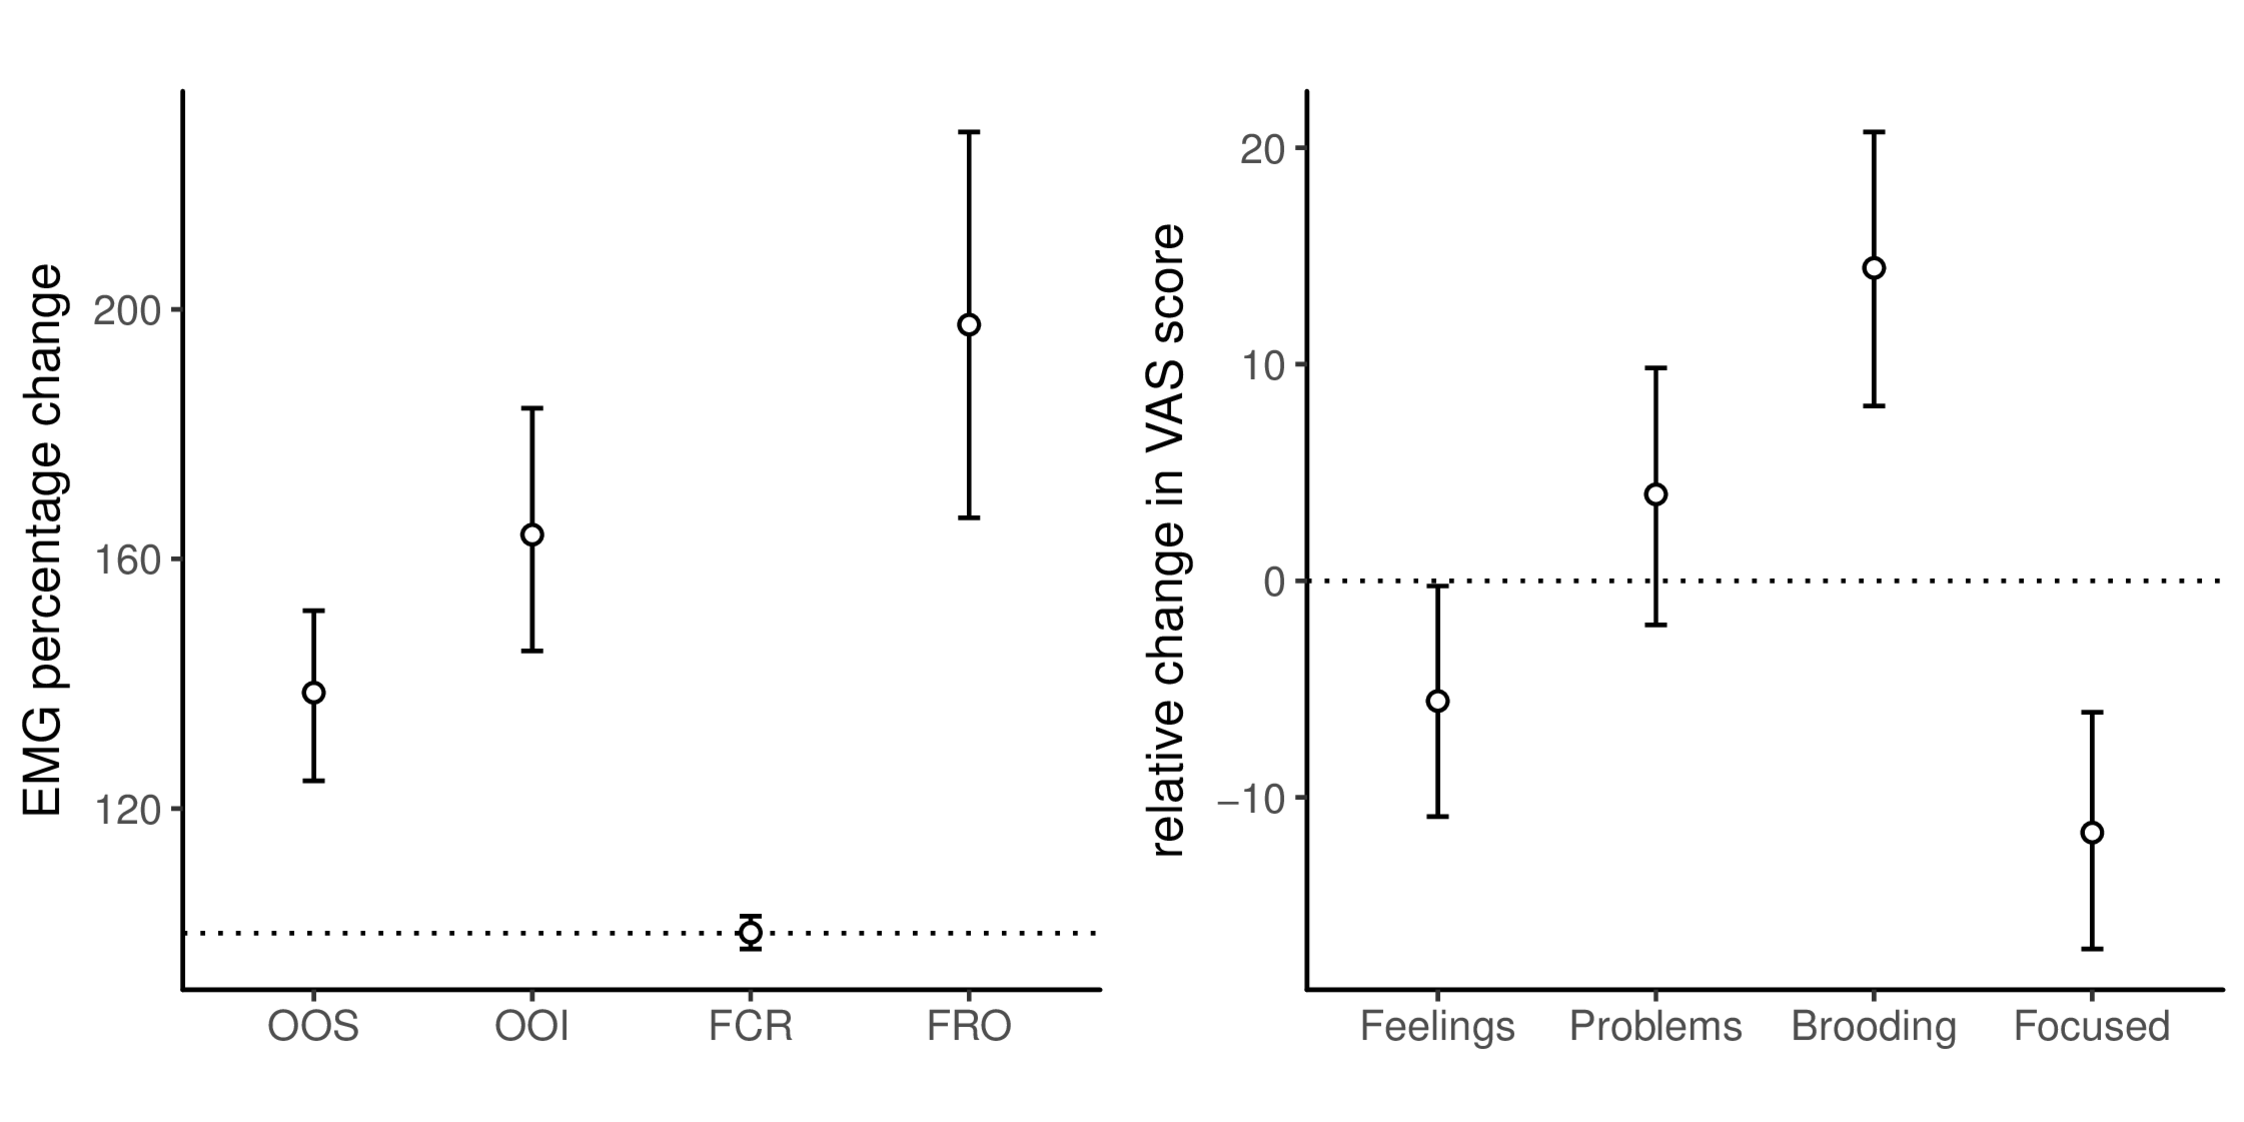
\includegraphics[width=1\linewidth]{assets/emg_fig1} 

}

\caption{Posterior mean (white dots) and 95\% credible intervals for the EMG amplitude (expressed in percentage of baseline level, left panel), and the VAS score (expressed in relative change from baseline, right panel). N = 71 (for each muscle and each VAS). Dashed line represents the null value (i.e., 100\% for the EMG amplitude and 0 for the VAS scores).}\label{fig:resultsemgfig1}
\end{figure}

\subsubsection{EMG}\label{emg}

Results for EMG data based on the multivariate model described earlier
are shown in the left panel of Figure \ref{fig:resultsemgfig1}. Summary
statistics were computed on posterior samples transformed back from log
scale.

Mean EMG amplitude for OOS was higher after induction (\(\alpha\) =
138.57, 95\% HDI {[}124.43, 151.71{]}, d = 0.66, 95\% HDI {[}0.49,
0.84{]}) as well as for OOI (\(\alpha\) = 163.89, 95\% HDI {[}145.24,
184.14{]}, d = 0.77, 95\% HDI {[}0.61, 0.94{]}), and FRO (\(\alpha\) =
197.55, 95\% HDI {[}166.59, 228.42{]}, d = 0.74, 95\% HDI {[}0.59,
0.89{]}). Effects on the FCR were approximately null (\(\alpha\) =
100.10, 95\% HDI {[}97.48, 102.76{]}, d = 0.01, 95\% HDI {[}-0.24,
0.23{]}).

Examination of the correlation matrix estimated by the bayesian
multivariate model revealed a positive correlation between OOS and OOI
EMG amplitudes (\(\rho\) = 0.44, 95\% HDI {[}.24, 0.61{]}), while no
apparent correlations neither between OOS and FCR (\(\rho\) = 0.09, 95\%
HDI {[}-0.14, 0.31{]}), OOS and FRO (\(\rho\) = 0.12, 95\% HDI {[}-0.11,
0.35{]}), OOI and FCR (\(\rho\) = 0.02, 95\% HDI {[}-0.21, 0.25{]}), FRO
and FCR (\(\rho\) = −0.06, 95\% HDI {[}-0.28, 0.17{]}), nor OOI and FRO
(\(\rho\) = 0.07, 95\% HDI {[}-0.16, 0.29{]}). Scatterplots, marginal
posterior distributions and posterior distributions on correlation
coefficients are available in \protect\hyperlink{suppCH3}{supplementary
materials}.

In order to check whether the propensity to ruminate could predict the
effects of the rumination induction on EMG amplitude, we compared the
multivariate model described above, with a similar model but with the
score on the abstract dimension of the Mini-CERTS as an additional
predictor. We compared these models using the widely applicable
information criterion (WAIC; Watanabe, 2010), via the WAIC function of
the \texttt{brms} package (Bürkner,
\protect\hyperlink{ref-R-brms}{2018}). Results showed that the
intercept-only model had a lower WAIC (WAIC = 177.39) than the more
complex model (WAIC = 182.01), indicating that there is no predictive
benefit in adding the Mini-CERTS score as a predictor.

\subsubsection{Correlations between EMG amplitudes and VAS
scores}\label{correlations-between-emg-amplitudes-and-vas-scores}

Correlations between EMG amplitudes and VAS scores were examined using
the \texttt{BayesianFirstAid} package (Bååth,
\protect\hyperlink{ref-R-BayesianFirstAid}{2018}), using 15,000
iterations for each correlation coefficient. Both estimated correlation
coefficients (\(\rho\)s) and 95\% HDIs are reported in Table XX.

\subsection{Experiment 2: rumination reduction by
relaxation}\label{experiment-2-rumination-reduction-by-relaxation-1}

In the second experiment, we aimed at comparing the evolution in EMG
activity and VAS scores from post-induction to post-relaxation in three
different conditions: Orofacial relaxation, Arm relaxation, and
listening to a Story.

\subsubsection{Self-reported rumination measures: VAS
scores}\label{self-reported-rumination-measures-vas-scores-1}

Posterior means and 95\% HDIs of the VAS scores in each condition of
experiment 2 are represented in Figure XX and Table XX.

In order to compare the effects of the two kind of relaxation on the VAS
scores, we then used the \texttt{hypothesis()} function of the
\texttt{brms} package that allows deriving evidence ratios (ER). These
evidence ratios are simply the posterior probability under a hypothesis
(e.g., the hypothesis that the Orofacial relaxation session would be
more effective in reducing self-reported rumination than the Arm
relaxation session) against its alternative (Bürkner,
\protect\hyperlink{ref-R-brms}{2018}).

Since the Problems and the Brooding scales seemed to be sensitive
markers of rumination (as their scores increased after induction in
Experiment 1), our analyses were focused on these two scales.

Concerning the Problems VAS, the decrease observed in the Orofacial
condition was more pronounced than in the Arm condition (Est = −11.06,
SE = 6.35, ER10 = 22.65), and slightly more pro- nounced compared to the
Story condition (Est = −6.05, SE = 6.31, ER10 = 4.98). The observed on
the Brooding VAS score in the Orofacial condition was larger than in the
Arm condition (Est = −9.98, SE = 6.07, ER10 = 18.85), and slightly more
important compared to the Story condition (Est = −5.23, SE = 6.01, ER10
= 4.27).

\begin{figure}[H]

{\centering 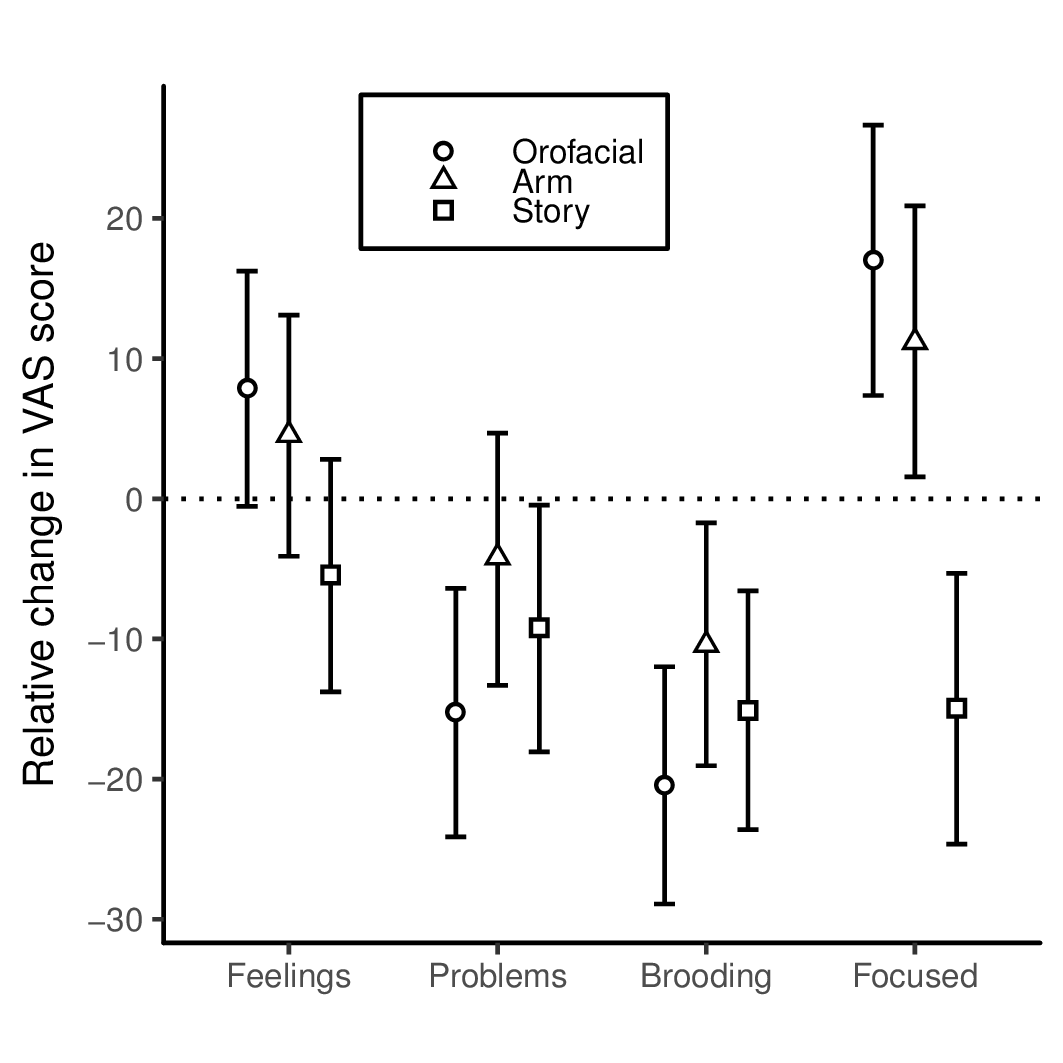
\includegraphics[width=0.75\linewidth]{assets/emg_fig2} 

}

\caption{Posterior mean and 95\% credible intervals for the VAS score (expressed in relative change from post-induction level).}\label{fig:resultsemgfig2}
\end{figure}

\subsubsection{EMG}\label{emg-1}

Posterior means and 95\% HDIs of the EMG amplitude in each condition of
experiment 2 are represented in Figure XX and reported in Table XX. We
used the same strategy as before to compare the effects of the two kinds
of relaxation on the EMG amplitudes.

Concerning the OOS, the observed decrease in the Orofacial condition was
more pronounced than in the Arm condition (Est = −0.34, SE = 0.14, ER10
= 140.73), as well as concerning the OOI (Est = −0.35, SE = 0.19, ER10 =
29.46), while we observed no noticeable differences between the two
kinds of relaxation concerning the EMG amplitude of the FRO (Est =
-0.04, SE = 0.14, ER10 = 1.53).

\begin{figure}[H]

{\centering 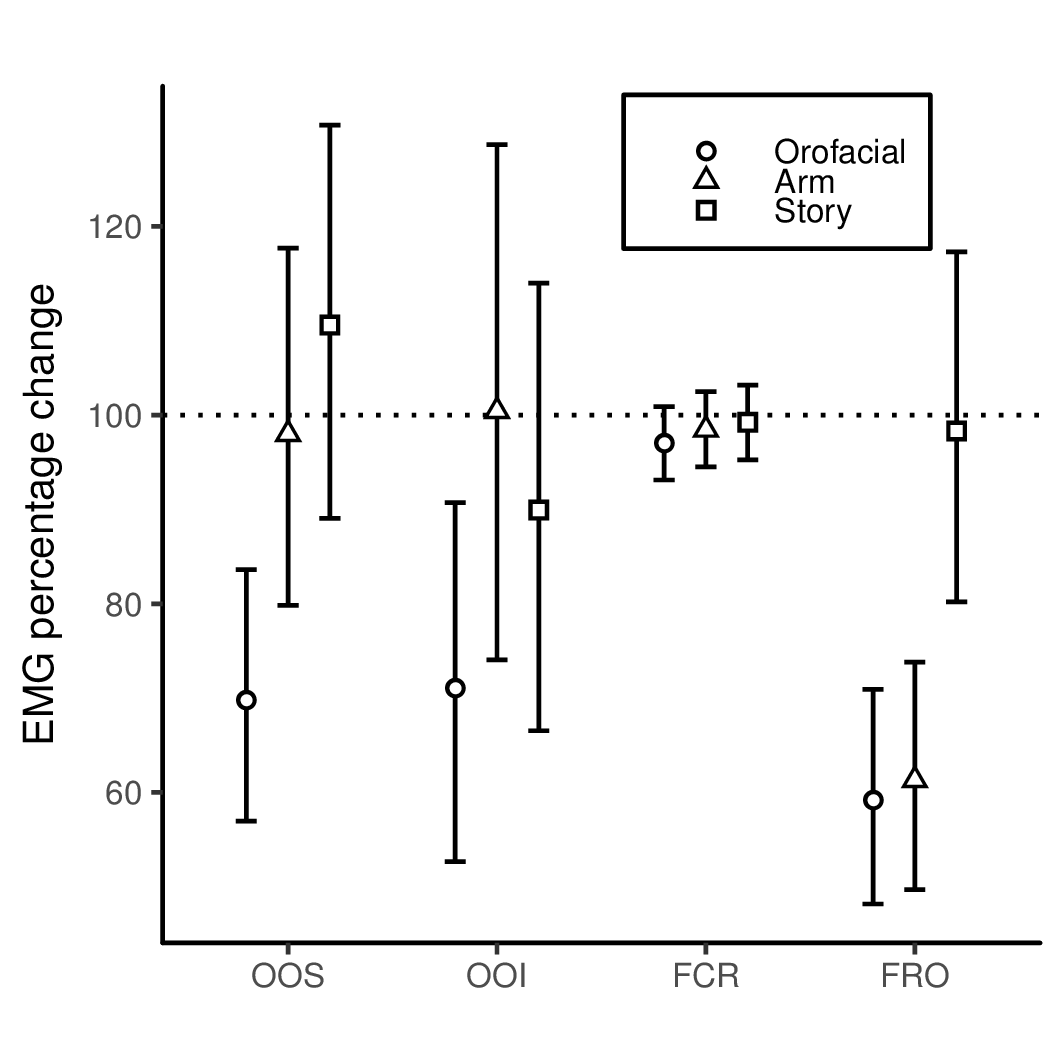
\includegraphics[width=0.75\linewidth]{assets/emg_fig3} 

}

\caption{Posterior mean and 95\% credible intervals for the VAS score (expressed in relative change from post-induction level).}\label{fig:resultsemgfig3}
\end{figure}

\section{Discussion}\label{discussion}

\subsection{Experiment 1}\label{experiment-1}

In the first experiment, we examined electromyographic correlates of
induced rumination in healthy individuals. According to the \emph{Motor
Simulation view}, we predicted an increase in the activity of all facial
muscles after the rumination induction, associated with an increase in
self-reported rumination. Alternatively, the \emph{Abstraction view}
predicted an increase in self-reported rumination associated with an
increase in forehead activity with no changes in either lip or forearm
activity.

To test the predictions of these two theoretical views, we compared EMG
measures and VAS scores after induction to their values before
induction. EMG activity was examined in four muscles: OOS and OOI, two
muscles involved in speech production, FRO, a facial negative-
affect-related but not speech-related muscle, and FCR, a non-facial
control muscle on the non-dominant forearm.

As predicted by the \emph{Motor Simulation view}, we observed an
increase in the activity of the two speech-related muscles (OOS \& OOI)
as well as in the negative-affect-related muscle (FRO) and no change in
FCR activity. The increase in facial EMG together with the increase in
the subjective reports of rumination suggests that facial EMG increase
is a correlate of verbal rumination. As supported by several studies
results, the forehead muscle activity has been associated with
unpleasant emotions (Jäncke et al.,
\protect\hyperlink{ref-Jancke1996}{1996}) or anxiety (A. Conrad \& Roth,
\protect\hyperlink{ref-conrad_muscle_2007}{2007}). The increase in FRO
activity observed here is consistent with the increase in negative
emotions induced by our negatively valenced induction procedure.
\emph{Orbicularis oris} lip muscles are associated with speech
production. The increase in lip activity observed here suggests that the
speech motor system was involved during the ruminative phase. The fact
that the FCR remained stable after rumination induction suggests that
the observed facial activity increase was not due to general body
tension induced by a negative mental state. These facial EMG results
therefore support the hypothesis that rumination is an instance of
articulatory-specified inner speech.

After the rumination induction, a larger increase in OOI activity was
observed compared to the increase in OOS activity. This finding is
consistent with previous findings of higher EMG amplitude in the lower
lip during speech and inner speech (e.g., S. M. Barlow \& Netsell,
\protect\hyperlink{ref-barlow_differential_1986}{1986}; Regalo et al.,
\protect\hyperlink{ref-regalo_electromyographic_2005}{2005}; Sokolov,
\protect\hyperlink{ref-sokolov_inner_1972}{1972}) or auditory verbal
hallucinations (Rapin et al.,
\protect\hyperlink{ref-rapin_emg_2013}{2013}). Rapin et al.
(\protect\hyperlink{ref-rapin_emg_2013}{2013}) have explained the
difference between the activities of the two lip muscles by muscle
anatomy. The proximity of the OOI muscle with other speech muscles (such
as the depressor angular muscle or the mentalis) could increase the
surface EMG signal captured on the lower lip (OOI), as compared to the
upper lip (OOS) during speech. An even larger increase in FRO activity
was observed compared to the increase in lip muscle activity. As EMG
amplitude is known to vary with muscle length (Babault et al.,
\protect\hyperlink{ref-babault_effect_2003}{2003}), the greater increase
in frontalis activity could be explained by its anatomical properties.

However, although a functional distinction can be drawn between the
forehead and the lip muscles, one should acknowledge the fact that these
two sets of muscles can be commonly activated during some behaviours.
For instance, A. van Boxtel \& Jessurun
(\protect\hyperlink{ref-van_boxtel_amplitude_1993}{1993}) have shown
that orbicularis oris inferior and frontalis were both activated during
a two-choice serial reaction task in which nonverbal auditory or visual
signals were presented. Moreover, there was a gradual increase in EMG
activity in these muscles during the task, either when the task was
prolonged or when the task was made more difficult. They interpreted
this increase in EMG activity as associated with a growing compensatory
effort to keep performance at an adequate level. An alternative
interpretation is that the increase in task difficulty was dealt with by
inner verbalization. Covertly rehearsing the instructions or covertly
qualifying the stimuli might have helped the participants to perform
adequately. Therefore, the increase in orbicularis oris activity might
have been related to an increase in covert verbalization, whereas the
increase in frontalis activity might have been related to increased
anxiety or tension. The fact that the EMG increase was muscle specific,
and that some facial muscles (\emph{orbicularis oculi},
\emph{zygomaticus major}, \emph{temporalis}) did not show an increase in
activity unless the task became too difficult, supports this
interpretation. It cannot be ruled out, however, that orbicularis oris
activity may in some cases be related to mental effort without mental
verbalisation. Nevertheless, although the I.Q. test itself was designed
to induce mental effort, no cognitively demanding task was asked to the
participant during the period of EMG recording (i.e., approximately four
minutes after the end of the test). Although we cannot absolutely
exclude that rumination in itself could require cognitive effort, it
seems unlikely that mental effort was the main factor of variation.

Scores on the VAS need to be discussed in further detail. We examined
which VAS scales were most suitable to capture changes in state
rumination to allow focused analyses. Due to the ``pre-baseline''
relaxation session, during which participants were asked to concentrate
on their body and breathing cycles, participants reported a high level
of attentional self-focus at baseline (``Feelings'' and ``Focused''
VAS). Because of the high level of self-focused attention at baseline,
it is likely that the scores on the ``Feelings'' and ``Focused'' VAS did
not show the expected increase after rumination induction (ceiling
effect). The scores on the scales ``Problems'' and ``Brooding'', which
are more representative of maladaptive rumination, did increase after
our rumination induction paradigm, however. Interestingly, the
``Brooding'' VAS corresponded to a larger increase and seemed to be more
sensitive to rumination induction than the ``Problems'' VAS. Given this
greater sensibility and the strong positive correlation between the
``Brooding'' and the ``Problems'' VAS, it thus make sense to consider
the ``Brooding'' VAS as a better estimate of ruminative state, at least
within our paradigm. We will therefore only use this scale to assess
rumination in the following.

The fact that we did not observe any association between the propensity
to ruminate (as measured by the Mini-CERTS questionnaire) and the
effects of the induction is consistent with the results of Rood,
Roelofs, Bögels, \& Arntz (\protect\hyperlink{ref-Rood2012}{2012}) who
found that the level of trait rumination did not moderate the effects of
a rumination induction.

\subsection{Experiment 2}\label{experiment-2}

In the second experiment, we studied the effects of two muscle-specific
relaxation sessions: Orofacial relaxation and Arm relaxation. We
compared their effects to a third control condition (Story), which did
not involve the deliberate relaxation of any specific muscle. Our
predictions were that a decrease in facial EMG activity should be
observed in each condition. If the \emph{Motor Simulation view} is
correct, we expected a larger decrease in the activity of all facial
muscles in the ``Orofacial relaxation'' condition than in the ``Arm
relaxation'' condition, associated with a larger decrease in
self-reported rumination. Additionally, we expected a more pronounced
decrease in the two relaxation conditions (orofacial and arm relaxation
conditions) than in the control (``Story'') condition. We also expected
no difference between relaxation conditions regarding the change in the
forearm muscle activity.

The data indicated a decrease in self-reported rumination (``Brooding''
VAS) in each condition. The ``Orofacial'' relaxation condi- tion
elicited a slightly larger decrease than the ``Arm relaxation'' or the
``Story'' condition. However, there was extensive individual variation
in response to these conditions. As concerns EMG results, we observed a
decrease in OOS and OOI activities in all three conditions but this
decrease was more pronounced in the orofacial condition than in the
other two conditions. The frontalis activity did not show the same
pattern. A similar FRO activity decrease was observed in both the
orofacial and the non-orofacial relaxation conditions. Therefore, in
Experiment 2, the lip muscles and the forehead muscle follow
differential evolutions. A dissociation was observed: whereas both
orofacial and arm relaxations resulted in a decrease in forehead
activity, only orofacial relaxation was successful at reducing lip
activity.

Considering both VAS results and the dissociation in EMG patterns,
several interpretations are possible. The first interpretation is that
verbal production associated with rumination was more reduced by
orofacial muscular relaxation than by non-orofacial relaxation. This
interpretation is consistent with the fact that the ``Brooding'' VAS was
slightly more decreased in this condition compared to the other two. The
larger decrease in OOS and OOI amplitude after orofacial relaxa- tion
would thus reflect this reduction in verbal production, as hypothesised
by the \emph{Motor Simulation view}. The fact that FRO activity
displayed a similar decrease in both orofacial and non-orofacial
relaxation conditions could suggest that any means of body relaxation
(be it orofacial or not) is appropriate to reduce negative affect and
can therefore reduce forehead contraction. This suggests that the FRO
activity increase presumably reflected negative affect and tension (such
as observed in EMG studies on generalised anxiety disorder patients, see
A. Conrad \& Roth, \protect\hyperlink{ref-conrad_muscle_2007}{2007}, for
a review).

Alternatively, one could also argue that the larger decrease in lip
muscle activity after orofacial relaxation finds a more trivial explana-
tion in that it seems obvious to expect that orofacial relaxation will
be more efficient to reduce lip muscle contraction than non-orofacial
relaxation. Thus, the different impacts of the two relaxation sessions
on the lip muscles would not be related to reduced rumination per se but
simply to a more anatomically targeted relaxation. However, several
observations argue against such an interpretation. The larger decrease
in the ``Brooding'' VAS in the orofacial relaxation condition compared
with the other conditions suggests that the reduction in lip muscle
activity is indeed related to the reduction in rumination. Moreover, an
interpretation solely based on anatomical links does not explain why FRO
activity displayed the same amount of reduction in both relaxation
sessions. If reduction in muscle activity was merely related to the
effect of facial muscle relaxation, then the decrease in FRO activity
should have also been higher in the orofacial relaxation condition than
in the other relaxation condition, which was not the case. Therefore the
dissociation between forehead and lip patterns of activity, together
with the differential effects of the two types of relaxation on
subjective rumination reports strongly suggest that different processes
underlie the activity of these two sets of muscles. We therefore
consider that the first interpretation is more plausible: frontalis
activity seems related to overall facial tension due to negative affect
whereas lip activity seems to be related to the specific involvement of
the speech musculature in rumination. These results thus seem to confirm
the interpretation of decreased OOS and OOI activities in the orofacial
relaxation condition as markers of rumination reduction.

Interestingly, we observed no changes of forearm EMG activity in any of
the three conditions of Experiment 2. The fact that the relaxation
session focused on the forearm was not associated with a decrease in FCR
activity has a simple explanation: FCR activity had not increased after
rumination induction and had remained at floor level. The forearm was
thus already relaxed and the Arm relaxation session did not modify FCR
activity. Another interesting conclusion related to this absence of
modification of forearm activity is that relaxation does not spuriously
decrease muscle activity below its resting level. One possible
interpretation of the increase in lip EMG after rumination induction
could have been that baseline relaxation artificially decreased baseline
activity under its resting level. The facts that forearm activity did
not decrease after arm-focused relaxation contradicts this
interpretation.

Finally, the ``Story'' condition was also associated with a decrease in
OOI and FRO activities. This could mean that listening to a story
reduced rumination to the same extent as relaxation did. However, the
discrepancy observed in ``Focused'' VAS between the two relaxation
conditions on the one hand and the control condition on the other hand,
suggests that the EMG decrease observed in the ``Story'' condition might
be attributable to a different cause than that observed in the two
relaxation conditions. Listening to a story could help reducing
rumination by shifting attention away from ruminative thoughts.
Relaxation sessions could help reducing rumination by shifting attention
to the body in a beneficial way.

\subsection{General discussion}\label{general-discussion}

We set out two experiments to examine whether rumination involves motor
simulation or is better described as linguistically abstract and
articulatory impoverished. We used labial, facial, and arm EMG measures
to assess potential articulatory correlates of rumination. The patterns
of results of our study seem to be in favour of the motor nature of
verbal rumination. In Experiment 1, rumination induction was associated
with a higher score on the scale ``I am brooding about negative things''
which is representative of abstract-analytical rumination, considered as
verbal rumination. This maladap- tive rumination state was associated
with an increase in the activity of two speech-related muscles, without
modification of the arm muscle activity, which indicates that rumination
involves activity in speech articulatory muscles, specifically. The
concurrent increase in forehead muscle activity could be explained by an
increase in negative emotions induced by our negatively valenced
induction procedure. The results of Experiment 1 therefore show the
involvement of the speech muscula- ture during rumination. This is in
line with the \emph{Motor simulation view}, according to which inner
speech is fully specified at the articulatory level, not just the
lexical level.

In Experiment 2, guided relaxation resulted in a decrease in speech
muscle activity. In the lip muscles, the activity decrease was stronger
after orofacial relaxation than after arm-focused relaxation. In the
forehead muscle, however the effect was the same for both types of
relaxation. This decrease in speech muscle activity was associated with
a decrease in self-reports of rumination and was most pronounced after
orofacial relaxation. These findings suggest that a reduction in speech
muscle activity could hinder articulatory simulation and thus limit
inner speech production and therefore reduce rumination. This
interpretation is consistent with the \emph{Motor Simulation view} of
inner speech. Brooding-type rumination was also diminished after the
arm-focused relaxation as well as after listening to a story, although
less than in the orofacial relaxation. This suggests that general
relaxation or distraction are also likely to reduce negative rumination.
To summarize, experiments 1 and 2 are consistent with the \emph{Motor
Simulation view} of inner speech, according to which speech muscle
activity is inherent to inner speech production. Experiment 1 shows the
involvement of the lip musculature during brooding-type rumination.
Experiment 2 suggests that brooding-type rumination could be reduced by
blocking or relaxing speech muscles.

These data support the utility of labial EMG as a tool to objectively
assess inner speech in a variety of normal and pathological forms. We
suggest that this method could be used as a complement to self-report
measures, in order to overcome limitation of these measures.

Our results should be interpreted with some limitations in mind. First,
our sample consisted exclusively of women. Although this methodological
choice makes sense considering the more frequent occurrence of
rumination in women, further studies should be conducted to ascertain
that our results may generalize to men. Second, in Experiment 1, no
between-subject control condition was used to compare with the group of
participants who underwent rumination induction. Thus, we cannot rule
out that other processes occurred between baseline and rumination
induction, influencing responding. Thirdly, substantial inter-individual
differences were observed concerning the size of the effect of
rumination induction on facial EMG activity. The results of Jäncke
(Jäncke, \protect\hyperlink{ref-Jancke1996a}{1996}; Jäncke et al.,
\protect\hyperlink{ref-Jancke1996}{1996}) can shed light on this last
result. Jäncke used a similar procedure (i.e., negative mood induction
using a false I.Q. test and facial EMG measurements to assess emotions),
except that the experimenter was not in the room while participants
performed the test and acknowledged their results. The experimenter then
came back to the room and analysed participants' behaviours. Jäncke
observed an increase in facial muscular activity (assessed when
participants were reading their results) only in partici- pants who were
prone to express their distress when the experimenter came back, while
more introverted participants did not show any increased facial activity
when reading their results. Jäncke interpreted these results in the
framework of an ecological theory of facial expression, suggesting that
facial expressions would not only be guided by underlying emotions, but
also by their communicative properties. Considering these results, it
seems likely that the proneness of participants to communicate their
emotions could have mediated effects of the induction on their facial
EMG activity. This could partially explain the observed inter-individual
variability in facial EMG activity associated with rumination. Moreover,
even though rumination is a predominantly verbal process, one cannot
exclude that some of our participants experienced rumination in another
modality (e.g., imagery-based rumination), which would explain their
lower than average lip activity.

Thus, a logical next step is to examine qualitative factors that mediate
the link between rumination and facial muscular activity. These factors
(among others) could be proneness to communicate emotion or proneness to
verbalize affects. Additionally, recent studies suggest a link between
verbal aptitudes and propensity to ruminate. Uttl, Morin, \& Hamper
(\protect\hyperlink{ref-Uttl2011}{2011}) have observed a weak but
consistent correlation between the tendency to ruminate and scores on a
verbal intelligence test. Penney, Miedema, \& Mazmanian
(\protect\hyperlink{ref-Penney2015}{2015}) have observed that verbal
intelligence constitutes a unique predictor of rumination severity in
chronic anxious patients. To our knowledge, the link between verbal
intelligence and induced rumination has never been studied. It would be
interesting to examine whether the effects of a rumination induction
could be mediated by verbal intelligence, and to what extent this could
influence related facial EMG activity.

In conclusion, this study provides new evidence for the facial
embodiment of rumination, considered as a particular instance of inner
speech. Even if more data are needed to confirm these preliminary
conclusions, our results seem to support the \emph{Motor Simulation
view} of inner speech production, manifested as verbal rumination. In
addition, facial EMG activity provides a useful means to objectively
quantify the presence of verbal rumination.

\section{Acknowledgements}\label{acknowledgements-1}

This project was funded by the ANR project INNERSPEECH. The first author
of the manuscript is funded by a fellowship from Université Grenoble
Alpes and a grant from the Pôle Grenoble Cognition. We thank Nathalie
Vallet for recording the relaxation and distraction sessions. We thank
our colleagues from GIPSA-lab: Marion Dohen for her help in the
recording of the audio stimuli in the anechoic room at GIPSA-lab, as
well as Christophe Savariaux and Coriandre Vilain for their advice in
the audio setup associated with the EMG measures. We are also grateful
to Rafael Laboissière and Adeline Leclercq Samson for their advice
concerning data analysis. We sincerely thank two anonymous reviewers for
their critical reading of our manuscript and their many insightful
comments and suggestions. Access to the facility of the MSH-Alpes SCREEN
platform for conducting research is gratefully acknowledged.

\hypertarget{suppCH3}{\section{Supplementary data}\label{suppCH3}}

Supplementary data associated with this article can be found at
\url{https://osf.io/882te/}.

\newpage

\begin{vplace}[1]

\begin{summary}{Summary of Chapter\getcurrentref{chapter}}

In this first experiment we... Rumination is predominantly experienced in the form of repetitive verbal thoughts. Verbal rumination is a particular case of inner speech. According to the Motor Simulation view, inner speech is a kind of motor action, recruiting the speech motor system. In this framework, we predicted an increase in speech muscle activity during rumination as compared to rest. We also predicted increased forehead activity, associated with anxiety during rumination. We measured electromyographic activity over the orbicularis oris superior and inferior, frontalis and flexor carpi radialis muscles. Results showed increased lip and forehead activity after rumination induction compared to an initial relaxed state, together with increased self-reported levels of rumination. Moreover, our data suggest that orofacial relaxation is more effective in reducing rumination than non-orofacial relaxation. Altogether, these results support the hypothesis that verbal rumination involves the speech motor system, and provide a promising psychophysiological index to assess the presence of verbal rumination.\\

Blah blah...

\end{summary}

\end{vplace}

\chapter{Dissociating facial electromyographic correlates of visual and
verbal induced
rumination}\label{dissociating-facial-electromyographic-correlates-of-visual-and-verbal-induced-rumination}

Summary of the research\ldots{}\footnote{This experimental chapter is a
  submitted manuscript reformatted for the need of this thesis.
  Pre-registered protocol, preprint, data, as well as reproducible code
  and figures are available at: \url{https://osf.io/c9pag/}.}

\begin{summary}{Summary of Chapter\getcurrentref{chapter}}

Blah blah ...

\end{summary}

\chapter{Muscle-specific electromyographic correlates of inner speech
production}\label{muscle-specific-electromyographic-correlates-of-inner-speech-production}

Summary of the research\ldots{}\footnote{This experimental chapter is a
  submitted manuscript reformatted for the need of this thesis.
  Pre-registered protocol, preprint, data, as well as reproducible code
  and figures are available at: \url{https://osf.io/czer4/}.}

\begin{summary}{Summary of Chapter\getcurrentref{chapter}}

Blah blah ...

\end{summary}

\chapter{Articulatory suppression effects on induced
rumination}\label{articulatory-suppression-effects-on-induced-rumination}

Summary of the research\ldots{}\footnote{This experimental chapter is a
  submited manuscript reformatted for the need of this thesis.
  Pre-registered protocol, preprint, data, as well as reproducible code
  and figures are available at: \url{https://osf.io/3bh67/}.}

\begin{summary}{Summary of Chapter\getcurrentref{chapter}}

Blah blah ...

\end{summary}

\chapter{Refining the involvement of the speech motor system during
rumination: a dual-task
investigation}\label{refining-the-involvement-of-the-speech-motor-system-during-rumination-a-dual-task-investigation}

Summary of the research\ldots{}\footnote{This experimental chapter is a
  submitted manuscript reformatted for the need of this thesis.
  Pre-registered protocol, preprint, data, as well as reproducible code
  and figures are available at: \url{https://osf.io/8ab2d/}.}

\begin{summary}{Summary of Chapter\getcurrentref{chapter}}

Blah blah ...

\end{summary}

\part{Discussion and
conclusions}\label{part-discussion-and-conclusions}

\chapter{Discussion and perspectives}\label{discussion-and-perspectives}

\section{Summary of the results}\label{summary-of-the-results}

\ldots{}

\section{Benchmarks for theories of inner
speech}\label{benchmarks-for-theories-of-inner-speech}

A revised verson of MacKay
(\protect\hyperlink{ref-mackay_constraints_1992}{1992})
constraints\ldots{}

\section{Limitations and ways
forward}\label{limitations-and-ways-forward}

\ldots{}

\section{Conclusions}\label{conclusions}

\ldots{}

\chapter*{References}\label{references}
\addcontentsline{toc}{chapter}{References}

\noindent
\setlength{\parindent}{-0.20in} \setlength{\leftskip}{0.20in}
\setlength{\parskip}{8pt}

\hypertarget{refs}{}
\hypertarget{ref-abramson_what_1997}{}
Abramson, M., \& Goldinger, S. D. (1997). What the reader's eye tells
the mind's ear: Silent reading activates inner speech. \emph{Perception
\& Psychophysics}, \emph{59}(7), 1059--1068.
\url{https://doi.org/10.3758/BF03205520}

\hypertarget{ref-agnati_possible_2012}{}
Agnati, L. F., Barlow, P., Ghidoni, R., Borroto-Escuela, D. O.,
Guidolin, D., \& Fuxe, K. (2012). Possible genetic and epigenetic links
between human inner speech, schizophrenia and altruism. \emph{Brain
Research}, \emph{1476}, 38--57.
\url{https://doi.org/10.1016/j.brainres.2012.02.074}

\hypertarget{ref-alderson-day_inner_2015}{}
Alderson-Day, B., \& Fernyhough, C. (2015). Inner speech: Development,
cognitive functions, phenomenology, and neurobiology.
\emph{Psychological Bulletin}, \emph{141}(5), 931--965.
\url{https://doi.org/10.1037/bul0000021}

\hypertarget{ref-anderson_speech_1982}{}
Anderson, R. E. (1982). Speech imagery is not always faster than visual
imagery. \emph{Memory \& Cognition}, \emph{10}(4), 371--380.
\url{https://doi.org/10.3758/BF03202429}

\hypertarget{ref-babault_effect_2003}{}
Babault, N., Pousson, M., Michaut, A., \& Van Hoecke, J. (2003). Effect
of quadriceps femoris muscle length on neural activation during
isometric and concentric contractions. \emph{Journal of Applied
Physiology}, \emph{94}(3), 983--990.
\url{https://doi.org/10.1152/japplphysiol.00717.2002}

\hypertarget{ref-baddeley_working_1986}{}
Baddeley, A. (1986). \emph{Working memory}. New York, NY, US: Clarendon
Press/Oxford University Press.

\hypertarget{ref-baddeley_phonological_1985}{}
Baddeley, A. D., \& Wilson, B. (1985). Phonological coding and
short-term memory in patients without speech. \emph{Journal of Memory
and Language}, \emph{24}(4), 490--502.
\url{https://doi.org/10.1016/0749-596X(85)90041-5}

\hypertarget{ref-bakan_test_1966}{}
Bakan, D. (1966). The test of significance in psychological research.
\emph{Psychological Bulletin}, \emph{66}(6), 423--437.
\url{https://doi.org/10.1037/h0020412}

\hypertarget{ref-barlow_differential_1986}{}
Barlow, S. M., \& Netsell, R. (1986). Differential Fine Force Control of
the Upper and Lower Lips. \emph{Journal of Speech, Language, and Hearing
Research}, \emph{29}(2), 163--169.
\url{https://doi.org/10.1044/jshr.2902.163}

\hypertarget{ref-Barsalou2008}{}
Barsalou, L. W. (2008). Grounded cognition. \emph{Annual Review of
Psychology}, \emph{59}, 617--645.
\url{https://doi.org/10.1146/annurev.psych.59.103006.093639}

\hypertarget{ref-basho_effects_2007}{}
Basho, S., Palmer, E. D., Rubio, M. A., Wulfeck, B., \& Müller, R.-A.
(2007). Effects of generation mode in fMRI adaptations of semantic
fluency: Paced production and overt speech. \emph{Neuropsychologia},
\emph{45}(8), 1697--1706.
\url{https://doi.org/10.1016/j.neuropsychologia.2007.01.007}

\hypertarget{ref-R-BayesianFirstAid}{}
Bååth, R. (2018). \emph{BayesianFirstAid: Bayesian replacements for the
most commonly used statistical tests in r.} Retrieved from
\url{http://www.sumsar.net}

\hypertarget{ref-binet_psychologie_1886}{}
Binet, A. (1886). \emph{La psychologie du raisonnement. Recherches
expérimentales par l'hypnotisme}. Alcan, Paris.

\hypertarget{ref-bonnet_mental_1997}{}
Bonnet, M., Decety, J., Jeannerod, M., \& Requin, J. (1997). Mental
simulation of an action modulates the excitability of spinal reflex
pathways in man. \emph{Cognitive Brain Research}, \emph{5}(3), 221--228.
\url{https://doi.org/10.1016/S0926-6410(96)00072-9}

\hypertarget{ref-boxtel_optimal_2001}{}
Boxtel, A. (2001). Optimal signal bandwidth for the recording of surface
EMG activity of facial, jaw, oral, and neck muscles.
\emph{Psychophysiology}, \emph{38}(1), 22--34.
\url{https://doi.org/10.1111/1469-8986.3810022}

\hypertarget{ref-van_boxtel_amplitude_1993}{}
Boxtel, A. van, \& Jessurun, M. (1993). Amplitude and bilateral
coherency of facial and jaw-elevator EMG activity as an index of effort
during a two-choice serial reaction task. \emph{Psychophysiology},
\emph{30}(6), 589--604.
\url{https://doi.org/10.1111/j.1469-8986.1993.tb02085.x}

\hypertarget{ref-boyd_reflective_1983}{}
Boyd, E. M., \& Fales, A. W. (1983). Reflective Learning: Key to
Learning from Experience. \emph{Journal of Humanistic Psychology},
\emph{23}(2), 99--117. \url{https://doi.org/10.1177/0022167883232011}

\hypertarget{ref-rubin_what_1986}{}
Brewer, W. F. (1986). What is autobiographical memory? In D. C. Rubin
(Ed.), \emph{Autobiographical Memory} (pp. 25--49). Cambridge: Cambridge
University Press. \url{https://doi.org/10.1017/CBO9780511558313.006}

\hypertarget{ref-brisinda_comparison_2013}{}
Brisinda, D., Venuti, A., Sorbo, A., Cataldi, C., Iantorno, E., \&
Fenici, R. (2013). Comparison between standard short-term, very-short
and ultra-short-term heart rate variability analysis in healthy subjects
during exercise testing. \emph{European Heart Journal},
\emph{34}(suppl\_1).
\url{https://doi.org/10.1093/eurheartj/eht309.P3384}

\hypertarget{ref-burnham_model_2002}{}
Burnham, K. P., \& Anderson, D. R. (2002). \emph{Model selection and
multimodel inference: A practical information-theoretic approach} (2nd
ed). New York: Springer.

\hypertarget{ref-burnham_multimodel_2004}{}
Burnham, K. P., \& Anderson, D. R. (2004). Multimodel Inference:
Understanding AIC and BIC in Model Selection. \emph{Sociological Methods
\& Research}, \emph{33}(2), 261--304.
\url{https://doi.org/10.1177/0049124104268644}

\hypertarget{ref-R-brms}{}
Bürkner, P.-C. (2018). \emph{Brms: Bayesian regression models using
'stan'}. Retrieved from \url{https://CRAN.R-project.org/package=brms}

\hypertarget{ref-carpenter_stan:_2017}{}
Carpenter, B., Gelman, A., Hoffman, M., Lee, D., Goodrich, B.,
Betancourt, M., \ldots{} Riddell, A. (2017). Stan: A Probabilistic
Programming Language. \emph{Journal of Statistical Software, Articles},
\emph{76}(1), 1--32. \url{https://doi.org/10.18637/jss.v076.i01}

\hypertarget{ref-cefidekhanie_interaction_2014}{}
Cefidekhanie, A. H., Savariaux, C., Sato, M., \& Schwartz, J.-l. (2014).
Interaction between articulatory gestures and inner speech in a counting
task. \emph{Journal of the Acoustical Society of America},
\emph{136}(4), 1869--1879. \url{https://doi.org/10.1121/1.4893910}

\hypertarget{ref-christoff_mind-wandering_2016}{}
Christoff, K., Irving, Z. C., Fox, K. C. R., Spreng, R. N., \&
Andrews-Hanna, J. R. (2016). Mind-wandering as spontaneous thought: A
dynamic framework. \emph{Nature Reviews Neuroscience}, \emph{17}(11),
718--731. \url{https://doi.org/10.1038/nrn.2016.113}

\hypertarget{ref-cohen_motor_1986}{}
Cohen, B. H. (1986). The motor theory of voluntary thinking. In R. J.
Davidson, G. E. Schartz, \& D. Shapiro (Eds.), \emph{Consciousness and
self-regulation}. Springer, Boston, MA.

\hypertarget{ref-coltheart_phonological_1999}{}
Coltheart, V. (1999). Phonological codes in reading comprehension,
short-term memory, and memory for rapid visual sequences. In
\emph{Fleeting memories: Cognition of brief visual stimuli} (pp.
181--223). Cambridge, MA, US: The MIT Press.

\hypertarget{ref-conrad_muscle_2007}{}
Conrad, A., \& Roth, W. T. (2007). Muscle relaxation therapy for anxiety
disorders: It works but how? \emph{Journal of Anxiety Disorders},
\emph{21}(3), 243--264.
\url{https://doi.org/10.1016/j.janxdis.2006.08.001}

\hypertarget{ref-conrad_speech_1979}{}
Conrad, B., \& Schönle, P. (1979). Speech and respiration. \emph{Archiv
Für Psychiatrie Und Nervenkrankheiten}, \emph{226}(4), 251--268.
\url{https://doi.org/10.1007/BF00342238}

\hypertarget{ref-conway_autobiographical_1990}{}
Conway, M. A. (1990). \emph{Autobiographical memory: An introduction.}
Open University Press.

\hypertarget{ref-corley_error_2011}{}
Corley, M., Brocklehurst, P. H., \& Moat, H. S. (2011). Error biases in
inner and overt speech: Evidence from tongue twisters. \emph{Journal of
Experimental Psychology: Learning, Memory, and Cognition}, \emph{37}(1),
162--175. \url{https://doi.org/10.1037/a0021321}

\hypertarget{ref-Cumming2012}{}
Cumming, G. (2012). \emph{Understanding the new statistics: Effect
sizes, confidence intervals, and meta-analysis.} (New York:).

\hypertarget{ref-cumming_new_2014}{}
Cumming, G. (2014). The New Statistics: Why and How. \emph{Psychological
Science}, \emph{25}(1), 7--29.
\url{https://doi.org/10.1177/0956797613504966}

\hypertarget{ref-de_luca_use_1997}{}
De Luca, C. J. (1997). The Use of Surface Electromyography in
Biomechanics. \emph{Journal of Applied Biomechanics}, \emph{13}(2),
135--163. \url{https://doi.org/10.1123/jab.13.2.135}

\hypertarget{ref-de_luca_filtering_2010}{}
De Luca, C. J., Donald Gilmore, L., Kuznetsov, M., \& Roy, S. H. (2010).
Filtering the surface EMG signal: Movement artifact and baseline noise
contamination. \emph{Journal of Biomechanics}, \emph{43}(8), 1573--1579.
\url{https://doi.org/10.1016/j.jbiomech.2010.01.027}

\hypertarget{ref-decety_mentally_1996}{}
Decety, J., \& Jeannerod, M. (1996). Mentally simulated movements in
virtual reality: Does Fitts's law hold in motor imagery?
\emph{Behavioural Brain Research}, 8.

\hypertarget{ref-decety_timing_1989}{}
Decety, J., Jeannerod, M., \& Prablanc, C. (1989). The timing of
mentally represented actions. \emph{Behavioural Brain Research},
\emph{34}(1-2), 35--42.

\hypertarget{ref-dell_errors_1992}{}
Dell, G. S., \& Repka, R. J. (1992). Errors in Inner Speech. In B. J.
Baars (Ed.), \emph{Experimental Slips and Human Error: Exploring the
Architecture of Volition} (pp. 237--262). Boston, MA: Springer US.
\url{https://doi.org/10.1007/978-1-4899-1164-3_10}

\hypertarget{ref-Douilliez2012}{}
Douilliez, C., Philippot, P., Heeren, A., Watkins, E. R., \& Barnard, P.
(2012). The Mini-CERTS (Cambridge-Exeter Repetitive Thought Scale): A
Short Questionnaire to Assess Constructive and Unconstructive Repetitive
Thinking. \emph{Revue Canadienne Des Sciences Du Comportement/ Canadian
Journal of Behavioural Science.}, 1--19.

\hypertarget{ref-ehrich_vygotskian_2006}{}
Ehrich, J. (2006). Vygotskian Inner Speech. \emph{Australian Journal of
Educational \& Developmental Psychology}, \emph{6}, 12--25.

\hypertarget{ref-ekman_facial_1978}{}
Ekman, P., \& Friesen, W. (1978). \emph{Facial coding action system
(FACS): A technique for the measurement of facial actions}. Palo Alto,
CA: Consulting Psychologists Press.

\hypertarget{ref-everdell_gaze_2007}{}
Everdell, I. T., Marsh, H., Yurick, M. D., Munhall, K. G., \& Paré, M.
(2007). Gaze Behaviour in Audiovisual Speech Perception: Asymmetrical
Distribution of Face-Directed Fixations. \emph{Perception},
\emph{36}(10), 1535--1545. \url{https://doi.org/10.1068/p5852}

\hypertarget{ref-fadiga_corticospinal_1999}{}
Fadiga, L., Buccino, G., Craighero, L., Fogassi, L., Gallese, V., \&
Pavesi, G. (1999). Corticospinal excitability is specifically modulated
by motor imagery a magnetic stimulation study. \emph{Neuropsychologia},
\emph{37}(2), 147--158.
\url{https://doi.org/10.1016/s0028-3932(98)00089-x}

\hypertarget{ref-feinberg_efference_1978}{}
Feinberg, I. (1978). Efference Copy and Corollary Discharge:
Implications for Thinking and Its Disorders. \emph{Schizophrenia
Bulletin}, \emph{4}(4), 636--640.
\url{https://doi.org/10.1093/schbul/4.4.636}

\hypertarget{ref-findley_unbiasedness_1985}{}
Findley, D. F. (1985). On the unbiasedness property of AIC for exact or
approximating linear stochastic time series models. \emph{Journal of
Time Series Analysis}, \emph{6}(4), 229--252.
\url{https://doi.org/10.1111/j.1467-9892.1985.tb00412.x}

\hypertarget{ref-flavell_spontaneous_1966}{}
Flavell, J. H., Beach, D. R., \& Chinsky, J. M. (1966). Spontaneous
Verbal Rehearsal in a Memory Task as a Function of Age. \emph{Child
Development}, \emph{37}(2), 283. \url{https://doi.org/10.2307/1126804}

\hypertarget{ref-fridlund_guidelines_1986}{}
Fridlund, A. J., \& Cacioppo, J. T. (1986). Guidelines for Human
Electromyographic Research. \emph{Psychophysiology}, \emph{23}(5),
567--589. \url{https://doi.org/10.1111/j.1469-8986.1986.tb00676.x}

\hypertarget{ref-fuhrer_version_1989}{}
Fuhrer, R., \& Rouillon, F. (1989). La version française de l'échelle
CES-D (Center for Epidemiologic Studies-Depression Scale). Description
et traduction de l'échelle d'autoévaluation. \emph{Psychiatrie \&
Psychobiologie}, \emph{4}(3), 163--166.

\hypertarget{ref-garrity_electromyography:_1977}{}
Garrity, L. I. (1977). Electromyography: A review of the current status
of subvocal speech research. \emph{Memory \& Cognition}, \emph{5}(6),
615--622. \url{https://doi.org/10.3758/BF03197407}

\hypertarget{ref-gelman_data_2006}{}
Gelman, A., \& Hill, J. (2006). \emph{Data Analysis Using Regression and
Multilevel/Hierarchical Models.} Leiden: Cambridge University Press.

\hypertarget{ref-gelman_bayesian_2013}{}
Gelman, A., Carlin, J. B., Stern, H., Dunson, D. B., Vehtari, A., \&
Rubin, D. B. (2013). \emph{Bayesian data analysis, third edition}. CRC
Press, Taylor \& Francis Group.

\hypertarget{ref-gentsch_towards_2016}{}
Gentsch, A., Weber, A., Synofzik, M., Vosgerau, G., \& Schütz-Bosbach,
S. (2016). Towards a common framework of grounded action cognition:
Relating motor control, perception and cognition. \emph{Cognition},
\emph{146}, 81--89.
\url{https://doi.org/10.1016/j.cognition.2015.09.010}

\hypertarget{ref-geva_discrepancy_2011}{}
Geva, S., Bennett, S., Warburton, E. A., \& Patterson, K. (2011).
Discrepancy between inner and overt speech: Implications for post-stroke
aphasia and normal language processing. \emph{Aphasiology},
\emph{25}(3), 323--343.
\url{https://doi.org/10.1080/02687038.2010.511236}

\hypertarget{ref-Gigerenzer2004}{}
Gigerenzer, G. (2004). Mindless statistics. \emph{Journal of
Socio-Economics}, \emph{33}(5), 587--606.
\url{https://doi.org/10.1016/j.socec.2004.09.033}

\hypertarget{ref-glover_motor-cognitive_2017}{}
Glover, S., \& Baran, M. (2017). The motor-cognitive model of motor
imagery: Evidence from timing errors in simulated reaching and grasping.
\emph{Journal of Experimental Psychology: Human Perception and
Performance}, \emph{43}(7), 1359--1375.
\url{https://doi.org/10.1037/xhp0000389}

\hypertarget{ref-goldwin_concreteness_2012}{}
Goldwin, M., \& Behar, E. (2012). Concreteness of Idiographic Periods of
Worry and Depressive Rumination. \emph{Cognitive Therapy and Research},
\emph{36}(6), 840--846. \url{https://doi.org/10.1007/s10608-011-9428-1}

\hypertarget{ref-grush_emulation_2004}{}
Grush, R. (2004). The emulation theory of representation: Motor control,
imagery, and perception. \emph{Behavioral and Brain Sciences},
\emph{27}(03). \url{https://doi.org/10.1017/S0140525X04000093}

\hypertarget{ref-grzes_functional_2001}{}
Gr�zes, J., \& Decety, J. (2001). Functional anatomy of execution,
mental simulation, observation, and verb generation of actions: A
meta-analysis. \emph{Human Brain Mapping}, \emph{12}(1), 1--19.
\href{https://doi.org/10.1002/1097-0193(200101)12:1\%3C1::AID-HBM10\%3E3.0.CO;2-V}{https://doi.org/10.1002/1097-0193(200101)12:1\textless{}1::AID-HBM10\textgreater{}3.0.CO;2-V}

\hypertarget{ref-R-biosignalEMG}{}
Guerrero, J., \& Macias-Diaz, J. (2018). \emph{BiosignalEMG: Tools for
electromyogram signals (emg) analysis}. Retrieved from
\url{https://CRAN.R-project.org/package=biosignalEMG}

\hypertarget{ref-guillot_contribution_2005}{}
Guillot, A., \& Collet, C. (2005). Contribution from neurophysiological
and psychological methods to the study of motor imagery. \emph{Brain
Research Reviews}, \emph{50}(2), 387--397.
\url{https://doi.org/10.1016/j.brainresrev.2005.09.004}

\hypertarget{ref-guillot_brain_2009}{}
Guillot, A., Collet, C., Nguyen, V. A., Malouin, F., Richards, C., \&
Doyon, J. (2009). Brain activity during visual versus kinesthetic
imagery: An fMRI study. \emph{Human Brain Mapping}, \emph{30}(7),
2157--2172. \url{https://doi.org/10.1002/hbm.20658}

\hypertarget{ref-guillot_imagining_2012}{}
Guillot, A., Di Rienzo, F., MacIntyre, T., Moran, A., \& Collet, C.
(2012). Imagining is Not Doing but Involves Specific Motor Commands: A
Review of Experimental Data Related to Motor Inhibition. \emph{Frontiers
in Human Neuroscience}, \emph{6}.
\url{https://doi.org/10.3389/fnhum.2012.00247}

\hypertarget{ref-guillot_electromyographic_2010}{}
Guillot, A., Lebon, F., \& Collet, C. (2010). Electromyographic activity
during motor imagery. In A. Guillot \& C. Collet (Eds.), \emph{The
neurophysiological foundations of mental and motor imagery} (pp.
83--94). Oxford University Press.
\url{https://doi.org/10.1093/acprof:oso/9780199546251.003.0006}

\hypertarget{ref-haggard_conscious_2005}{}
Haggard, P. (2005). Conscious intention and motor cognition.
\emph{Trends in Cognitive Sciences}, \emph{9}(6), 290--295.
\url{https://doi.org/10.1016/j.tics.2005.04.012}

\hypertarget{ref-hale_effects_1982}{}
Hale, B. D. (1982). The Effects of Internal and External Imagery on
Muscular and Ocular Concomitants. \emph{Journal of Sport Psychology},
\emph{4}(4), 379--387. \url{https://doi.org/10.1123/jsp.4.4.379}

\hypertarget{ref-harris_effects_1986}{}
Harris, D. V., \& Robinson, W. J. (1986). The Effects of Skill Level on
EMG Activity during Internal and External Imagery. \emph{Journal of
Sport Psychology}, \emph{8}(2), 105--111.
\url{https://doi.org/10.1123/jsp.8.2.105}

\hypertarget{ref-hetu_neural_2013}{}
Hétu, S., Grégoire, M., Saimpont, A., Coll, M.-P., Eugène, F., Michon,
P.-E., \& Jackson, P. L. (2013). The neural network of motor imagery: An
ALE meta-analysis. \emph{Neuroscience \& Biobehavioral Reviews},
\emph{37}(5), 930--949.
\url{https://doi.org/10.1016/j.neubiorev.2013.03.017}

\hypertarget{ref-houde_speech_2011}{}
Houde, J. F., \& Nagarajan, S. S. (2011). Speech Production as State
Feedback Control. \emph{Frontiers in Human Neuroscience}, \emph{5}.
\url{https://doi.org/10.3389/fnhum.2011.00082}

\hypertarget{ref-huey_psychology_1968}{}
Huey, E. B. (1968). \emph{The Psychology and Pedagogy of Reading}.
Cambridge, MA: MIT Press. Retrieved from
\url{https://mitpress.mit.edu/books/psychology-and-pedagogy-reading}

\hypertarget{ref-Huffziger2012}{}
Huffziger, S., Ebner-Priemer, U., Koudela, S., Reinhard, I., \& Kuehner,
C. (2012). Induced rumination in everyday life: Advancing research
approaches to study rumination. \emph{Personality and Individual
Differences}, \emph{53}(6), 790--795.
\url{https://doi.org/10.1016/j.paid.2012.06.009}

\hypertarget{ref-jacobson_electrical_1931}{}
Jacobson, E. (1931). Electrical measurements of neuromuscular states
during mental activities. VII. Imagination, recollection, and abstract
thinking involving the speech musculature. \emph{American Journal of
Physiology}, \emph{897}, 200--209.

\hypertarget{ref-Jancke1996a}{}
Jäncke, L. (1996). Facial EMG in an anger-provoking situation:
Individual differences in directing anger outwards or inwards.
\emph{International Journal of Psychophysiology}, \emph{23}(3),
207--214. \url{https://doi.org/10.1016/S0167-8760(96)00062-1}

\hypertarget{ref-Jancke1996}{}
Jäncke, L., Vogt, J., Musial, F., Lutz, K., \& Kalveram, K. T. (1996).
Facial EMG responses to auditory stimuli. \emph{International Journal of
Psychophysiology}, \emph{22}(1-2), 85--96.
\url{https://doi.org/10.1016/0167-8760(96)00013-X}

\hypertarget{ref-jeannerod_representing_1994}{}
Jeannerod, M. (1994). The representing brain: Neural correlates of motor
intention and imagery. \emph{Behavioral and Brain Sciences},
\emph{17}(02), 187. \url{https://doi.org/10.1017/S0140525X00034026}

\hypertarget{ref-jeannerod_mental_1995}{}
Jeannerod, M. (1995). Mental imagery in the motor context.
\emph{Neuropsychologia}, \emph{33}(11), 1419--1432.
\url{https://doi.org/10.1016/0028-3932(95)00073-C}

\hypertarget{ref-jeannerod_25th_1999}{}
Jeannerod, M. (1999). The 25th Bartlett Lecture: To Act or Not to Act:
Perspectives on the Representation of Actions. \emph{The Quarterly
Journal of Experimental Psychology Section A}, \emph{52}(1), 1--29.
\url{https://doi.org/10.1080/713755803}

\hypertarget{ref-jeannerod_neural_2001}{}
Jeannerod, M. (2001). Neural Simulation of Action: A Unifying Mechanism
for Motor Cognition. \emph{NeuroImage}, \emph{14}(1), S103--S109.
\url{https://doi.org/10.1006/nimg.2001.0832}

\hypertarget{ref-jeannerod_motor_2006}{}
Jeannerod, M. (2006). \emph{Motor cognition: What actions tell the
self}. Oxford ; New York: Oxford University Press.

\hypertarget{ref-Johnson2013}{}
Johnson, D. P., \& Whisman, M. a. (2013). Gender differences in
rumination: A meta-analysis. \emph{Personality and Individual
Differences}, \emph{55}(4), 367--374.
\url{https://doi.org/10.1016/j.paid.2013.03.019}

\hypertarget{ref-Jones2007}{}
Jones, S. R., \& Fernyhough, C. (2007). Thought as action: Inner speech,
self-monitoring, and auditory verbal hallucinations. \emph{Consciousness
and Cognition}, \emph{16}(2), 391--399.
\url{https://doi.org/10.1016/j.concog.2005.12.003}

\hypertarget{ref-judd_data_2009}{}
Judd, C. M., McClelland, G. H., \& Ryan, C. S. (2009). \emph{Data
analysis: A model comparison approach, 2nd ed}. New York, NY, US:
Routledge/Taylor \& Francis Group.

\hypertarget{ref-kamen_essentials_2010}{}
Kamen, G., \& Gabriel, D. A. (2010). \emph{Essentials of
electromyography}. Champaign, IL: Human Kinetics.

\hypertarget{ref-kawato_internal_1999}{}
Kawato, M. (1999). Internal models for motor control and trajectory
planning. \emph{Current Opinion in Neurobiology}, \emph{9}(6), 718--727.
\url{https://doi.org/10.1016/S0959-4388(99)00028-8}

\hypertarget{ref-Key2008}{}
Key, B. L., Campbell, T. S., Bacon, S. L., \& Gerin, W. (2008). The
influence of trait and state rumination on cardiovascular recovery from
a negative emotional stressor. \emph{Journal of Behavioral Medicine},
\emph{31}, 237--248. \url{https://doi.org/10.1007/s10865-008-9152-9}

\hypertarget{ref-Kline2004}{}
Kline, R. (2004). \emph{What's Wrong With Statistical Tests--And Where
We Go From Here.} \url{https://doi.org/10.1037/10693-003}

\hypertarget{ref-kohler_differences_2004}{}
Kohler, C. G., Turner, T., Stolar, N. M., Bilker, W. B., Brensinger, C.
M., Gur, R. E., \& Gur, R. C. (2004). Differences in facial expressions
of four universal emotions. \emph{Psychiatry Research}, \emph{128}(3),
235--244. \url{https://doi.org/10.1016/j.psychres.2004.07.003}

\hypertarget{ref-Koster2013}{}
Koster, E. H. W., De Lissnyder, E., \& De Raedt, R. (2013). Rumination
is characterized by valence-specific impairments in switching of
attention. \emph{Acta Psychologica}, \emph{144}(3), 563--570.
\url{https://doi.org/10.1016/j.actpsy.2013.09.008}

\hypertarget{ref-Koster2011}{}
Koster, E. H. W., De Lissnyder, E., Derakshan, N., \& De Raedt, R.
(2011). Understanding depressive rumination from a cognitive science
perspective: The impaired disengagement hypothesis. \emph{Clinical
Psychology Review}, \emph{31}(1), 138--145.
\url{https://doi.org/10.1016/j.cpr.2010.08.005}

\hypertarget{ref-kruschke_doing_2015}{}
Kruschke, J. K. (2015). \emph{Doing Bayesian data analysis: A tutorial
with R, JAGS, and Stan} (Edition 2). Boston: Academic Press.

\hypertarget{ref-kruschke_bayesian_2018}{}
Kruschke, J. K., \& Liddell, T. M. (2018a). Bayesian data analysis for
newcomers. \emph{Psychonomic Bulletin \& Review}, \emph{25}(1),
155--177. \url{https://doi.org/10.3758/s13423-017-1272-1}

\hypertarget{ref-kruschke_bayesian_2018-1}{}
Kruschke, J. K., \& Liddell, T. M. (2018b). The Bayesian New Statistics:
Hypothesis testing, estimation, meta-analysis, and power analysis from a
Bayesian perspective. \emph{Psychonomic Bulletin \& Review},
\emph{25}(1), 178--206. \url{https://doi.org/10.3758/s13423-016-1221-4}

\hypertarget{ref-Lambdin2012}{}
Lambdin, C. (2012). Significance tests as sorcery: Science is
empirical--significance tests are not. \emph{Theory \& Psychology},
\emph{22}(1), 67--90. \url{https://doi.org/10.1177/0959354311429854}

\hypertarget{ref-langland-hassan_inner_2015}{}
Langland-Hassan, P., Faries, F. R., Richardson, M. J., \& Dietz, A.
(2015). Inner speech deficits in people with aphasia. \emph{Frontiers in
Psychology}, \emph{6}. \url{https://doi.org/10.3389/fpsyg.2015.00528}

\hypertarget{ref-Lemoult2014}{}
Lemoult, J., \& Joormann, J. (2014). Depressive rumination alters
cortisol decline in Major Depressive Disorder. \emph{Biological
Psychology}, \emph{100}, 50--55.
\url{https://doi.org/10.1016/j.biopsycho.2014.05.001}

\hypertarget{ref-levelt_speaking:_1989}{}
Levelt, W. J. M. (1989). \emph{Speaking: From intention to
articulation}. Cambridge, MA, US: The MIT Press.

\hypertarget{ref-brown_producing_2000}{}
Levelt, W. J. M. (2000). Producing spoken language: A blueprint of the
speaker. In C. M. Brown \& P. Hagoort (Eds.), \emph{The Neurocognition
of Language} (pp. 82--122). Oxford University Press.
\url{https://doi.org/10.1093/acprof:oso/9780198507932.003.0004}

\hypertarget{ref-levine_language_1982}{}
Levine, D. N., Calvanio, R., \& Popovics, A. (1982). Language in the
absence of inner speech. \emph{Neuropsychologia}, \emph{20}(4),
391--409. \url{https://doi.org/10.1016/0028-3932(82)90039-2}

\hypertarget{ref-livesay_covert_1996}{}
Livesay, J., Liebke, A., Samaras, M., \& Stanley, A. (1996). Covert
speech behavior during a silent language recitation task.
\emph{Perceptual and Motor Skills}, \emph{83}, 1355--1362.
\url{https://doi.org/10.2466/pms.1996.83.3f.1355}

\hypertarget{ref-loevenbruck_cognitive_2018}{}
Lœvenbruck, H., Grandchamp, R., Rapin, L., Nalborczyk, L., Dohen, M.,
Perrier, P., \ldots{} Perrone-Bertolotti, M. (2018). A Cognitive
Neuroscience View of Inner Language: To predict and to hear, see, feel.
In P. Langland-Hassan \& A. Vicente (Eds.), \emph{Inner speech: New
voices} (p. 37). Oxford University Press.

\hypertarget{ref-mackay_constraints_1992}{}
MacKay, D. G. (1992). Constraints on theories of inner speech. In D.
Reisberg (Ed.), \emph{Auditory imagery} (pp. 121--149). Erlbaum;
Hillsdale, N. J.

\hypertarget{ref-mackay_problem_1981}{}
Mackay, D. G. (1981). The Problem of Rehearsal or Mental Practice.
\emph{Journal of Motor Behavior}, \emph{13}(4), 274--285.
\url{https://doi.org/10.1080/00222895.1981.10735253}

\hypertarget{ref-marshall_self-monitoring_1985}{}
Marshall, R. C., Rappaport, B., \& Garcia-Bunuel, L. (1985).
Self-monitoring behavior in a case of severe auditory agnosia with
aphasia. \emph{Brain and Language}, \emph{24}(2), 297--313.
\url{https://doi.org/10.1016/0093-934X(85)90137-3}

\hypertarget{ref-martin_short-term_1982}{}
Martin, R. C., \& Caramazza, A. (1982). Short-term memory performance in
the absence of phonological coding. \emph{Brain and Cognition},
\emph{1}(1), 50--70. \url{https://doi.org/10.1016/0278-2626(82)90006-9}

\hypertarget{ref-R-rethinking}{}
McElreath, R. (2016). \emph{Rethinking: Statistical rethinking book
package}.

\hypertarget{ref-mcguigan_patterns_1989}{}
McGuigan, F. J., \& Dollins, A. D. (1989). Patterns of covert speech
behavior and phonetic coding. \emph{The Pavlovian Journal of Biological
Science}, \emph{24}(1), 19--26.

\hypertarget{ref-mclaughlin_effects_2007}{}
McLaughlin, K. A., Borkovec, T. D., \& Sibrava, N. J. (2007). The
Effects of Worry and Rumination on Affect States and Cognitive Activity.
\emph{Behavior Therapy}, \emph{38}(1), 23--38.
\url{https://doi.org/10.1016/j.beth.2006.03.003}

\hypertarget{ref-meehl_theory-testing_1967}{}
Meehl, P. E. (1967). Theory-Testing in Psychology and Physics: A
Methodological Paradox. \emph{Philosophy of Science}, \emph{34}(2),
103--115. \url{https://doi.org/10.1086/288135}

\hypertarget{ref-miller_prefontral_2000}{}
Miller, E. K. (2000). The prefontral cortex and cognitive control.
\emph{Nature Reviews Neuroscience}, \emph{1}(1), 59--65.
\url{https://doi.org/10.1038/35036228}

\hypertarget{ref-morey_fallacy_2015}{}
Morey, R. D., Hoekstra, R., Rouder, J. N., Lee, M. D., \& Wagenmakers,
E.-J. (2015). The fallacy of placing confidence in confidence intervals.
\emph{Psychonomic Bulletin \& Review}, \emph{23}(1), 103--123.
\url{https://doi.org/10.3758/s13423-015-0947-8}

\hypertarget{ref-moulton_imagining_2009}{}
Moulton, S. T., \& Kosslyn, S. M. (2009). Imagining predictions: Mental
imagery as mental emulation. \emph{Philosophical Transactions of the
Royal Society B: Biological Sciences}, \emph{364}(1521), 1273--1280.
\url{https://doi.org/10.1098/rstb.2008.0314}

\hypertarget{ref-nalborczyk_introduction_2019}{}
Nalborczyk, L., Batailler, C., Lœvenbruck, H., Vilain, A., \& Bürkner,
P.-C. (2019). An Introduction to Bayesian Multilevel Models Using brms:
A Case Study of Gender Effects on Vowel Variability in Standard
Indonesian. \emph{Journal of Speech Language and Hearing Research}.
\url{https://doi.org/10.1044/2018_JSLHR-S-18-0006}

\hypertarget{ref-nalborczyk_pragmatism_2019}{}
Nalborczyk, L., Bürkner, P. C., \& Williams, D. R. (2019). Pragmatism
should not be a substitute for statistical literacy, a commentary on
Albers, Kiers, and van Ravenzwaaij (2018). \emph{Collabra: Psychology},
\emph{5}(1). \url{https://doi.org/10.1525/collabra.197}

\hypertarget{ref-netsell_inner_2010}{}
Netsell, R., Ashley, E., \& Bakker, K. (2010). The inner speech of
persons who stutter. In \emph{Proceedings of the international motor
speech conference}.

\hypertarget{ref-nicenboim_statistical_2016}{}
Nicenboim, B., \& Vasishth, S. (2016). Statistical methods for
linguistic research: Foundational Ideas-Part II: Statistical methods for
linguistics--Part II. \emph{Language and Linguistics Compass},
\emph{10}(11), 591--613. \url{https://doi.org/10.1111/lnc3.12207}

\hypertarget{ref-nisbett_telling_1977}{}
Nisbett, J., \& Wilson, T. D. (1977). Telling more than we can know:
Verbal reports of mental processes. \emph{Psychological Review},
\emph{84}(3), 231--259.
\href{https://doi.org/10.1037//\%200033-295x.84.3.231}{https://doi.org/10.1037// 0033-295x.84.3.231}

\hypertarget{ref-nolen-hoeksema_responses_1991}{}
Nolen-Hoeksema, S. (1991). Responses to depression and their effects on
the duration of depressive episodes. \emph{Journal of Abnormal
Psychology}, \emph{100}(4), 569--582.
\url{https://doi.org/10.1037//0021-843X.100.4.569}

\hypertarget{ref-nolen-hoeksema_prospective_1991}{}
Nolen-Hoeksema, S., \& Morrow, J. (1991). A Prospective Study of
Depression and Posttraumatic Stress Symptoms After a Natural Disaster:
The 1989 Loma Prieta Earthquake. \emph{Journal of Personality and Social
Psychology}, \emph{61}(1), 115--121.
\url{https://doi.org/10.1037//0022-3514.61.1.115}

\hypertarget{ref-nolen-hoeksema_effects_1993}{}
Nolen-Hoeksema, S., \& Morrow, J. (1993). Effects of rumination and
distraction on naturally occurring depressed mood. \emph{Cognition and
Emotion}, \emph{7}(6), 561--570.
\url{https://doi.org/10.1080/02699939308409206}

\hypertarget{ref-Nolen-Hoeksema2008}{}
Nolen-Hoeksema, S., Wisco, B. E., \& Lyubomirsky, S. (2008). Rethinking
Rumination. \emph{Perspectives on Psychological Science}, \emph{3}(5),
400--424. \url{https://doi.org/10.1111/j.1745-6924.2008.00088.x}

\hypertarget{ref-oppenheim_motor_2010}{}
Oppenheim, G. M., \& Dell, G. S. (2010). Motor movement matters: The
flexible abstractness of inner speech. \emph{Memory \& Cognition},
\emph{38}(8), 1147--1160. \url{https://doi.org/10.3758/MC.38.8.1147}

\hypertarget{ref-Ottaviani2015}{}
Ottaviani, C., Shahabi, L., Tarvainen, M., Cook, I., Abrams, M., \&
Shapiro, D. (2015). Cognitive, behavioral, and autonomic correlates of
mind wandering and perseverative cognition in major depression.
\emph{Frontiers in Neuroscience}, \emph{8}(January), 1--9.
\url{https://doi.org/10.3389/fnins.2014.00433}

\hypertarget{ref-oshea_does_2017}{}
O'Shea, H., \& Moran, A. (2017). Does Motor Simulation Theory Explain
the Cognitive Mechanisms Underlying Motor Imagery? A Critical Review.
\emph{Frontiers in Human Neuroscience}, \emph{11}.
\url{https://doi.org/10.3389/fnhum.2017.00072}

\hypertarget{ref-palmer_event-related_2001}{}
Palmer, E. D., Rosen, H. J., Ojemann, J. G., Buckner, R. L., Kelley, W.
M., \& Petersen, S. E. (2001). An Event-Related fMRI Study of Overt and
Covert Word Stem Completion. \emph{NeuroImage}, \emph{14}(1), 182--193.
\url{https://doi.org/10.1006/nimg.2001.0779}

\hypertarget{ref-paulesu_neural_1993}{}
Paulesu, E., Frith, C. D., \& Frackowiak, R. S. J. (1993). The neural
correlates of the verbal component of working memory. \emph{Nature},
\emph{362}(6418), 342--345. \url{https://doi.org/10.1038/362342a0}

\hypertarget{ref-Penney2015}{}
Penney, A. M., Miedema, V. C., \& Mazmanian, D. (2015). Intelligence and
emotional disorders : Is the worrying and ruminating mind a more
intelligent mind ? \emph{Personality and Individual Differences},
\emph{74}, 90--93. \url{https://doi.org/10.1016/j.paid.2014.10.005}

\hypertarget{ref-Perrone-Bertolotti2014}{}
Perrone-Bertolotti, M., Rapin, L., Lachaux, J. P., Baciu, M., \&
Lœvenbruck, H. (2014). What is that little voice inside my head? Inner
speech phenomenology, its role in cognitive performance, and its
relation to self-monitoring. \emph{Behavioural Brain Research},
\emph{261}, 220--239. \url{https://doi.org/10.1016/j.bbr.2013.12.034}

\hypertarget{ref-phinyomark_feature_2012}{}
Phinyomark, A., Nuidod, A., Phukpattaranont, P., \& Limsakul, C. (2012).
Feature Extraction and Reduction of Wavelet Transform Coefficients for
EMG Pattern Classification. \emph{Electronics and Electrical
Engineering}, \emph{122}(6).
\url{https://doi.org/10.5755/j01.eee.122.6.1816}

\hypertarget{ref-pickering_integrated_2013}{}
Pickering, M. J., \& Garrod, S. (2013). An integrated theory of language
production and comprehension. \emph{Behavioral and Brain Sciences},
\emph{36}(04), 329--347. \url{https://doi.org/10.1017/S0140525X12001495}

\hypertarget{ref-postma_production_1996}{}
Postma, A., \& Noordanus, C. (1996). Production and detection of speech
errors in silent, mouthed, noise-masked, and normal auditory feedback
speech. \emph{Language and Speech}, \emph{39}(4), 375--392.
\url{https://doi.org/10.1177/002383099603900403}

\hypertarget{ref-raez_techniques_2006}{}
Raez, M. B. I., Hussain, M. S., \& Mohd-Yasin, F. (2006). Techniques of
EMG signal analysis: Detection, processing, classification and
applications. \emph{Biological Procedures Online}, \emph{8}, 11--35.
\url{https://doi.org/10.1251/bpo115}

\hypertarget{ref-VanRandenborgh2010}{}
Randenborgh, A. van, Hüffmeier, J., LeMoult, J., \& Joormann, J. (2010).
Letting go of unmet goals: Does self-focused rumination impair goal
disengagement? \emph{Motivation and Emotion}, \emph{34}, 325--332.
\url{https://doi.org/10.1007/s11031-010-9190-9}

\hypertarget{ref-Rapin2011}{}
Rapin, L. (2011). \emph{Hallucinations auditives verbales et trouble du
langage intérieur dans la schizophrénie: Traces physiologiques et bases
cérébrales} (PhD thesis). University of Grenoble.

\hypertarget{ref-rapin_emg_2013}{}
Rapin, L., Dohen, M., Polosan, M., \& Perrier, P. (2013). An EMG Study
of the Lip Muscles During Covert Auditory Verbal Hallucinations in
Schizophrenia. \emph{JSLHR}, \emph{56}, 1882--1893.
\url{https://doi.org/10.1044/1092-4388(2013/12-0210)and}

\hypertarget{ref-Rapin2013}{}
Rapin, L., Dohen, M., Polosan, M., Perrier, P., \& Lœvenbruck, H.
(2013). An EMG study of the lip muscles during covert auditory verbal
hallucinations in schizophrenia. \emph{Journal of Speech, Language, and
Hearing Research : JSLHR}, \emph{56}(6), S1882--93.
\url{https://doi.org/10.1044/1092-4388(2013/12-0210)}

\hypertarget{ref-regalo_electromyographic_2005}{}
Regalo, S. C. H., Vitti, M., Moraes, M. T. B., Semprini, M., Felício, C.
M. de, Mattos, M. da G. C. de, \ldots{} Santos, C. M. (2005).
Electromyographic analysis of the orbicularis oris muscle in oralized
deaf individuals. \emph{Brazilian Dental Journal}, \emph{16}(3),
237--242. \url{https://doi.org/10.1590/S0103-64402005000300012}

\hypertarget{ref-Rippere1977}{}
Rippere, V. (1977). What's the thing to do when you're feeling
depressed? A cross-cultural replication. \emph{Behaviour Research and
Therapy}, \emph{15}, 185--191.
\url{https://doi.org/10.1016/0005-7967(83)90038-4}

\hypertarget{ref-Robinson2003}{}
Robinson, M. S., \& Alloy, L. B. (2003). Negative cognitive styles and
stress-reactive rumination interact to predict depression: A prospective
study. \emph{Cognitive Therapy and Research}, \emph{27}(3), 275--292.
\url{https://doi.org/10.1023/A:1023914416469}

\hypertarget{ref-Rood2012}{}
Rood, L., Roelofs, J., Bögels, S. M., \& Arntz, A. (2012). The effects
of experimentally induced rumination, positive reappraisal, acceptance,
and distancing when thinking about a stressful event on affect states in
adolescents. \emph{Journal of Abnormal Child Psychology}, \emph{40}(1),
73--84. \url{https://doi.org/10.1007/s10802-011-9544-0}

\hypertarget{ref-rossini_corticospinal_1999}{}
Rossini, P. M. (1999). Corticospinal Excitability Modulation to Hand
Muscles During Movement Imagery. \emph{Cerebral Cortex}, \emph{9}(2),
161--167. \url{https://doi.org/10.1093/cercor/9.2.161}

\hypertarget{ref-Salahuddin2007}{}
Salahuddin, L., Cho, J., Jeong, M. G., \& Kim, D. (2007). Ultra short
term analysis of heart rate variability for monitoring mental stress in
mobile settings. \emph{Conference Proceedings : ... Annual International
Conference of the IEEE Engineering in Medicine and Biology Society. IEEE
Engineering in Medicine and Biology Society. Conference}, \emph{2007},
4656--4659. \url{https://doi.org/10.1109/IEMBS.2007.4353378}

\hypertarget{ref-shuster_fmri_2005}{}
Shuster, L., \& Lemieux, S. (2005). An fMRI investigation of covertly
and overtly produced mono- and multisyllabic words. \emph{Brain and
Language}, \emph{93}(1), 20--31.
\url{https://doi.org/10.1016/j.bandl.2004.07.007}

\hypertarget{ref-papageorgiou_physiological_2003}{}
Siegle, G. J., \& Thayer, J. F. (2003). Physiological Aspects of
Depressive Rumination. In C. Papageorgiou \& A. Wells (Eds.),
\emph{Depressive Rumination} (pp. 79--104). Chichester, UK: John Wiley
\& Sons Ltd. \url{https://doi.org/10.1002/9780470713853.ch5}

\hypertarget{ref-sigmon_impact_2000}{}
Sigmon, S. T., Dorhofer, D. M., Rohan, K. J., \& Boulard, N. E. (2000).
The Impact of Anxiety Sensitivity, Bodily Expectations, and Cultural
Beliefs on Menstrual Symptom Reporting: A Test of the Menstrual
Reactivity Hypothesis. \emph{Journal of Anxiety Disorders},
\emph{14}(6), 615--633.
\url{https://doi.org/10.1016/s0887-6185(00)00054-2}

\hypertarget{ref-simonyan_laryngeal_2011}{}
Simonyan, K., \& Horwitz, B. (2011). Laryngeal Motor Cortex and Control
of Speech in Humans. \emph{The Neuroscientist}, \emph{17}(2), 197--208.
\url{https://doi.org/10.1177/1073858410386727}

\hypertarget{ref-smith_lack_1947}{}
Smith, S. M., Brown, H. O., Toman, J. E. P., \& Goodman, L. S. (1947).
The lack of cerebral effects of d-tubocurarine. \emph{Anesthesiology},
\emph{8}(1), 1--14.

\hypertarget{ref-sokolov_inner_1972}{}
Sokolov, A. (1972). \emph{Inner speech and thought.} New York:
Springer-Verlag.

\hypertarget{ref-sorensen_bayesian_2016}{}
Sorensen, T., Hohenstein, S., \& Vasishth, S. (2016). Bayesian linear
mixed models using Stan: A tutorial for psychologists, linguists, and
cognitive scientists. \emph{The Quantitative Methods for Psychology},
\emph{12}(3), 175--200. \url{https://doi.org/10.20982/tqmp.12.3.p175}

\hypertarget{ref-stricker_studien_1880}{}
Stricker, S. (1880). \emph{Studien über die Sprachvorstellungen}. Wien:
Braumüller.

\hypertarget{ref-sumitsuji_electromyographic_1967}{}
Sumitsuji, N., Matsumoto, K., Tanaka, M., Kashiwagi, T., \& Kaneko, Z.
(1967). Electromyographic investigation of the facial muscles.
\emph{Electromyography}, \emph{7}(2), 77--96.

\hypertarget{ref-berntson_skeletomotor_2007}{}
Tassinary, L. G., Cacioppo, J. T., \& Vanman, E. J. (2007). The
Skeletomotor System. In G. Berntson, J. T. Cacioppo, \& L. G. Tassinary
(Eds.), \emph{Handbook of Psychophysiology} (3rd ed., pp. 267--300).
Cambridge: Cambridge University Press. Retrieved from
\url{https://www.cambridge.org/core/books/handbook-of-psychophysiology/skeletomotor-system/CAD1D438D70B4242013F71848E4799D0}

\hypertarget{ref-trafimow_manipulating_2018}{}
Trafimow, D., Amrhein, V., Areshenkoff, C. N., Barrera-Causil, C. J.,
Beh, E. J., Bilgiç, Y. K., \ldots{} Marmolejo-Ramos, F. (2018).
Manipulating the Alpha Level Cannot Cure Significance Testing.
\emph{Frontiers in Psychology}, \emph{9}.
\url{https://doi.org/10.3389/fpsyg.2018.00699}

\hypertarget{ref-treynor_rumination_2003}{}
Treynor, W., Gonzalez, R., \& Nolen-Hoeksema, S. (2003). Rumination
Reconsidered : A Psychometric Analysis, \emph{27}(3), 247--259.
\url{https://doi.org/10.1023/A:1023910315561}

\hypertarget{ref-Uttl2011}{}
Uttl, B., Morin, A., \& Hamper, B. (2011). Are Inner Speech Self-Report
Questionnaires Reliable and Valid? \emph{Procedia - Social and
Behavioral Sciences}, \emph{30}, 1719--1723.
\url{https://doi.org/10.1016/j.sbspro.2011.10.332}

\hypertarget{ref-vallar_articulation_1987}{}
Vallar, G., \& Cappa, S. F. (1987). Articulation and verbal short-term
memory: Evidence from anarthria. \emph{Cognitive Neuropsychology},
\emph{4}(1), 55--77. \url{https://doi.org/10.1080/02643298708252035}

\hypertarget{ref-vickers_effects_2003}{}
Vickers, K. S., \& Vogeltanz-Holm, N. D. (2003). The Effects of
Rumination and Distraction Tasks on Psychophysiological Responses and
Mood in Dysphoric and Nondysphoric Individuals. \emph{Cognitive Therapy
and Research}, 19.

\hypertarget{ref-vygotsky_collected_1987}{}
Vygotsky, L. S. (1987). \emph{The Collected Works of L. S. Vygotsky}.
(R. W. Rieber \& A. S. Carton, Eds.). Springer US.

\hypertarget{ref-wasserstein_asas_2016}{}
Wasserstein, R. L., \& Lazar, N. A. (2016). The ASA's Statement on
\emph{p} -Values: Context, Process, and Purpose. \emph{The American
Statistician}, \emph{70}(2), 129--133.
\url{https://doi.org/10.1080/00031305.2016.1154108}

\hypertarget{ref-wasserstein_moving_2019}{}
Wasserstein, R. L., Schirm, A. L., \& Lazar, N. A. (2019). Moving to a
World Beyond `` \emph{p} \textless{} 0.05''. \emph{The American
Statistician}, \emph{73}(sup1), 1--19.
\url{https://doi.org/10.1080/00031305.2019.1583913}

\hypertarget{ref-Watkins2008}{}
Watkins, E. R. (2008). Constructive and unconstructive repetitive
thought. \emph{Psychological Bulletin}, \emph{134}(2), 163--206.
\url{https://doi.org/10.1037/0033-2909.134.2.163}

\hypertarget{ref-watson_psychology_1919}{}
Watson, J. B. (1919). \emph{Psychology from the standpoint of a
behaviorist}. Philadelphia, PA, US: J B Lippincott Company.
\url{https://doi.org/10.1037/10016-000}

\hypertarget{ref-wolpert_internal_1995}{}
Wolpert, D., Ghahramani, Z., \& Jordan, M. I. (1995). An internal model
for sensorimotor integration. \emph{Science}, \emph{269}(5232),
1880--1882. \url{https://doi.org/10.1126/science.7569931}

\hypertarget{ref-woody_brooding_2014}{}
Woody, M. L., McGeary, J. E., \& Gibb, B. E. (2014). Brooding rumination
and heart rate variability in women at high and low risk for depression:
Group differences and moderation by COMT genotype. \emph{Journal of
Abnormal Psychology}, \emph{123}(1), 61--67.
\url{https://doi.org/10.1037/a0035450}

\hypertarget{ref-zivin_development_1979}{}
Zivin, G. (1979). \emph{The development of self-regulation through
private speech}. New York: Wiley.


\end{document}
